%%%%%%%%%%%%%%%%%%%%%%%%%%%%%%%%%%%%%%%%%%%%%%%%%%
%%          Plantilla LaTeX para PFC            %%
%%      � Francisco Jos� Vallejo Ramos          %%
%%              Noviembre 2004                  %%
%%%%%%%%%%%%%%%%%%%%%%%%%%%%%%%%%%%%%%%%%%%%%%%%%%

\documentclass[a4paper,12pt,twoside,spanish]{book}
%\usepackage[colorlinks=true,linkcolor=blue]{hyperref}   % Para incluir hipervinculos en el dvi
%\usepackage[dvips,colorlinks=true,linkcolor=blue]{hyperref}  % Para incluir hipervinculos en el ps (no funciona muy bien)
%\usepackage[dvipdfm,colorlinks=true,linkcolor=blue]{hyperref}  % Para incluir hipervinculos en el pdf
%\usepackage[latin1]{inputenc}
\usepackage [spanish]{babel}
\usepackage[dvips]{graphicx}
\usepackage{wrapfig}
\usepackage{amsmath}
\usepackage{amssymb}
\usepackage{subfigure}
\usepackage{color}
\usepackage{epstopdf}
%\usepackage{subequation}
\usepackage[T1]{fontenc}
\usepackage{ae,aecompl} % Para pasar a pdf y que las fuentes no salgan asquerosamente borrosas
%\usepackage{pslatex} % Para pasar a pdf y que las fuentes no salgan asquerosamente borrosas (otro tipo de fuente)
\usepackage{epsfig}
\usepackage{latexsym}
%\usepackage{picins}
\usepackage{fancyhdr}
\usepackage{boxedminipage}
\usepackage{shadow}
\usepackage{titlesec}
\usepackage{graphicx}
\usepackage{array}
\usepackage{eurosym}
\usepackage{appendix}
\usepackage{placeins}
\usepackage{multirow}
\usepackage[font=small,labelfont=bf]{caption}
\usepackage{rotating}

%\usepackage[nottoc,notlof,notlot,notindex]{tocbibind} % Para incluir la bibliograf�a en el �ndice de forma autom�tica



\def\miH{{\mathbf H}}
\def\mih{{\mathbf h}}
\def\miA{{\mathbf A}}
\def\miTheta{{\mathbf \Theta}}
\def\mik{{\mathbf k}}
\def\mir{{\mathbf r}}
\def\miS{{\mathbf S}}
\def\miB{{\mathbf B}}
\def\miSigma{{\mathbf \Sigma}}
\def\miG{{\mathbf G}}
\def\snr{\mathsf{SNR}}
\def\mmse{\mathsf{MMSE}}
\def\miX{{\mathbf X}}
\def\miY{{\mathbf Y}}
\def\mix{{\mathbf x}}
\def\miy{{\mathbf y}}
\def\minn{{\mathbf n}}
\def\miRx{\textbf{R}_{\textbf{x}}}

\DeclareMathOperator{\diag}{diag}


%%%%%%%%%%%%%%%%%%
%% NUMERACIONES %%
%%%%%%%%%%%%%%%%%%
\setcounter{secnumdepth}{3} % Para que numere hasta \subsubsection
\setcounter{tocdepth}{3} % Para que incluya en la toc hasta \subsection

%%%%%%%%%%%%%%%%%%%%%%%%%%%%%%%%%%%%%%%%%%%%%%%%%%%%%%%%%%%%%%%%%%%%
% Redefinimos de \part para que se incluya en el �ndice sin numero %
%%%%%%%%%%%%%%%%%%%%%%%%%%%%%%%%%%%%%%%%%%%%%%%%%%%%%%%%%%%%%%%%%%%%
\makeatletter       %Para definir \markpart como el nombre de la parte
\def\@part[#1]#2{%
   \def\partmark{#1}
   \ifnum \c@secnumdepth >-2\relax
     \refstepcounter{part}%
     \addcontentsline{toc}{part}{#1}%\thepart\hspace{1em}#1}%
   \else
     \addcontentsline{toc}{part}{#1}%
   \fi
   \markboth{}{}%
   {\thispagestyle{empty}
    \centering
    \interlinepenalty \@M
    \normalfont
    \Huge \bfseries #2\par}%
   \@endpart}
\makeatother
%%%%%%%%%%%%%%%%%%%%%%%%%%%%%%%%%%%%%%%%%%%%%%%%%%%%%%%%%%%%%%%%%%%%%

%%%%%%%%%%%%%%%%%%%%%%%%%%%%%%%%%%%%%%%%%%%%%%%%%%
%%                 T�TULO Y AUTOR               %%
%%%%%%%%%%%%%%%%%%%%%%%%%%%%%%%%%%%%%%%%%%%%%%%%%%
\title{Proyecto Fin de carrera}
\author{Irene Romero Ib��ez}
%%%%%%%%%%%%%%%%%%%%%%%%%%%%%%%%%%%%%%%%%%%%%%%%%%

\newcommand{\HRule}{\rule{\linewidth}{0.5mm}}

\begin{document}

\renewcommand\tablename{Tabla}
\renewcommand\listfigurename{Lista de Figuras}
\renewcommand\listtablename{Lista de Tablas}
\renewcommand{\appendixname}{Anexos}
\renewcommand{\appendixtocname}{Anexos}
\renewcommand{\appendixpagename}{Anexos}

%%%%%%%%%%%%%%%%%%%%%%%%%%%%%%%%%%%%%%%%%%%%%%%%%%
%%                    PORTADA                   %%
%%%%%%%%%%%%%%%%%%%%%%%%%%%%%%%%%%%%%%%%%%%%%%%%%%
\begin{titlepage}
\begin{center}

% Upper part of the page. The '~' is needed because \\
% only works if a paragraph has started.


\textsc{\LARGE Universidad Carlos III de Madrid}\\[1.5cm]

\textsc{\Large Escuela Polit\'ecnica Superior - Legan\'es}\\[0.5cm]

\textsc{\LARGE Ingenier\'ia de Telecomunicaci\'on}\\[1.5cm]

\includegraphics[width=0.3\textwidth]{./logo_uc3m}~\\[2cm]

\textsc{\Large Proyecto Fin de Carrera}\\[0.5cm]

% Title
\HRule \\[0.4cm]
%\rule{\textwidth}{.8pt}
{ \huge \bfseries Ortogonalidad y capacidad en sistemas MIMO masivo}
\HRule \\[1.5cm]

% Author and supervisor
%\begin{minipage}{0.4\textwidth}
%\begin{flushleft} \large
%\emph{Autor:}\\
%Juan Antonio Fern\'andez de Alba L\'opez de Pablo
%\end{flushleft}
%\end{minipage}
%\begin{minipage}{0.4\textwidth}
%\begin{flushright} \large
%\emph{Tutor:} \\
%Sergio Llorente Romano
%\end{flushright}
%\end{minipage}
%\today
%\vfill
\begin{flushleft}
AUTOR: Irene Romero Ib��ez

TUTOR: Matilde P. S�nchez Fern�ndez
\end{flushleft}


% Bottom of the page
{\large Legan\'es, 2014}

\end{center}
\end{titlepage}
%%%%%%%%%%%%%%%%%%%%%%%%%%%%%%%%%%%%%%%%%%%%%%%%%%

\thispagestyle{empty} \cleardoublepage

%%%%%%%%%%%%%%%%%%%%%%%%%%%%%%%%%%%%%%%%%%%%%%%%%%
%%              FORMATEO DE P�GINA              %%
%%%%%%%%%%%%%%%%%%%%%%%%%%%%%%%%%%%%%%%%%%%%%%%%%%
\pagestyle{fancy}
\addtolength{\headwidth}{\marginparsep}
\addtolength{\footskip}{35pt} \addtolength{\headwidth}{1.5cm}
\addtolength{\voffset}{-1cm}
\addtolength{\textheight}{1.5cm}
\addtolength{\hoffset}{-0.5cm}
\addtolength{\oddsidemargin}{0.9cm}
\addtolength{\paperheight}{1cm}

\fancyhf{}
\fancyhead[LE,RO]{\bfseries \thepage}
\fancyhead[LO]{\sffamily\scshape\footnotesize\rightmark}
\fancyhead[RE]{\sffamily\scshape\footnotesize\leftmark}
%%%%%%%%%%%%%%%%%%%%%%%%%%%%%%%%%%%%%%%%%%%%%%%%%


%%%%%%%%%%%%%%%%%%%%%%%%%%%%%%%%%%%%%%%%%%%%%%%%%%
%%               RUPTURA SIL�BICA               %%
%%%%%%%%%%%%%%%%%%%%%%%%%%%%%%%%%%%%%%%%%%%%%%%%%%
%\input{hyphenations.tex}
%%%%%%%%%%%%%%%%%%%%%%%%%%%%%%%%%%%%%%%%%%%%%%%%%%

%\frontmatter

\newpage
\thispagestyle{empty}
\mbox{}

\begin{flushleft}
\Large TITULO: \emph{Ortogonalidad y capacidad en sistemas MIMO masivo} \\
\vspace{1cm}
\Large AUTOR:  Irene Romero Ib��ez \\
\vspace{1cm}
\Large TUTOR: Matilde P. S�nchez Fern�ndez \\

\vspace{1cm}

La defensa del presente Proyecto Fin de Carrera se realiz\'o el d\'ia 9 de julio de 2014, siendo calificada por el siguiente tribunal:

\vspace{1cm}

\normalsize PRESIDENTE:  �ngel Mar�a Bravo Santos\\
\vspace{1cm}
\normalsize SECRETARIO: Jos� Joaqu�n Escudero Garz�s  \\
\vspace{1cm}
\normalsize VOCAL:  Pablo Serrano Y��ez-Mingot\\
\vspace{1cm}
Habiendo obtenido la siguiente calificaci\'on:

\vspace{1cm}

CALIFICACI\'ON:

\vspace{2cm}

\end{flushleft}

\textbf{Presidente} \hfill \textbf{Secretario} \hfill \textbf{Vocal}

\newpage
\thispagestyle{empty}
\mbox{}


\newpage





%%%%%%%%%%%%%%%%%%%%%%%%%%%%%%%%%%%%%%%%%%%%%%%%%%
%%               AGRADECIMIENTOS                %%
%%%%%%%%%%%%%%%%%%%%%%%%%%%%%%%%%%%%%%%%%%%%%%%%%%
\thispagestyle{empty}
\begin{center}
   \Large{\textbf{Agradecimientos\\}}
   \vspace{2cm}
\end{center}
\hspace{.55cm} En primer lugar a mi tutora Mati por darme la oportunidad de trabajar con ella 
en este proyecto, por sus consejos e inter�s en el mismo, as� como todo la ayuda, comprensi�n y el apoyo que me ha prestado durante este camino.\\

A mi familia: mis padres y mi hermana, por todos los �nimos y el cari�o que me han dado durante esta �ltima etapa de mis estudios, y siempre.\\

A mis amigos: desde los de siempre hasta todos los que he ido ganando estos a�os en la universidad, con los que he compartido tantos buenos momentos que no sabr�a por d�nde empezar a enumerar y sin los cuales estos �ltimos a�os no habr�an sido tan geniales. 
\newpage
\thispagestyle{empty} \cleardoublepage
 

\newpage

%%%%%%%%%%%%%%%%%%%%%%%%%%%%%%%%%%%%%%%%%%%%%%%%%%

%%%%%%%%%%%%%%%%%%%%%%%%%%%%%%%%%%%%%%%%%%%%%%%%%%
%%                   INDICES                    %%
%%%%%%%%%%%%%%%%%%%%%%%%%%%%%%%%%%%%%%%%%%%%%%%%%%
\tableofcontents
\listoffigures
\listoftables
%%%%%%%%%%%%%%%%%%%%%%%%%%%%%%%%%%%%%%%%%%%%%%%%%%

%\mainmatter
\addtolength{\parskip}{5pt} % Para que al meter un retorno de carro separe p�rrafos.

%%%%%%%%%%%%%%%%%%%%%%%%%%%%%%%%%%%%%%%%%%%%%%%%%%
%%                  CAPITULO 1                  %%
%%%%%%%%%%%%%%%%%%%%%%%%%%%%%%%%%%%%%%%%%%%%%%%%%%
\chapter{Introducci�n}
% Hay cosas en el capitulo 10 del goldsmith

\section{Sistemas MIMO}

Desde los a�os 80, las redes celulares han evolucionado durante varias generaciones, desde proporcionar un servicio telef�nico convencional hasta sustentar un amplio rango de aplicaciones (como mensajes de texto, navegaci�n en Internet, redes sociales, videollamada...) soportadas por una amplia variedad de dispositivos, como \textit{smartphones} u ordenadores. Estos avances han alimentado la demanda de mayores eficiencias espectrales de forma que los recursos espectrales de los que disponemos de forma limitada sean utilizados m�s eficientemente. 

En paralelo a estos avances, y alrededor de los a�os 90, emergen los sistemas de comunicaciones inal�mbricas \textit{multiple-input multiple-output} (MIMO) como una de las �reas m�s f�rtiles de investigaci�n en el campo de la teor�a de la informaci�n y comunicaci�n \cite{Foschini98}. Estas investigaciones arrojan como resultado el enorme potencial del que disponen las t�cnicas MIMO, en las que se usan m�ltiples antenas en el transmisor y en el receptor,  para mejorar aspectos como la eficiencia espectral. Y as�, MIMO alcanza a partir de este momento y de forma muy r�pida un alto nivel de popularidad durante estas �ltimas d�cadas, debido a las mejoras en las prestaciones que proporcionan estos sistemas y est� siendo incorporado ya en est�ndares como LTE \cite{LTE}, que admite actualmente hasta ocho antenas en la estaci�n base. 

La tecnolog�a MIMO constituye un antes y un despu�s en los sistemas de comunicaciones inal�mbricas. Esta tecnolog�a ofrece multitud de beneficios que nos acercan a cumplir con los desaf�os impuestos por las limitaciones en un canal inal�mbrico as� como por las restricciones de nuestros recursos o el espacio f�sico ocupado por las antenas, entre otros. Adem�s de explotar tanto la dimensi�n temporal como la frecuencial en sistemas inal�mbricos convencionales con una �nica antena, las posibilidades que ofrece MIMO son realizables tambi�n explotando la dimensi�n espacial que nos proporciona la colocaci�n de m�ltiples antenas en el transmisor y receptor. 

B�sicamente, cuanto mayor es el n�mero de antenas en el transmisor o receptor, mayor es el n�mero de grados de libertad que nos puede proporcionar el modelo de propagaci�n y mayores ser�n las prestaciones en t�rminos de velocidad o fiabilidad del enlace. 


% Figurita de un sistema mimo, rollo varias antenas en tx y en rx y linecitas representando que es. 

En conclusi�n, la demanda de velocidades m�s altas no deja de crecer en la actualidad. En muchas circunstancias, los sistemas inal�mbricos son una efectiva soluci�n, proporcionando altas velocidades a un menor coste que las tecnolog�as basadas en cables como xDSL. Las limitaciones en ancho de banda y en potencia en los sistemas de comunicaciones actuales hacen que la tecnolog�a MIMO sea indispensable en estos momentos. 



\section{Canal MIMO de banda estrecha}
% Capitulo 10 del goldsmith

Un sistema de comunicaciones punto-a-punto de $M$ antenas en transmisi�n y $N$ antenas en recepci�n, con ambos arrays de antenas conectados por un canal de forma que cada antena receptora est� sujeta a la acci�n combinada de las antenas transmisoras, puede ser representado por el siguiente modelo:

\begin{equation}
\begin{bmatrix}
y_1\\
\vdots\\
y_N
\end{bmatrix} 
=
  \begin{bmatrix}
 h_{1,1} & \cdots & h_{1,M} \\
 \vdots & \ddots & \vdots \\
 h_{N,1} & \cdots & h_{N,M}
 \end{bmatrix}
  \begin{bmatrix}
 x_1 \\
 \vdots \\
 x_M
 \end{bmatrix}
 +
  \begin{bmatrix}
 n_1\\
 \vdots \\
 n_N
 \end{bmatrix}
\end{equation}
o de forma m�s simple como sigue: 
\begin{equation}
	\textbf{y = Hx + n}
\end{equation}
donde $\mix$ es el vector transmitido de dimensiones $[M \times 1]$, $\minn$ es el vector de ruido de dimensiones $[N \times 1]$, y $\miH$ es la matriz $[N \times M]$ cuyos elementos $h_{nm}$ representan la ganancia desde la antena $m$ transmisora hacia la antena $n$ receptora. 

Aqu� asumiremos un canal con ruido Gausiano de media cero y matriz de covarianza $\sigma^{2}\textbf{I}_N$, donde t�picamente $ \sigma^{2} \triangleq E[n^{2}_i] = N_0/2$ e la densidad espectral de potencia del ruido del canal. Por simplicidad, dada la potencia $P$ a transmitir, asumiremos un modelo equivalente con un ruido cuya potencia sea de $\sigma^2 = 1$ y la potencia transmitida sea $P/\sigma^2 = \snr$, donde $\snr$ se puede interpretar como la relaci�n se�al a ruido media que se recibe por antena en condiciones de ganancia unidad. Esta restricci�n de potencia implica que los s�mbolos de entrada satisfagan
\begin{equation}
	\sum_{i=1}^{M}{   \textbf{E}[x_i x_i^*]   } = \snr
\end{equation}
o, de forma equivalente, \textit{Tr}($\miRx$) = $\snr$, donde \textit{Tr}($\miRx$) es la traza \footnote{En �lgebra lineal, se define la traza de una matriz cuadrada \textbf{A} de $N \times N$ como la suma de los elementos de la diagonal principal; es decir, \textit{Tr}(A) = $a_{11} + a_{22} + ... + a_{nn}$ donde $a_{ij}$ representa el elemento que est� en la fila $i$-�sima y en la columna $j$-�sima de \textbf{A} } de la matriz de covarianza de entrada $\miRx$ = $E[ \textbf{x x}^{H} \textbf{]}$.

As� pues, podemos establecer diferentes hip�tesis sobre la informaci�n de la matriz de canal \textbf{H} en el transmisor y receptor, referidas al CSIT (\textit{Channel state information at the transmitter}) y al CSIR (\textit{Channel state information at the receiver}), respectivamente. Para un canal est�tico, se asume CSIR t�picamente, ya que la ganancia de canal se puede obtener relativamente f�cilmente enviando una secuencia piloto para la estimaci�n de canal. Si disponemos de un canal de realimentaci�n, podemos enviar el CSIR al transmisor y tener el CSIT. CSIT tambi�n puede estar disponible en algunos sistemas bidireccionales basados en TDD (\textit{Time Division Duplex}). Cuando no conocemos el canal ni en el transmisor ni en el receptor, debemos asumir alguna distribuci�n de la matriz de canal $\miH$. El modelo m�s com�n de esta distribuci�n es un modelo de media cero y espacialmente blanco, donde las entradas de $\miH$ son variables aleatorias Gaussianas complejas de simetr�a circular 
\footnote{Un vector aleatorio complejo $\textbf{x}$ tiene simetr�a circular si, para cualquier $\theta \in [0, 2\pi]$, la distribuci�n de $\mix$ es la misma que la distribuci�n de $e^{j\theta} \mix$. Por lo tanto, la parte real e imaginaria de $\mix$ son i.i.d. Para $\mix$ sim�trico circularmente, tomar $\theta = \pi$ imlli a que $\textbf{E}$[$\mix$] = 0. De forma an�loga, tomar $\theta = \pi/2$ implica $\textbf{E[} \textbf{xx}^{T} \textbf{]}$.
}
, i.i.d. \footnote{independientes e id�nticamente distribuidas}, de media cero y varianza unidad. A no ser que nos especifiquen el modelo de distribuci�n que tiene $\miH$, asumiremos este. 


\section{Sistemas MIMO masivo}

Con sistemas MIMO masivo o \textit{very large MIMO} nos referimos a sistemas que utilizan arrays de antenas con un n�mero mucho mayor de elementos que los sistemas a los que estamos acostumbrados, como cien antenas o m�s. En los sistemas MIMO masivo un elevado n�mero de antenas sirven simult�neamente a un n�mero mucho menor de terminales. El n�mero de terminales que pueden servirse simult�neamente es limitado pero no por el n�mero de antenas, sino por nuestra incapacidad para adquirir la informaci�n del canal para un n�mero ilimitado de terminales. 

Adem�s, en sistemas MIMO masivo, cada antena hace uso de muy poca potencia (del orden de mW) pero, por supuesto, manteniendo la potencia transmitida total constante a medida que aumenta $M$. As�, la potencia inyectada a cada antena ser� proporcional a $1/M$. Otra de las ventajas de estos sistemas es que son extremadamente robustos ante el fallo de una o pocas antenas, de forma que no afecte significativamente al sistema. 

Por supuesto no podemos aumentar de forma ilimitada el n�mero de antenas pues tenemos restricciones tales como los recursos f�sicos. Cuando dejamos que $M$ o $N$ tiendan a infinito llegar� un momento en el que nuestros modelos matem�ticos que describen la realidad f�sica, dejar�n de tener sentido. Pero mucho antes de que estos modelos matem�ticos pierdan el sentido nos habremos encontrado con importantes dificultades ingenieriles a la hora de intentar desplegar un sistema de estas caracter�sticas. 


% -------------------------------------------------------------------------------


%%%%%%%%%%%%%%%%%%%%%%%%%%%%%%%%%%%%%%%%%%%%%%%%%%

%%%%%%%%%%%%%%%%%%%%%%%%%%%%%%%%%%%%%%%%%%%%%%%%%%
%%                  CAPITULO 2                  %%
%%%%%%%%%%%%%%%%%%%%%%%%%%%%%%%%%%%%%%%%%%%%%%%%%%
\chapter{Modelo de canal realista}

% Cambiar las s por x, y las x por y.

El modelo de canal que describiremos a lo largo de este cap�tulo es un modelo general que podr�a ser utilizado tanto en un sistema MIMO de un �nico usuario como en un escenario MIMO masivo en el que tendr�amos m�ltiples antenas en una estaci�n base (BS) que sirve a varios usuarios. El modelo descrito a lo largo de este cap�tulo y que emplearemos en este proyecto es una particularizaci�n del propuesto en \cite{Chizhik04} y se detalla en \cite{mati}.

Un canal MIMO con M antenas transmisoras y N antenas receptoras est� definido por la matriz de canal $\miH$, cuyos elementos $h_{n,m}$ definen el desvanecimiento del canal existente entre la antena transmisora \textit{m}-�sima en la estaci�n base y la antena receptora \textit{n}-�sima. 

%Si llamamos $s_m^{(t)}$ a la se�al en banda base que se transmitir� desde la antena \textit{m}-�sima durante el per�odo de tiempo \textit{t} y, para este per�odo de s�mbolo, el canal entre la antena \textit{m}-�sima transmisora y la antena \textit{n}-�sima receptora viene determinado por el valor escalar $h_{nm}^{(t)}$, que representa la amplitud compleja del canal. Dado que cada antena receptora est� expuesta a todas las antenas transmitidas, la se�al recibida en la antena \textit{n}-�sima durante el per�odo \textit{t} se puede expresar como una combinaci�n lineal de las se�ales transmitidas.
%\begin{equation}
%x_n^{(t)} = \sum_{m=1}^{M}{   h_{n,m}^{(t)}s_m^{(t)}   } + n_n^{(t)}
%\end{equation}
%donde $n_n^{(t)}$ representa ruido aditivo y complejo. Si expresamos la anterior ecuaci�n de forma matricial, podemos escribir:
%
%\begin{equation}
%\begin{bmatrix}
%x_1^{(t)} \\
%\vdots\\
%x_N^{(t)}
%\end{bmatrix} 
%=
%  \begin{bmatrix}
% h_{1,1}^{(t)} & \cdots & h_{1,M}^{(t)} \\
% \vdots & \ddots & \vdots \\
% h_{N,1}^{(t)} & \cdots & h_{N,M}^{(t)}
% \end{bmatrix}
%  \begin{bmatrix}
% s_1^{(t)} \\
% \vdots \\
% s_M^{(t)}
% \end{bmatrix}
% +
%  \begin{bmatrix}
% n_1^{(t)} \\
% \vdots \\
% n_N^{(t)}
% \end{bmatrix}
%\end{equation}
%
%que de forma compacta, se puede expresar como
%\begin{equation}
%x^{(t)} = \textbf{H}^{(t)}s^{(t)} + \textbf{n}^{(t)}
%% $\in\mathbb{C}$
%\end{equation}
%
%donde $x \in \mathbb{C}^{Nx1}$ , $\textbf{H}^{(t)} \in \mathbb{C}^{NxM}$, $\textbf{s}^{(t)} \in \mathbb{C}^{Mx1}$ y, por �ltimo, $\textbf{n}^{(t)} \in \mathbb{C}^{Nx1}$. A partir de ahora, y para simplificar la notaci�n, obviaremos el super�ndice \textit{t}. Debemos comentar que el vector de ruido \textbf{n} es ruido blanco aditivo Gaussiano, de media cero y varianza $\sigma^{2}$ cada componente. 

Los elementos de la matriz \textbf{H} pueden estar correlados en tiempo, espacio y frecuencia \cite{Xu04} pero nosotros asumiremos para nuestro escenario un canal estacionario y con desvanecimiento plano.
Bajo esta premisa, el modelo de canal se caracteriza completamente por la geometr�a de las antenas en transmisi�n y en recepci�n as� como por la dispersi�n que pueda existir \cite{Chizhik04}. El elemento $h_{n,m}$ se puede modelar haciendo uso de la funci�n de Green en la posici�n de la antena \textit{n}-�sima receptora $\mir'_n$, teniendo en cuenta que la se�al se emite desde la antena transmisora $m$-�sima ubicada en $\mir_m$
\begin{equation}
    h_{nm}=\int\int S(\mik',\mik)e^{-j\mik\mir_m}e^{j\mik'\mir_n'}d\mik'd\mik
\end{equation}
donde $S(\mik',\mik)$ es la funci�n de $scattering$ o dispersi�n del canal, que relaciona la onda plana emitida en la direcci�n $\mik$  y que incide en el receptor en la direcci�n $\mik'$.
Si dividimos la onda transmitida en un conjunto finito de ondas planas que parten de direcciones $\left\{\mik_1,\mik_2,..,\mik_{L}\right\}$ y la onda recibida de igual forma con direcciones $\left
\{\mik'_1,\mik'_2,..,\mik'_{L'}\right\}$ la matriz $\miH$ se puede escribir como sigue:
\begin{equation}\label{ec_2}
\begin{split}
\miH=&\left [\begin{array}{cccc}
  e^{j\mik'_1\mir'_1} & e^{j\mik'_2\mir'_1} & .. & e^{j\mik'_{L'}\mir'_1} \\
  e^{j\mik'_1\mir'_2} & e^{j\mik'_2\mir'_2} & .. & e^{j\mik'_{L'}\mir'_2} \\
  .. & .. & .. & .. \\
  e^{j\mik'_1\mir'_N} & e^{j\mik'_2\mir'_N} & .. & e^{j\mik'_{L'}\mir'_N} \\
\end{array}\right ]\\
&\times\left [\begin{array}{cccc}
  S(\mik'_1,\mik_1) & S(\mik'_1,\mik_2) & .. & S(\mik'_1,\mik_{L}) \\
  S(\mik'_2,\mik_1) & S(\mik'_2,\mik_2) & .. & S(\mik'_2,\mik_{L}) \\
  .. & .. & .. & .. \\
  S(\mik'_{L'},\mik_1) & S(\mik'_{L'},\mik_2) & .. & S(\mik'_{L'},\mik_{L}) \\
\end{array}\right ]\\
&\times\left [\begin{array}{cccc}
  e^{-j\mik_1\mir_1} & e^{-j\mik_1\mir_2} & .. & e^{-j\mik_1\mir_M} \\
  e^{-j\mik_2\mir_1} & e^{-j\mik_2\mir_2} & .. & e^{-j\mik_2\mir_M} \\
  .. & .. & .. & .. \\
  e^{-j\mik_{L}\mir_1} & e^{-j\mik_{L}\mir_2} & .. & e^{-j\mik_{L}\mir_M} \\
\end{array}\right ]
\end{split}
\end{equation}

As�, la matriz de canal $\miH$ se puede componer en el producto de tres matrices, 

\begin{equation}
\miH = \mathbf{B}_N^H\mathbf{S}\mathbf{B}_M
\end{equation}

Estando ante un canal estacionario, tanto $\mathbf{B_N}$ como $\mathbf{B_M}$ ser�n matrices rectangulares deterministas que dependen �nicamente de la geometr�a de la antena. $\mathbf{S}$ es una matriz rectangular aleatoria cuyos estad�sticos se modelar�n en funci�n de las caracter�sticas angulares de la dispersi�n.

En nuestro escenario, las entradas del canal siguen una distribuci�n gaussiana y los coeficientes que describen la dispersi�n son independientes, por lo que la matriz de dispersi�n $\mathbf{S}$ est� totalmente caracterizada por el perfil angular de potencia (PAS, \textit{Power Angular Spectrum}) \cite{Xu04}. Esto nos lleva a que los elementos de esta matriz de dispersi�n ser�n gaussianos i.n.d.\footnote{independientes y no id�nticamente distribuidos}. 

En \cite{Kermoal01} vimos que en general el PAS del receptor y del transmisor pueden ser magnitudes dependientes. En el caso de un medio con dispersi�n lo suficientemente rico, entonces es razonable asumir que el PAS en el receptor y el transmisor son independientes. Esto resulta muy positivo ya que si esta asunci�n es v�lida, entonces la distribuci�n de potencia en las filas viene dada por el PAS en el receptor y la distribuci�n de potencia en las columnas coincide con el PAS en el transmisor. El PAS en el receptor y en el transmisor est�n caracterizados  respectivamente por los par�metros ASA (\textit{Angular Spread of Arrival}, dispersi�n angular de salida en el transmisor) y ASD (\textit{Angular Spread of Departure}, dispersi�n angular de llegada en el receptor). En este proyecto analizaremos el efecto de m�ltiples par�metros, entre los que se encuentra el ASD. 

Teniendo en cuenta estos par�metros, la matriz $\mathbf{S}$ se puede simplificar de la siguiente forma
\begin{equation}
\mathbf{S} = \mathbf{\Sigma}^{\frac{1}{2}}_{ASA} \mathbf{G} \mathbf{\Sigma}^{\frac{1}{2}}_{ASD}
\end{equation}

donde $\mathbf{G}$ es una matriz aleatoria compleja cuyos componentes son i.i.d. y siguen una distribuci�n gaussiana de varianza unidad. Por otro lado, $\mathbf{\Sigma}^{\frac{1}{2}}_{ASA}$ y $\mathbf{\Sigma}^{\frac{1}{2}}_{ASD}$ son matrices diagonales deterministas cuya diagonal viene determinada por el perfil angular de potencia correspondiente en el transmisor (${\mathcal
P}_{ASD}(\mik)$) y en el receptor (${\mathcal P}_{ASA}(\mik')$). Estas matrices son normalizadas para que su traza sea 1. 

Finalmente, podremos expresar la matriz de canal $\miH$ de la siguiente forma, 

\begin{equation}\label{ec_4}
\miH=\miB^H_{N}\miSigma_{ASA}^{\frac{1}{2}}\miG\miSigma_{ASD}^{\frac{1}{2}}\miB_{M}
\end{equation}




%%%%%%%%%%%%%%%%%%%%%%%%%%%%%%%%%%%%%%%%%%%%%%%%%%

%%%%%%%%%%%%%%%%%%%%%%%%%%%%%%%%%%%%%%%%%%%%%%%%%%
%%                  CAPITULO 3                  %%
%%%%%%%%%%%%%%%%%%%%%%%%%%%%%%%%%%%%%%%%%%%%%%%%%%
\chapter{Capacidad}

\section{Introducci�n}

El primer objetivo principal de este proyecto es el estudio de la capacidad en un sistema MIMO masivo ante un canal realista y c�mo var�a esta en funci�n de los diferentes par�metros, algunos ya comentados: el n�mero de antenas $M$, la distancia entre las antenas $d_t$ o la dispersi�n angular de salida $ASD$. Habiendo introducido ya los conceptos b�sico que hay tras los sistemas de comunicaciones MIMO, adem�s de algunas de sus ventajas, en especial las ganancias en capacidad, exploraremos en este cap�tulo de forma detallada los l�mites que existen en cuanto a la capacidad de estos sistemas \cite{Goldsmith_book}. 

Cuando se habla de capacidad, es inevitable mencionar al que ser�a el pionero en este campo: Claude Shannon, apodado \guillemotleft el padre de la Teor�a de la Informaci�n\guillemotright cuando a finales de los cuarenta propone una teor�a matem�tica en la que pone de manifiesto el concepto de capacidad, una unidad de medida para los canales de comunicaciones que determina la m�xima velocidad de transferencia de informaci�n alcanzable con una probabilidad de error tan peque�a como queramos, asumiendo que no existen restricciones en la complejidad del codificador ni en el decodificador \cite{Biglieri}. 

En este cap�tulo, realizaremos un repaso sobre la definici�n de capacidad de Shannon y el concepto de informaci�n mutua para despu�s aplicar estas ideas a un canal MIMO de un �nico usuario en el que hay presente ruido blanco aditivo gaussiano (AWGN). Presentaremos adem�s diferentes definiciones de capacidad que aparecen bajo diferentes circunstancias, como el conocimiento que tengamos sobre el canal bien en el transmisor o en el receptor, estudiando el comportamiento en estos casos. 

% -------------------------------------------------------------------------------------------

\section{Informaci�n mutua y capacidad de Shannon}

Como ya hemos mencionado, Claude Shannon, usando una teor�a matem�tica de la comunicaci�n, describi� la capacidad $C$ de un canal como la m�xima velocidad a la que se puede realizar una comunicaci�n, sin ninguna restricci�n en la complejidad del transmisor y el receptor. Shannon demostr� que para cualquier velocidad que se encontrara por debajo de $C$, existen c�digos de canal con los que obtener una probabilidad de error arbitrariamente peque�a. As� pues, para cualquier velocidad $R < C$ y cualquier probabilidad de error deseada (distinta de cero) $P_e$, existe el c�digo que nos permite alcanzar $P_e$. La intuici�n nos dice que dicho c�digo deber� tener una longitud muy larga, y que la complejidad de este codificador/decodificador ser� muy elevada. De hecho, dicha longitud y complejidad aumentan a medida que intentamos hacer que $P_e$ disminuya. Adem�s, Shannon demostr� que los c�digos que operan a $R > C$ no pueden alcanzar una probabilidad de error arbitrariamente peque�a. Por todo esto, la capacidad de canal es un l�mite fundamental de la comunicaci�n. 

Aunque te�ricamente no encontramos problemas a la hora de comunicarnos a una velocidad por debajo de la capacidad, en la pr�ctica es altamente dif�cil dise�ar c�digos con una longitud y complejidad razonable que operen a velocidades cercanas a la capacidad. En las �ltimas d�cadas se han hecho enormes progresos en cuanto al dise�o de estos c�digos y de hecho existen c�digos reales que operan a velocidades muy cercanas a la capacidad en ciertos canales, como canales Gaussianos con una �nica antena. Sin embargo, estos c�digos no pueden utilizarse directamente en canales MIMO, ya que en estos canales se explota tambi�n la dimensi�n especial. 

% ----------------------------------------
\subsection{Definici�n matem�tica de capacidad}

El trabajo realizado por Shannon muestra que la capacidad de canal se puede caracterizar de forma simple en t�rminos de la informaci�n mutua entre la entrada $X$ y la salida $Y$ del canal, entre las cuales existe una relaci�n probabil�stica caracterizada habitualmente por la distribuci�n de $Y$ condicionada a $X$, $f(y|x)$. As� pues, la informaci�n mutua de un canal de un �nico usuario se define como 

\begin{equation}
	I(X; Y) = \int_{X,Y}{f(x,y) \log\left(\frac{f(x,y)}{f(x)f(y)}    \right) dx dy}
\end{equation}

donde $f(x)$ y $f(y)$ denotan la distribuci�n de probabilidad de las variables aleatorias $X$ e $Y$, y $f(x, y)$ es la probabilidad conjunta de ambas variables. La informaci�n mutua se puede escribir tambi�n como la diferencia entre la entrop�a de la salida del canal y la entrop�a de la salida condicionada a la entrada, 

\begin{equation}
	I(X; Y) = H(Y) - H(Y|X)
\end{equation}

donde

\begin{equation}
	H(Y) = \int_{Y}{f(y) \log\left(\frac{1}{f(y)}\right) dy}
\end{equation}

y

\begin{equation}
	H(Y|X) = \int_{X,Y}{f(y|x) \log\left(\frac{1}{f(y|x)}\right) dxdy}
\end{equation}

Shannon mostr� que la capacidad de canal es la informaci�n mutua del canal maximizada sobre todas las posibles distribuciones probabil�sticas de la entrada X:

\begin{equation}
	C = \max_{f(x)} I(X;Y) = \max_{f(x)} [H(Y) - H(Y|X)]
\end{equation}

Para un canal AWGN invariante con el tiempo y una relaci�n se�al a ruido $\snr$, la distribuci�n que maximiza la ecuaci�n anterior es la Gaussiana, resultando en la capacidad de canal
\begin{equation}
	C = \log_{2}{(1 + \snr)}
\end{equation}

La definici�n de entrop�a e informaci�n mutua es la misma cuando la entrada y salida del canal son, en lugar de magnitudes escalares como en este desarrollo, vectores como en el caso de un canal MIMO; y por lo tanto, la capacidad de este canal MIMO estar� basada en la m�xima informaci�n mutua entre los vectores de entrada $\mix$ y salida $\miy$, como veremos en profundidad en \ref{cap:capacidad_mimo}.

Es importante tener en cuenta que el desarrollo matem�tico visto en esta secci�n es v�lido para canales invariantes en el tiempo. Veremos a continuaci�n qu� ocurre cu�ndo los canales var�an en el tiempo.



% -------------------------------------------------------------------------------------------

\section{Canales MIMO}\label{cap:capacidad_mimo}

La capacidad de un canal MIMO es la extensi�n de la f�rmula de la informaci�n mutua para un canal SISO ya mencionada, para una matriz de canal . Para canales est�ticos, podemos obtener de forma relativamente f�cil una buena estimaci�n de $\miH$ en el receptor, as� que asumiremos CSIR a partir de ahora. Bajo esta asunci�n, la capacidad ser�

\begin{equation}
	C = \max_{f(x)} I(\miX;\miY) = \max_{p(x)} [H(\miY) - H(\miY | \miX)]
\end{equation}

siendo $H(\miY)$ y $H(\miY | \miX)$ la entrop�a en $\miy$ y en $\miy | \mix$, respectivamente. 

La definici�n de entrop�a nos lleva a que $H(\miY | \miX) = H(\mathbf{N})$, es decir, la entrop�a del ruido. Dado que el ruido $\minn$ tiene una entrop�a fija independiente de la entrada del canal, maximizar la informaci�n mutua es equivalente a maximizar la entrop�a en $\miy$. 

Dada la matriz de covarianza $\textbf{R}_{\textbf{x}}$ del vector de entrada $\mix$, la matriz de covarianza de salida $\textbf{R}_{\textbf{y}}$ asociada con la salida $\miy$ del canal MIMO viene dada por
\begin{equation}
	\textbf{R}_{\textbf{y}} = E[\miy \miy^{H}\textbf{]} = \miH\textbf{R}_{\textbf{x}}\miH^{H} + \textbf{R}_{N}
\end{equation}

Adem�s. para todos los vectores aleatorios con una matriz de covarianza $\textbf{R}_{\miy}$, 
la entrop�a de $\miy$ es m�xima cuando $\miy$ es de media cero, con simetr�a circular compleja Gaussian (ZMCSCG, \textit{Zero-mean Circularly Symmetric Complex Gaussian})
%PREGUNTAR A MATI
. Pero para que $\miy$ sea ZMCSCG, forzosamente $\mix$ debe ser ZMCSCG, por lo que esta es la distribuci�n �ptima de $\mix$ bajo la restricci�n de potencia de \textit{Tr}$(\textbf{R}_{\textbf{x}}) = P$. As�, tenemos $H(\miY) =\log_2$ det[$\pi e \textbf{R}_{\textbf{y}}]$ y $H(\textbf{n}) = \log_2$ det[$\pi e \textbf{R}_{\textbf{n}}]$, que resulta en la siguiente expresi�n de informaci�n mutua

\begin{align}
	I(\miX;\miY) &= \miH(\miy) - \miH(\minn)\nonumber\\ 
	&= \text{log det}(\pi e \textbf{R}_{\textbf{x}}) - \text{log det}(\pi e \textbf{R}_{\textbf{n}})\nonumber\\
	&= \text{log}\frac{\text{det} (\pi e \textbf{R}_{\textbf{y}})}{\text{det} (\pi e \textbf{R}_{\textbf{n}})}\nonumber\\
	&= \text{log det}(\textbf{R}_{\textbf{y}} \textbf{R}_{\textbf{n}}^{-1})\nonumber\\
	&= \text{log det}((\miH^H \textbf{R}_{\textbf{x}} \miH + \textbf{R}_{\textbf{n}})\textbf{R}_{\textbf{n}}^{-1})\nonumber\\
	&= \text{log det}(\textbf{I} + \miH^H \textbf{R}_{\textbf{x}} \miH \textbf{R}_{\textbf{n}})
\end{align}

Si tenemos en cuenta que la matriz de correlaci�n del ruido ser� de la siguiente forma $\textbf{R}_{\textbf{n}} = \sigma^2\mathbf{I}$, tendremos

\begin{equation}
I(\miX;\miY) = \text{log det}(\textbf{I} + \frac{1}{\sigma^2}\miH^H \textbf{R}_{\textbf{x}} \miH)
\end{equation}

Si normalizamos la matriz de correlaci�n $\mathbf{R}_\mathbf{x}$ con respecto a la potencia $P$ y adem�s la transformamos de tal forma que su traza sea siempre igual a $M$, $\mathbf{R}_\mathbf{x}' =  \frac{P}{M}  \mathbf{R}_\mathbf{x}$

\begin{align}
I(\miX;\miY) &= \text{log det}(\textbf{I} + \frac{P}{M\sigma^2}\miH^H \textbf{R}_{\textbf{x}}' \miH)\nonumber\\
&= \text{log det}(\textbf{I} + \frac{\snr}{\sigma^2}\miH^H \textbf{R}_{\textbf{x}}' \miH)
\end{align}

por lo que nuestra definici�n de capacidad ser� la siguiente

\begin{equation}\label{eq_capacidad}
C = \max_{Tr(\textbf{R}_{\textbf{x}}) = M} E\left\lbrace \text{log det} \left(\mathbf{I}_N + \frac{\snr}{M}\miH \mathbf{\textbf{R}_{\textbf{x}}} \miH^{H}\right)\right\rbrace
\end{equation}

donde det[$\textbf{A}$] denota el determinante de la matriz $\textbf{A}$. Como se puede ver claramente, la optimizaci�n relativa a $\textbf{R}_{\textbf{x}}$ depender� de si $\miH$ es conocida o no en el transmisor, por lo que a continuaci�n consideraremos dicha optimizaci�n bajo diferentes situaciones sobre lo que conocemos acerca del CSI ($\textit{Channel State Information}$) del canal en el transmisor. 

La capacidad de un canal MIMO depende en gran medida de las propiedades estad�sticas del canal y de la correlaci�n que se deriva de los elementos radiantes. Esta correlaci�n var�a dr�sticamente como una funci�n de la dispersi�n existente en el entorno, de la distancia entre el transmisor y el receptor, la configuraci�n de las antenas y la dispersi�n Doppler. Como veremos en las simulaciones mostradas en la secci�n \ref{sec:simul}, el efecto de la correlaci�n en la capacidad depende del conocimiento que tengamos del canal en el transmisor y en el receptor; la correlaci�n aumentar� la capacidad en algunos casos y la reducir� en otros. 

Cuando estamos ante un canal que var�a con el tiempo la capacidad de canal tiene m�ltiples definiciones, dependiendo de la informaci�n que tengamos sobre el canal o su distribuci�n en el transmisor y/o en el receptor, como veremos a continuaci�n. 

Cuando conocemos perfectamente en el transmisor y en el receptor las ganancias instant�neas del canal, tambi�n llamadas informaci�n de estado del canal (\textit{channel state information}, \textbf{CSI}), el transmisor puede adaptar su estrategia de transmisi�n (bien la velocidad o la potencia) en base a este estado del canal. En este caso la capacidad erg�dica
\footnote{Llamarlo erg�dico esencialmente significa que una muestra relativamente larga de las realizaciones del canal tiene una distribuci�n similar la distribuci�n estad�stica del canal. La capacidad erg�dica es una m�trica de capacidad apropiada para canales que var�an r�pidamente, o en canales que se comportan de forma erg�dica en el per�odo que nos interesa observar.} 
 es la m�xima informaci�n mutua promediada sobre todos los estados del canal. En condiciones de CSI en el transmisor (CSIT), la capacidad erg�dica se puede alcanzar utilizando una estrategia de transmisi�n adaptativa donde la potencia y la velocidad var�an en funci�n de las variaciones existentes en el estado del canal. 
 % Echar un ojo a la referencia [40] de capacity limits en mimo channels de goldsmith.
En este caso de estrategias adaptativas, la velocidad var�a como una funci�n del estado instant�neo del canal y la capacidad erg�dica se refiere al m�ximo promedio (de larga duraci�n) posible de las velocidades instant�neas. Por lo tanto, no es necesario que el canal var�e r�pidamente durante una palabra de c�digo ya que la capacidad erg�dica es significativa incluso en entornos con desvanecimento relativamente lento y donde los promedios de larga duraci�n son de inter�s tambi�n. %quien entiende esto?

Cuando s�lo conocemos la distribuci�n del canal en alguno de los extremos de la comunicaci�n, bien en el transmisor o en el receptor, la estrategia en este extremo se basa en la distribuci�n del canal en lugar del estado instant�neo del canal, como hac�amos en el caso anterior. Este caso se conoce como \textbf{CDI}, \textit{channel distribution information}, espec�ficamente CDIT o CDIR cuando el conocimiento es en el transmisor o en el receptor, respectivamente. T�picamente, se asume que los coeficientes del canal son conjuntamente Gaussianos, por lo que la distribuci�n del canal viene determinada por la media del canal y las matrices de covarianza. Cuando solo existe perfecto CSI en el transmisor o en el receptor, el transmisor debe mantener una estrategia de transmisi�n de velocidad fija, optimizada con respecto a su CSI. En este caso la capacidad erg�dica define la velocidad que puede alcanzarse basada en el promedio sobre todos los estados del canal. Alternativamente, el transmisor puede emitir a una velocidad no soportada por todos los estados del canal; en esos estados ``pobre''  la informaci�n transmitida se pierde. 

En nuestro caso, en el que nos encontramos en canales que var�an con el tiempo, calcularemos la capacidad erg�dica calculando la media entre todas las realizaciones.



\section{Descomposici�n de un canal MIMO en m�ltiples canales paralelos}

Puede resultar muy �til descomponer un canal MIMO en un n�mero $K$ de canales paralelos e independientes \cite{Huang}. Multiplexando los datos independientes en estos canales independientes, podemos multiplicar por $K$ la velocidad de transmisi�n de datos si la comparamos con un sistema con una �nica antena en transmisi�n y recepci�n. A este aumento en la velocidad se le llama ganancia de multiplexaci�n y a continuaci�n mostraremos c�mo realizar esta descomposici�n.  

Considerando un canal MIMO con una matriz de canal $\miH$ de dimensiones $[N \times M]$, conocida en el transmisor y en el receptor. Como se indica en el ap�ndice A
%ap�ndice lo que sea
, para cualquier matriz podemos obtener su descomposici�n en valores singulares, SVD. 

\begin{equation}
\miH = \mathbf{U}\mathbf{\Sigma}\mathbf{V}^{H}
\end{equation}

donde las matrices $\mathbf{U}$ ($N \times N$) y $\mathbf{V}$ ($M \times M$) son matrices unitarias y $\mathbf{\Sigma}$ es una matriz diagonal de dimensiones ($N\times M$) compuesta por los valores singulares ($\sigma_i$) de $\miH$. Estos valores singulares cumplen la propiedad de que $\sigma_i = \sqrt{\lambda_i}$, siendo $\lambda_i$ los autovalores de la matriz $\miH$.

Esta descomposici�n en canales paralelos se lleva a cabo realizando transformaciones tanto en el receptor como en el transmisor del sistema MIMO. En el transmisor se realiza una precodificaci�n al vector de entrada $\mix$ de la forma $\mix = \mathbf{V}\tilde{\mix}$ y en el receptor se realiza una operaci�n similar multiplicando la salida $\miy$ por la matriz $\mathbf{U}^H$. 

De esta forma habremos transformado el canal MIMO en $R_H$
\footnote{
$R_H$ denota el rango de la matriz $\miH$. El rango de una matriz es el m�ximo entre el n�mero de filas linealmente independientes y el n�mero de columnas independientes, por lo que siempre se cumplir� que $R_H \le min(M, N)$. La matriz $\miH$ tendr� $R_H$ autovalores distintos de cero.
}
 canales paralelos SISO (\textit{Single input single output}) cuyas entrada y salida ser�n $\tilde{\mix}$ y $\tilde{\miy}$ respectivamente. 
 
 % Figura de un diagrama de bloques con las transformaciones quedar�a bastante bien. 
 
 %Esta ecuaci�n hay que ponerla en varias lineas
 %\begin{equation}
 \begin{align}
 \tilde{\miy} &= \mathbf{U^H}(\miH\mix + \minn)\nonumber \\
 &= \mathbf{U^H}(\mathbf{U}\mathbf{\Sigma}\mathbf{V}^{H}\mix + \minn) \nonumber \\
 &= \mathbf{U^H}(\mathbf{U}\mathbf{\Sigma}\mathbf{V}^{H}\mathbf{V}\tilde{\mix} + \minn)\nonumber \\
 &= \mathbf{U^H}\mathbf{U}\mathbf{\Sigma}\mathbf{V}^{H}\mathbf{V}\tilde{\mix} + \mathbf{U^H}\minn\nonumber \\
 &= \mathbf{\Sigma}\tilde{\mix} + \tilde{\minn} 
 \end{align}
 %\end{equation}
 
donde $\tilde{\minn} = \mathbf{U^H}\minn$ 
(lo que no hace que cambie la distribuci�n del ruido al ser 
$\mathbf{U}$ unitaria) y  $\mathbf{\Sigma}$ es la matriz cuya diagonal est� formada por los valores singulares de $\miH$ y es nula fuera de la diagonal. En resumen, la transformaci�n que estamos empleando hace que el canal MIMO se transforme en $R_H$ canales paralelos e independientes con entrada $\tilde{x_i}$, salida $\tilde{y_i}$, ruido $\tilde{n_i}$ y ganancia $\sigma_i$. Dado que estos $R_H$ canales son independientes (no interfieren entre ellos) la complejidad de la demodulaci�n �ptima ML es lineal en $R_H$, el n�mero de se�ales independientes que hemos de demodular. Adem�s, al enviar informaci�n por estos canales independientes, la velocidad que puede soportar este canal MIMO ser� $R_H$ veces la velocidad soportada por un sistema con una �nica antena en transmisi�n. Sin embargo, c�mo de bien se comporte un canal depender� por completo de su ganancia asociada ($\sigma_i$). 

%un dibujito figura 10.3. del goldsmith


\section{Estrategias de transmisi�n}

Recordemos que, fijando la potencia transmitida a P, la capacidad erg�dica ser�
\begin{equation}\label{ec_cap_estra}
C = \max_{Tr(\mathbf{Q}) \le P} E\left\lbrace \text{log det} \left(\mathbf{I}_N + \frac{\snr}{M}\miH \mathbf{Q} \miH^{H}\right)\right\rbrace
\end{equation}
donde $\mathbf{Q}$ es la matriz de covarianza de la se�al de entrada. 

Para alcanzar el m�ximo, habremos de optimizar la matriz de covarianza de la se�al transmitida ($\mathbf{Q	} = \mathbf{V}\mathbf{P}\mathbf{V}^H$) definiendo as� la estrategia de transmisi�n basada en la informaci�n disponible del transmisor. Analizaremos a continuaci�n dos escenarios diferentes en base a esta informaci�n: CSIT, cuando conocemos el canal en el transmisor, y CDIT, cuando conocemos la distribuci�n estad�stica del canal. 

Como se ve en la ecuaci�n (\ref{ec_cap_estra}), la matriz de correlaci�n es un par�metro que afecta enormemente a la capacidad. El estudio de esta matriz de correlaci�n y su efecto en sistemas de comunicaciones con m�ltiples antenas se puede encontrar en \cite{Lee73, Shiu00, Chizhik00} y viene caracterizado por completo por la separaci�n entre antenas en el transmisor y el receptor as� como por un modelo estad�stico que describe la dispersi�n dada por el perfil angular de potencia \cite{Pedersen00,Xu04}.


\subsection{CSIT: Conocido el canal en el transmisor}

Con CSIT, asumimos que la matriz de canal $\miH$ es conocida instant�neamente en el transmisor. Cuando el transmisor conoce esta matriz, asumimos de la misma forma que conoce la distribuci�n perfectamente (ya que la distribuci�n se puede obtener a partir de las observaciones instant�neas). 

En este primer caso, la matriz $\mathbf{V}$ estar� formada por los autovalores de la correlaci�n en el transmisor  $E\left \{{\bf H}^H {\bf H}\right \}$. 

Dado que los canales paralelos en los que se descompone en el canal no son, como es esperable, id�nticos sino que tienen diferente calidad, la asignaci�n del nivel de potencia para cada canal (la matriz $\mathbf{P}$ se har� utilizando el algoritmo Water-Filling. Este algoritmo, como nos adelanta su nombre, compara la asignaci�n de potencia de los diferentes canales con recipientes que se van llenando de agua. As�, este algoritmo nos lleva a
\begin{equation}
P_i = \left(\mu - \frac{1}{\sigma_i^2}\right)^+, 1 \le i \le R_H
\end{equation}

donde $ P_i $ es la potencia correspondiente $\tilde{x_i}$, $x^+$ se define como $max(x,0)$, y el nivel de``llenado de agua'' $\mu$ se elige de tal forma que $\sum_{i=1}^{R_H}P_i = P$. La capacidad por tanto se alcanza eligiendo cada componente $\tilde{x_i}$ de acuerdo a una distribuci�n Gaussiana independiente con potencia $P_i$. La covarianza que hace m�xima la expresi�n es $\mathbf{Q} = \mathbf{V}\mathbf{P}\mathbf{V}^H$, donde la matriz $\mathbf{P}$ es una matriz diagonal definida como $\mathbf{P} = \diag(P_1, ..., P_{R_H}, 0, ..., 0)$. La capacidad resultante ser�

\begin{equation}
C = \sum_i^{R_H} (log(\mu\sigma_i^2))^+
\end{equation}

Para niveles bajos de $\snr$, el algoritmo de Water-Filling distribuye la potencia disponible coloc�ndola en el canal paralelo cuya ganancia sea mayor. Para altos niveles de $\snr$, este algoritmo administra la potencia adjudicando a cada canal apr�ximadamente la misma, llev�ndonos a la siguiente aproximaci�n de la capacidad para altos valores de $\snr$:
\begin{equation}
C \approx R_H\log_2(P) + O(1)
\end{equation}
donde la constante depende de los valores singulares de $\miH$. 

De esta estrategia de transmisi�n podemos extraer varias conclusiones. En primer lugar, la multiplicaci�n de $\mathbf{V}$ por la entrada consiste en una precodificaci�n que alinea dichas entradas con los modos propios del canal. Esto quiere decir que, haciendo una simple multiplicaci�n de las se�ales de salida, podremos tratarlas como observaciones independientes. Adem�s, el transmisor aplica la estrategia de Water-Filling haciendo uso de los diferentes modos del canal, para aprovechar la diferente calidad de los canales paralelos. 


%En este cap�tulo examinaremos la capacidad de un canal inal�mbrico para un solo usuario donde cada transmisor y/o receptor tienen una �nica antena; partiendo de la f�rmula de capacidad para un canal donde existe ruido aditivo Gaussiano blanco para despu�s considerar la capacidad de un canal en el que existe desvanecimiento plano y variante con el tiempo, donde no obtendremos la capacidad a partir de una f�rmula simple como ocurre en el primer caso ya que la capacidad depender� de la informaci�n que se tiene sobre el canal y los transmisores y/o receptores. Es m�s, para diferentes suposiciones sobre la informaci�n que disponemos sobre el canal, obtendremos diferentes definiciones sobre la capacidad de canal .

\subsection{CDIT: Conocida la distribuci�n del canal en el transmisor} \label{sec:cdit}

En un escenario con CDIT, la optimizaci�n de la matriz de covarianza $\mathbf{Q}$, descrita por $\mathbf{Q} = \mathbf{V}\mathbf{P}\mathbf{V}^H$ suele descomponerse separadamente en la optimizaci�n de los autovalores $\mathbf{P}$ (que definen la distribuci�n de potencia) y los autovectores $\mathbf{V}$ \cite{Jafar04,Visotsky01,Tulino04}. 

En esta secci�n propondremos dos algoritmos diferentes y en el cap�tulo \ref{sec:comp} analizaremos el comportamiento de cada uno de ellos.  

En primer lugar, los autovectores que maximizan (\ref{ec_cap_estra}) son los de la correlaci�n en el transmisor  $E\left \{{\bf H}^H {\bf H}\right \}$. Para hallar la distribuci�n �ptima de potencia haremos uso del algoritmo propuesto en \cite{Tulino04}. Este algoritmo propone una distribuci�n de potencia basada en el MMSE \footnote{Minimun Mean Square Error, m�nimo error cuadr�tico medio}. Este algoritmo es v�lido cuando los autovalores $\mathbf{V}$ son conocidos. 

Definimos una versi�n rotada del canal, $\hat{\miH} = \miH \mathbf{V}$, cuya columna $j$-�sima se denota como $\hat{\mih}_j$. Como se muestra en el ap�ndice B de \cite{Tulino04}, para alcanzar la capacidad la matriz $\mathbf{P}$ debe cumplir la condici�n suficiente y necesaria descrita a continuaci�n

\begin{equation}\label{eq5}
\frac{1}{N} E \left[Tr\left\lbrace \left(\mathbf{I} + \mmse \hat{\mih}_j \hat{\mih}_j^H\right)\left(\mathbf{I} + \frac{\snr}{M}\hat{\miH}\mathbf{P}\hat{\miH}^H\right)^{-1}\right\rbrace\right]  
	\begin{cases}
		= 1 & \text{si } p_j > 0\\
		\le 1 & \text{si } p_j = 0
\end{cases}
\end{equation}

Dado que los canales paralelos correspondientes no son ortogonales \footnote{En contraste con el escenario en el que $\miH$ es conocido en el transmisor (CSIT), caso en el que los canales paralelos pueden ser creados para que sean ortogonales y la distribuci�n de potencia se reduce a un Water-Filling}, esta soluci�n no se corresponde con un Water-Filling. La inecuaci�n (\ref{eq5}) indica que cuando nos encontramos por debajo de una determinada SNR la potencia transmitida por algunos de los canales ser� nula. 

As� pues, la potencia inyectada en cada canal canal descrita en la matriz $\mathbf{P}$ no puede ser hallada de forma expl�cita por lo que se propone un algortimo bas�ndonos en el error cuadr�tico medio para lo que, en primer lugar, se define 

\begin{equation}\label{B-mmse}
\mathbf{B}_j \triangleq \left(\mathbf{I} + \frac{\snr}{M} \hat{\miH}_j \mathbf{P}_j \hat{\miH}_j^H \right)^{-1}
\end{equation}

donde $\hat{\miH}_j$ es la matriz obtenida eliminando la columna $j$-�sima de $\miH$ y $\mathbf{P}_j$ es la matriz diagonal obtenida eliminando la fila y columna $j$-�sima. As�, el $\mmse$ resultante de la estimaci�n lineal de la se�al $s_j$ transmitida a trav�s del autovector $j$-�simo es
\begin{equation}\label{eq_mmse}
\mmse= \frac{1}{1 + p_j\frac{\snr}{M}\hat{\mih}_j^H \mathbf{B}_j \hat{\mih}_j}
\end{equation}

La potencia recibida de la se�al $j$-�sima viene dada por $1 - \mmse_j$ y por lo tanto la SINR \footnote{Signal-to-interference-and-noise ratio} viene dada por la siguiente expresi�n
\begin{equation}
\mathsf{SINR}_j = \frac{1 - \mmse}{\mmse} 
\end{equation}

La esperanza de (\ref{eq_mmse}) con respecto a $\hat{\miH}$ se denota como
\begin{equation}
\overline{\mmse}_j \triangleq E[\mmse_j] 
\end{equation}

Adem�s, se puede verificar que 
\begin{equation}\label{eq9}
Tr\left\lbrace \left(\mathbf{I} + \frac{\snr}{M}\hat{\miH}\mathbf{P}\hat{\miH}^H\right)^{-1} \right\rbrace = \sum_{l = 1}^M \mmse_l + N - M
\end{equation}

Usando (\ref{B-mmse}) y (\ref{eq9}), las condiciones enunciadas en un principio en (\ref{eq5}) se pueden reescribir finalmente como
\begin{equation}
\begin{cases}
	p_j = 0 & \frac{\snr}{M}E\left[\hat{\mih}_j^H \mathbf{B}_j \hat{\mih}_j\right] \le \frac{1}{M}\sum_{l = 1}^M (1 - \overline{\mmse}_l) \\
	p_j = \frac{1 - \overline{\mmse}_j}{\frac{1}{M}\sum_{l = 1}^M (1 - \overline{\mmse}_l)} & \mbox{en el resto de casos}
\end{cases}
\end{equation}

Este algoritmo iterativo converge r�pidamente a los valores buscados de potencia.

En segundo lugar y en este mismo escenario de CDIT, realizaremos tambi�n simulaciones no s�lo con este algoritmo sino con una estrategia de transmisi�n de \textbf{beamforming generalizado} (BF). En este caso, en lugar de tratar de optimizar la matriz de potencia $\mathbf{P}$ como hac�amos anteriormente, inyectaremos toda la potencia en una de las antenas transmisoras. 

Como veremos a continuaci�n en la secci�n \ref{sec:comp}, para bajos niveles de SNR, el algoritmo de beamforming arroja unos resultados similares al explicado en esta secci�n y que realiza una optimizaci�n de la distribuci�n de potencia. A medida que la SNR va aumentando, las prestaciones del beamforming se muestran peores que las obtenidas a trav�s de este algoritmo. 


\section{Resultados de las simulaciones}\label{sec:simul}

Las simulaciones que hemos realizado para hallar la capacidad de estos sistemas han variado, de nuevo, los par�metros en el transmisor: distancia entre antenas transmisoras y �ngulos de dispersi�n en el transmisor. Adem�s, se han realizado varias pruebas con diferente n�meros de antenas y en escenarios con diferente $\snr$.

Para extraer conclusiones de las simulaciones realizadas nos interesan especialmente los resultados pertenecientes a los escenarios asint�ticos, es decir, para altas $\snr$ y bajas $\snr$ (sobre todo este �ltimo) \cite{Tulino05}. Mostraremos de igual forma la evoluci�n de la capacidad con respecto a este par�metro. 

En todos los casos estudiados se representar�n los resultados tanto para un sistema MIMO masivo con $M$ antenas en el transmisor y $4$ antenas en el receptor como para un sistema MIMO con el mismo n�mero de antenas transmisoras que receptoras.

\subsection{Par�metros para las simulaciones}\label{sec:param}


Como ya hemos comentado, para realizar las simulaciones nos centraremos en el enlace descendente y en un escenario MIMO de un solo usuario. 

En primer lugar, y dado que la dispersi�n angular de elevaci�n ser� mucho menor que la dispersi�n azimutal, s�lo tendremos en cuenta para las simulaciones este �ltimo, que ser� muestreado de forma uniforme en $\theta \in (0, 2\pi)$. Adem�s, tanto las antenas en transmisi�n como en recepci�n (ambas omnidireccionales) estar�n dispuestas de tal manera que formen un array lineal, separadas una distancia $d_t$ y $d_r$ en transmisi�n y recepci�n, respectivamente. El perfil angular de potencia en la BS tiene una distribuci�n \textit{broadside} y Laplaciana en azimut caracterizada por la dispersi�n angular en el transmisor (ASD) mientras que en el receptor asumimos una distribuci�n uniforme caracterizada tambi�n por su dispersi�n angular (ASA). 

Las condiciones m�s desfavorables en t�rminos de correlaci�n se dar�n en la BS donde, al estar situada la BS en un lugar normalmente elevado, los valores de ASD ser�n peque�os. Teniendo esto en cuenta, realizaremos las simulaciones centr�ndonos en el transmisor y los par�metros del mismo: $M$, n�mero de antenas; $d_t$, distancia entre antenas transmisoras y ASD, dispersi�n angular en el transmisor. 

\subsection{Evoluci�n de la capacidad con respecto a la $\snr$}

A lo largo de esta secci�n presentaremos los resultados de los tres algoritmos comentados pero no haremos �nfasis en el an�lisis del algoritmo de beamforming generalizado (CDIT) pues como se ver� en la secci�n \ref{sec:comp} s�lo igualar� al algoritmo propuesto para el escenario CDIT cuando la $\snr$ es baja. Por ello, en adelante nos centraremos en la comparaci�n entre el Water-Filling implementado para CSIT y el algoritmo propuesto para CDIT.

\subsubsection{Sistema MIMO con el mismo n�mero de antenas transmisoras y receptoras}

Se muestra en las figuras (\ref{fig:MN_C_dt05}) y (\ref{fig:MN_C_dt1}) el comportamiento de la capacidad en un escenario de CSIT y otro de CDIT (diferenciando entre las dos estrategias de transmisi�n propuestas) frente a la $\snr$ para diferentes valores de $ASD$ y $d_t$. 

\begin{figure}
\centering
	\mbox{ \subfigure[$ASD = 10^\circ$]{\resizebox{!}{10cm}		{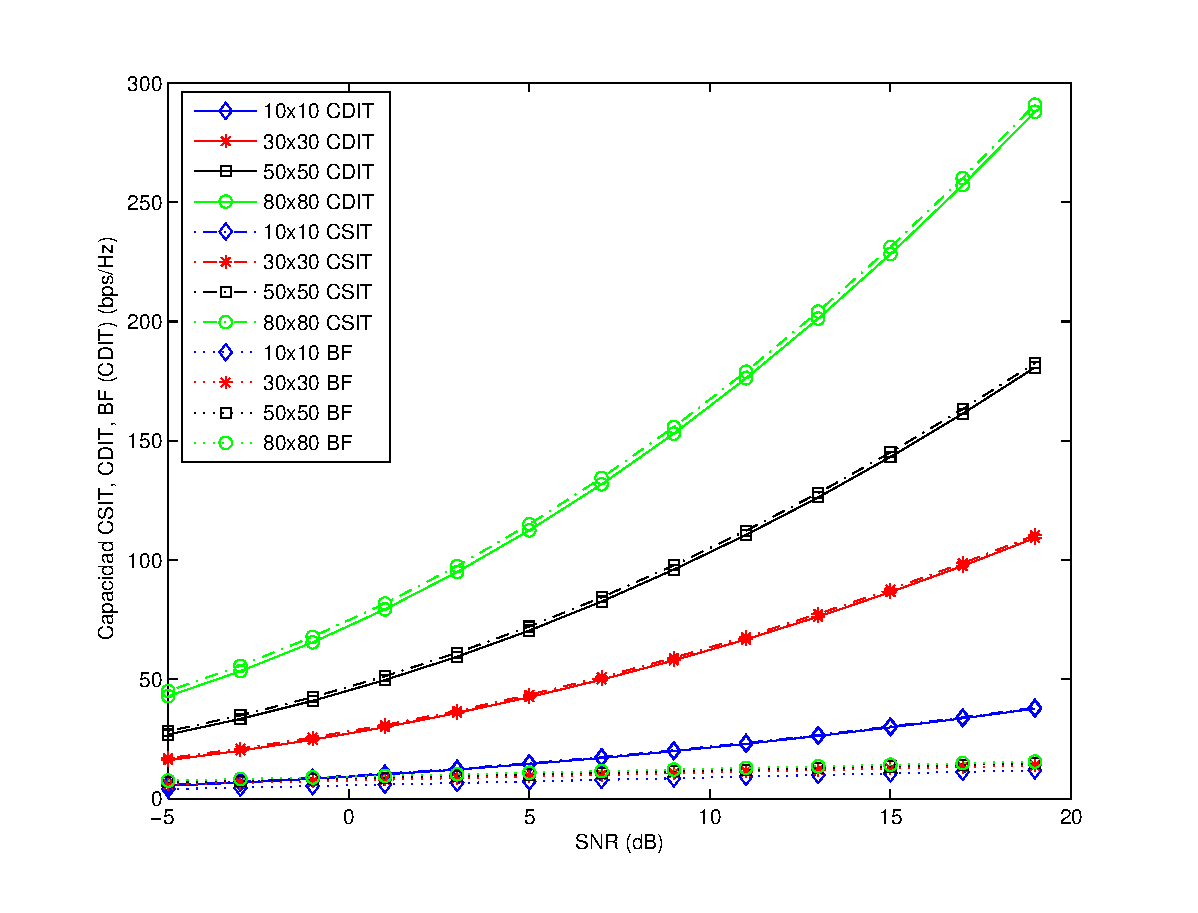
\includegraphics{figuras/CSIT_CDIT_ASD10_dt05.eps}}}}
	\mbox{ \subfigure[$ASD = 20^\circ$]{\resizebox{!}{10cm}		{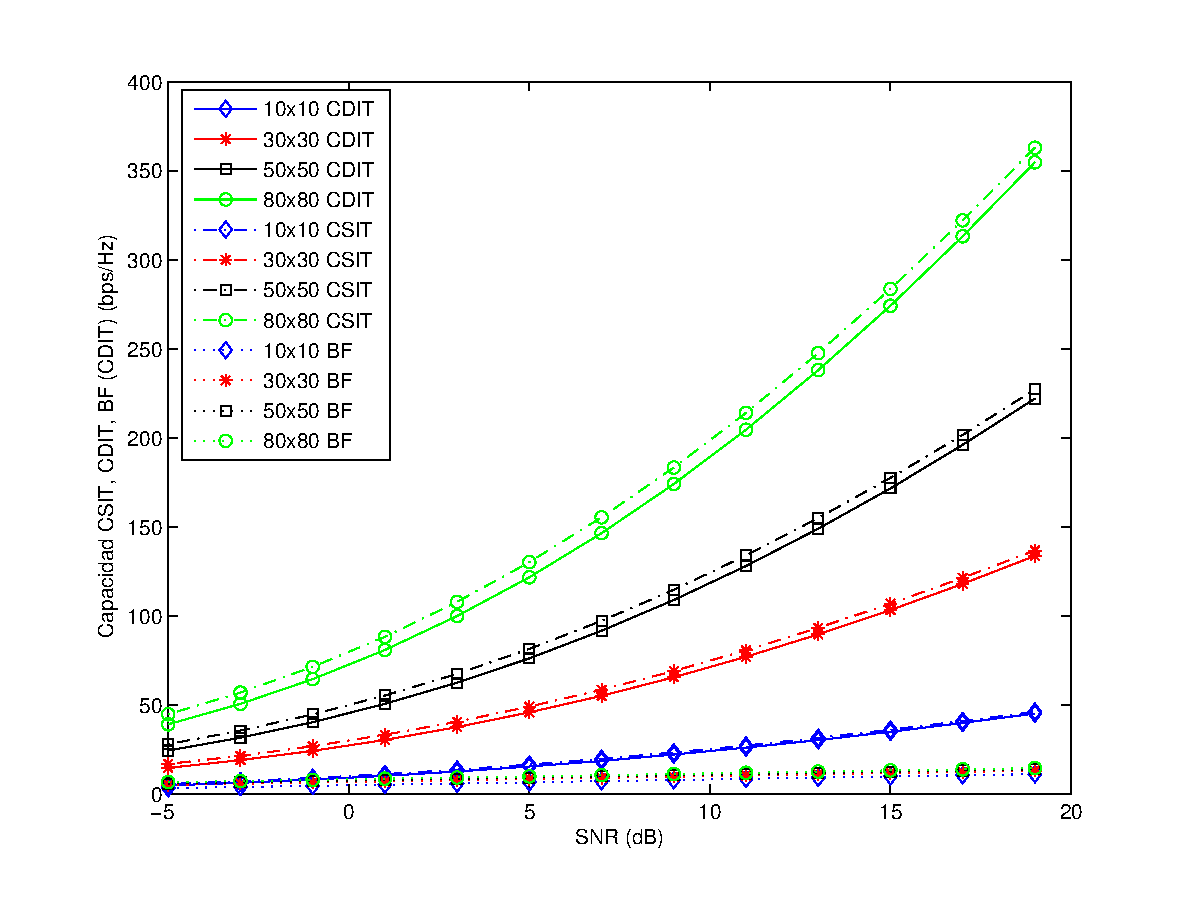
\includegraphics{figuras/CSIT_CDIT_ASD20_dt05.eps}}}}
	\caption{Comparaci�n de la capacidad en escenarios CSIT o CDIT (y diferenciando las dos estrategias de transmisi�n para este �ltimo) para un sistema MIMO Masivo con igual n�mero de antenas transmisoras y receptoras y en el que $d_t = \frac{\lambda}{2}$}
	\label{fig:MN_C_dt05}
\end{figure}

\begin{figure}
\centering
	\mbox{ \subfigure[$ASD = 10^\circ$]{\resizebox{!}{10cm}		{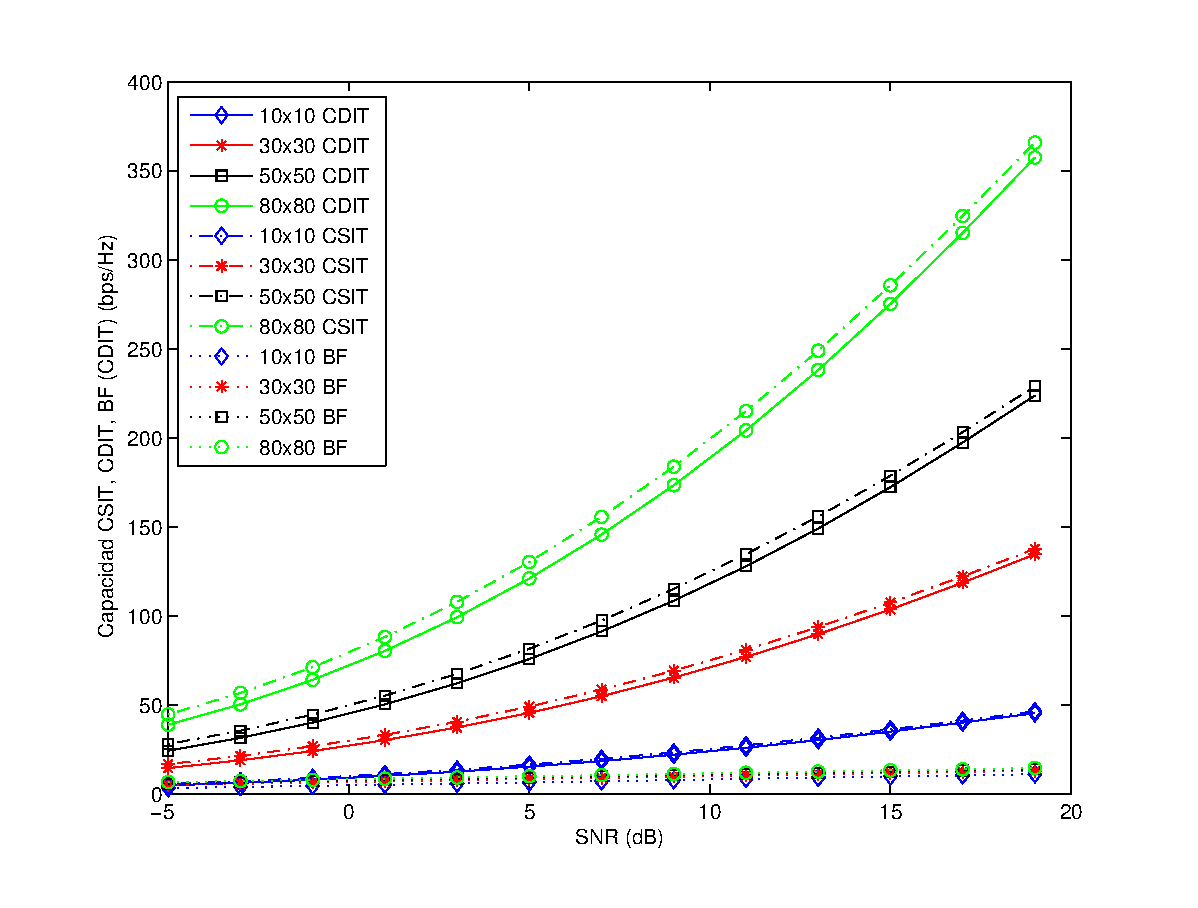
\includegraphics{figuras/CSIT_CDIT_ASD10_dt1.eps}}}}
	\mbox{ \subfigure[$ASD = 20^\circ$]{\resizebox{!}{10cm}		{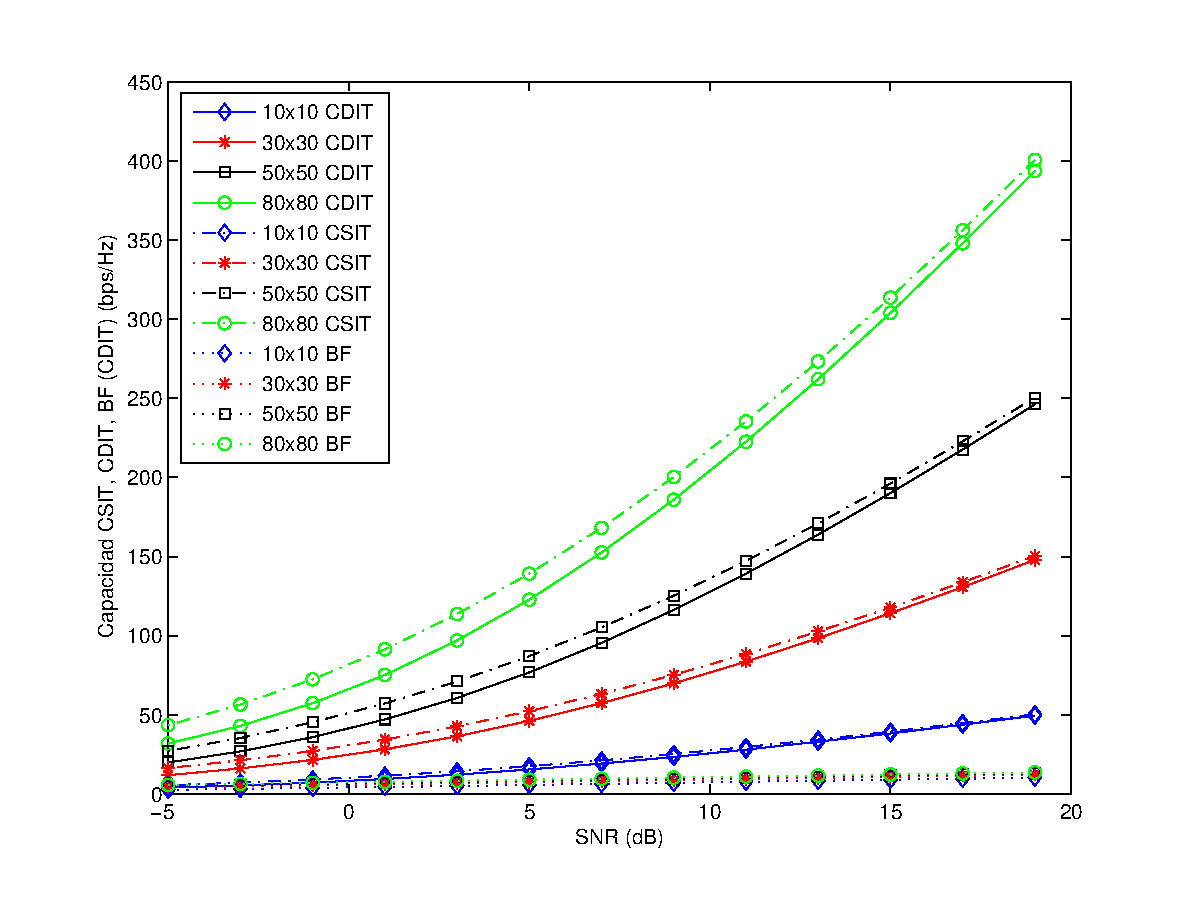
\includegraphics{figuras/CSIT_CDIT_ASD20_dt1.eps}}}}
	\caption{Comparaci�n de la capacidad en escenarios CSIT o CDIT (y diferenciando las dos estrategias de transmisi�n para este �ltimo) para un sistema MIMO Masivo con igual n�mero de antenas transmisoras y receptoras y en el que $d_t = \lambda$}
	\label{fig:MN_C_dt1}
\end{figure}

En primer lugar en la figura (\ref{fig:MN_C_dt05}) nos encontramos en un escenario t�pico en el que la distancia entre antenas transmisoras es igual a $\frac{\lambda}{2}$ mientras que en (\ref{fig:MN_C_dt1}) forzamos un escenario en el que no exista apenas correlaci�n, aumentando la separaci�n entre antenas hasta $\lambda$. En ambos casos, se ve c�mo la estrategia de beamforming generalizado en el escenario CDIT nunca es �ptima frente al resto y, en cuanto a la empleada en CSIT y CDIT, el Water-Filling utilizado en el primer caso supera siempre al algoritmo empleado en el escenario CDIT. Adem�s, esta diferencia es mayor cuanto menor es el nivel de $\snr$ y va disminuyendo conforme aumenta este par�metro. 

Para ilustrar de forma m�s clara los resultados obtenidos, lo haremos a trav�s de la tabla \ref{tabla_mn} en la que se comparan los valores obtenidos de capacidad para un escenario de $ASD = 10^\circ$ y $d_t = \frac{\lambda}{2}$ y para diferentes valores tanto de $\snr$ como del n�mero de antenas. De nuevo, con respecto a este �ltimo par�metro, nos interesa conocer el comportamiento en los extremos; es decir, en escenarios con pocas antenas o muchas antenas, especialmente este �ltimo.  

\begin{sidewaystable}[htbp]
\begin{center}
\begin{tabular}{cc|c|c|c|c|c|c|c|c|c|}
\cline{3-11}
                                                &    & \multicolumn{3}{c|}{10 antenas} & \multicolumn{3}{c|}{60 antenas} & \multicolumn{3}{c|}{80 antenas} \\ \cline{3-11} 
                                                &    & CSIT    & CDIT    & Diferencia  & CSIT    & CDIT    & Diferencia  & CSIT    & CDIT    & Diferencia  \\ \hline
\multicolumn{1}{|c|}{\multirow{6}{*}{SNR (dB)}} & -5 & 5,760   & 5,404   & 0,302       & 33,87   & 32,23   & 1,64        & 45,12   & 42,96   & 2,16        \\ \cline{2-11} 
\multicolumn{1}{|c|}{}                          & 1  & 10,51   & 10,16   & 0,35        & 61,45   & 59,59   & 1,86        & 81,8    & 79,34   & 2,46        \\ \cline{2-11} 
\multicolumn{1}{|c|}{}                          & 5  & 14,89   & 14,51   & 0,38        & 86,45   & 84,48   & 1,97        & 115     & 112,4   & 2,6         \\ \cline{2-11} 
\multicolumn{1}{|c|}{}                          & 9  & 20,28   & 19,88   & 0,4         & 117,1   & 115     & 2,1         & 155,8   & 153     & 2,8         \\ \cline{2-11} 
\multicolumn{1}{|c|}{}                          & 15 & 30,27   & 29,84   & 0,43        & 173,8   & 171,6   & 2,2         & 231,2   & 228,2   & 3           \\ \cline{2-11} 
\multicolumn{1}{|c|}{}                          & 19 & 38,16   & 37,73   & 0,43        & 218,7   & 216,5   & 2,2         & 290,9   & 287,9   & 8,55        \\ \hline
\end{tabular}
\caption{Capacidad (bps/Hz) para un sistema MIMO masivo con el mismo n�mero de antenas en transmisi�n que en recepci�n. Comparaci�n entre los escenarios CSIT y CDIT para 10, 60 y 80 antenas.}
\label{tabla_mn}
\end{center}
\end{sidewaystable}

Mostraremos en estas tablas los resultados para el escenario CSIT y el CDIT, pues como comprobaremos en la secci�n \ref{sec:comp} el algoritmo de beamforming nunca superar� al propuesto en la secci�n \ref{sec:cdit} por lo que no tendremos en cuenta dicha estrategia en esta comparaci�n. 

Como se ve en la tabla \ref{tabla_mn}, en estas condiciones la diferencia entre los dos algoritmos es muy peque�a. Evidentemente, los resultados obtenidos en CSIT son mejores que los obtenidos en CDIT, pues al tener conocimiento del canal y no �nicamente de sus estad�sticos, las condiciones son mejores. El algoritmo Water-Filling empleado en el escenario CSIT proporciona entre 0.3 y 0.4 bps/Hz m�s que el algoritmo implementado para el escenario CDIT y la diferencia entre estos dos casos aumenta muy poco a medida que los valores de la $\snr$ aumentan. 

Sin embargo, al observar los datos correspondientes a 60 y 80 antenas podemos ver que con un n�mero elevado de antenas en transmisi�n y en recepci�n la diferencia entre los dos escenarios se hace notable. Con 60 antenas la diferencia entre los dos casos es de alrededor de 2 bps/Hz y la variaci�n con respecto a la $\snr$ es mayor que la que ten�amos para 10 antenas. Por �ltimo, para 80 antenas es cuando la diferencia entre los dos escenarios se hace mayor partiendo desde 2.16 bps/Hz para una $\snr$ de -5 dB y llegando hasta 3 bps/Hz para 19 dB. Estos 3 bits extra que estamos consiguiendo en el caso CSIT son 3 bits m�s que podemos incluir en la constelaci�n y aumentar de esta forma el n�mero de s�mbolos posibles a transmitir.

\subsubsection{Sistema MIMO Masivo con $M$ antenas transmisoras y $4$ antenas receptoras}

\begin{figure}
\centering
	\mbox{ \subfigure[$ASD = 10^\circ$]{\resizebox{!}{10cm}		{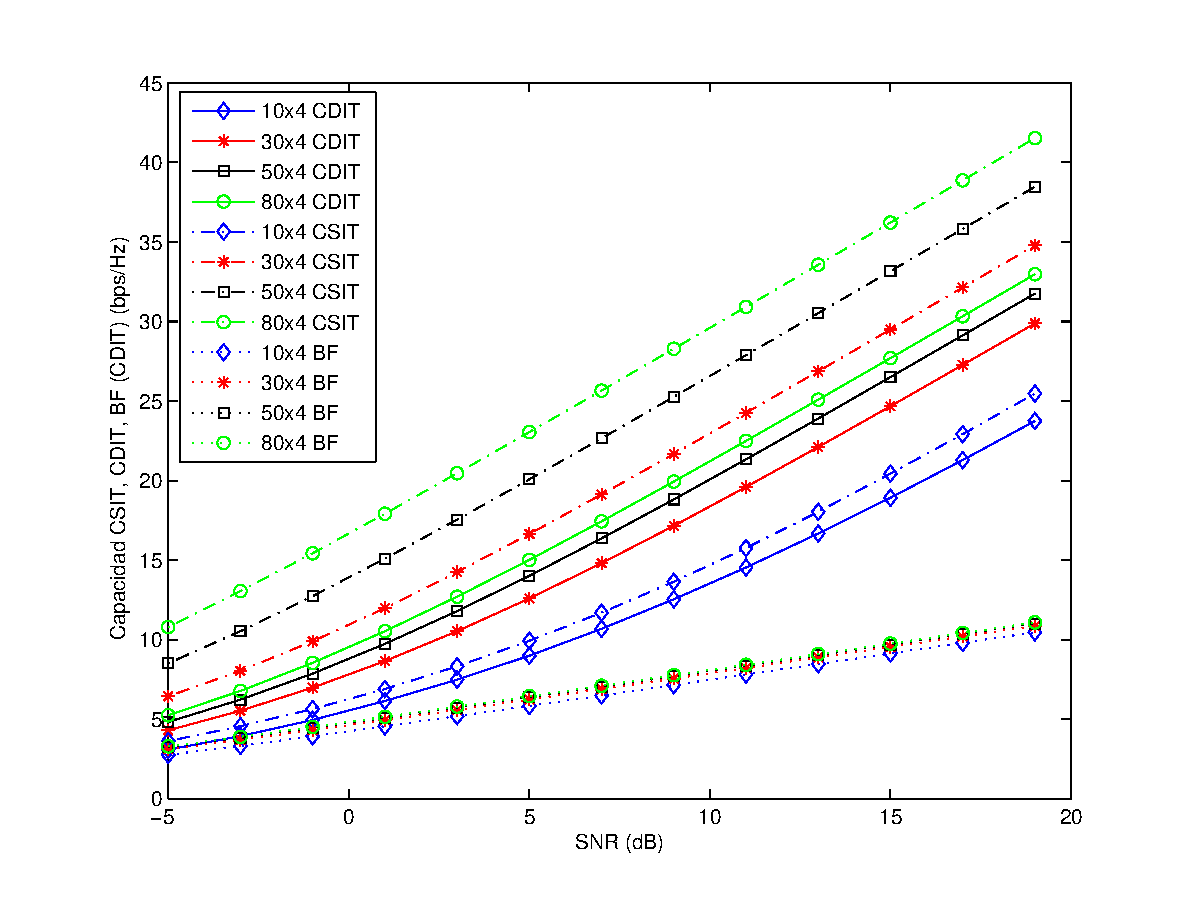
\includegraphics{figuras/CSIT_CDIT_ASD10_dt05_N4.eps}}}}
	\mbox{ \subfigure[$ASD = 20^\circ$]{\resizebox{!}{10cm}		{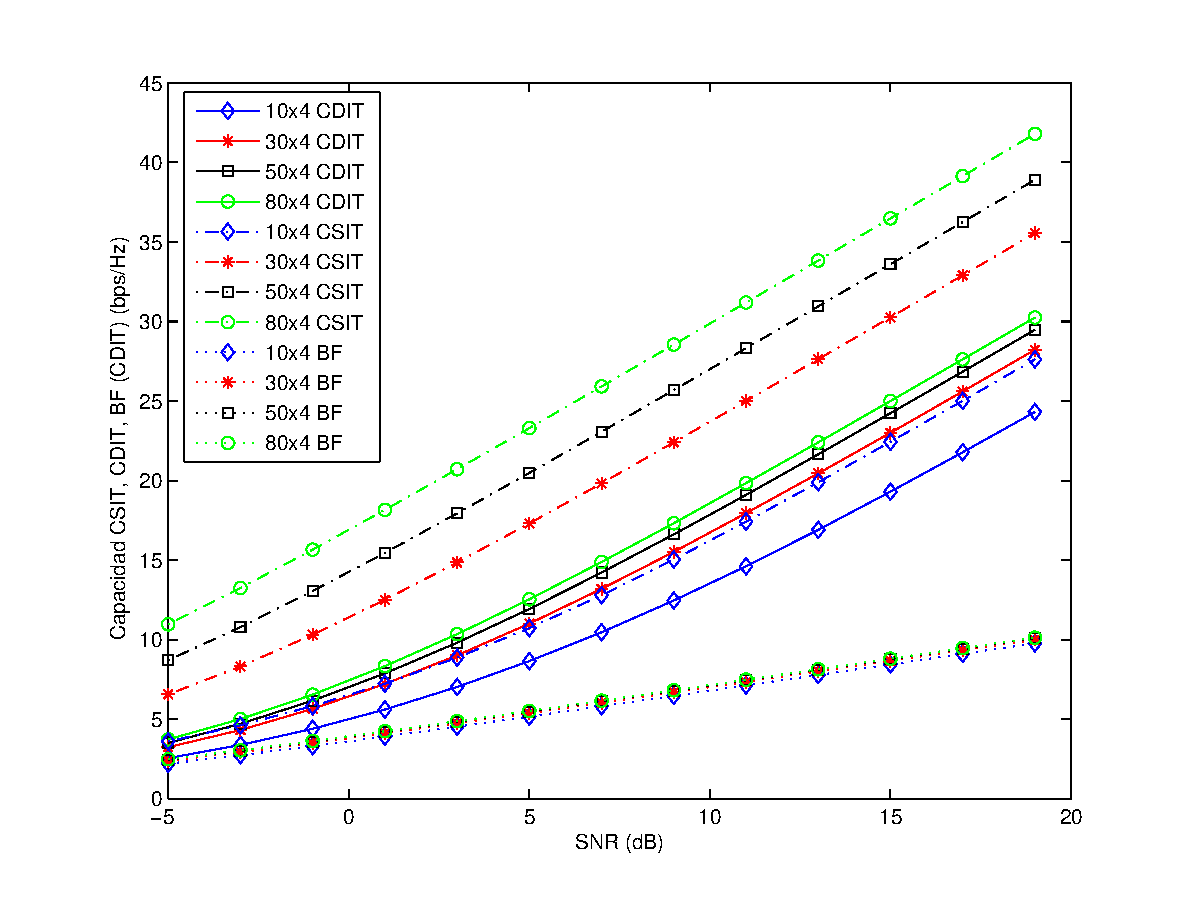
\includegraphics{figuras/CSIT_CDIT_ASD20_dt05_N4.eps}}}}
	\caption{Comparaci�n de la capacidad en escenarios CSIT o CDIT (y diferenciando las dos estrategias de transmisi�n para este �ltimo) para un sistema MIMO Masivo con $M$ antenas transmisoras y $4$ receptoras y en el que $d_t = \frac{\lambda}{2}$}
	\label{fig:MN4_C_dt05}
\end{figure}

\begin{figure}
\centering
	\mbox{ \subfigure[$ASD = 10^\circ$]{\resizebox{!}{10cm}		{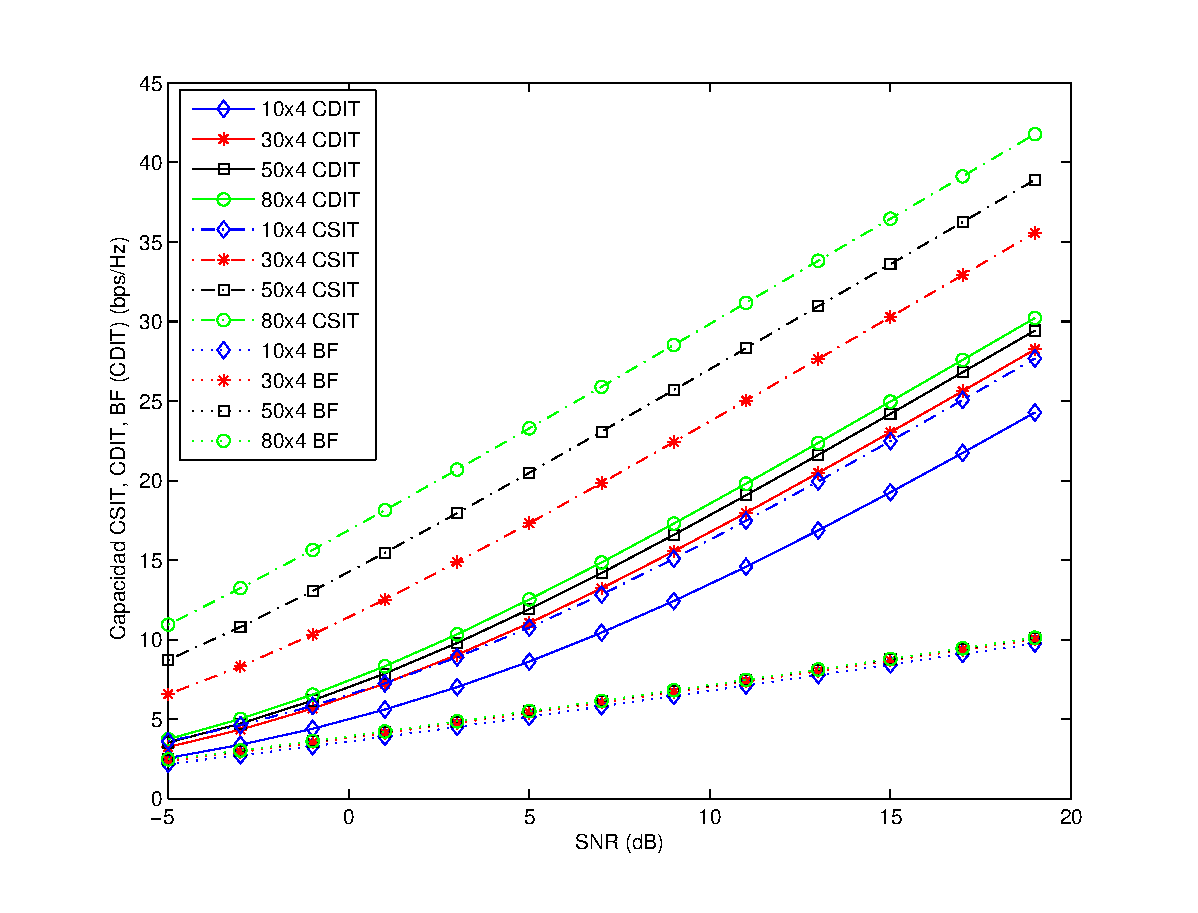
\includegraphics{figuras/CSIT_CDIT_ASD10_dt1_N4.eps}}}}
	\mbox{ \subfigure[$ASD = 20^\circ$]{\resizebox{!}{10cm}		{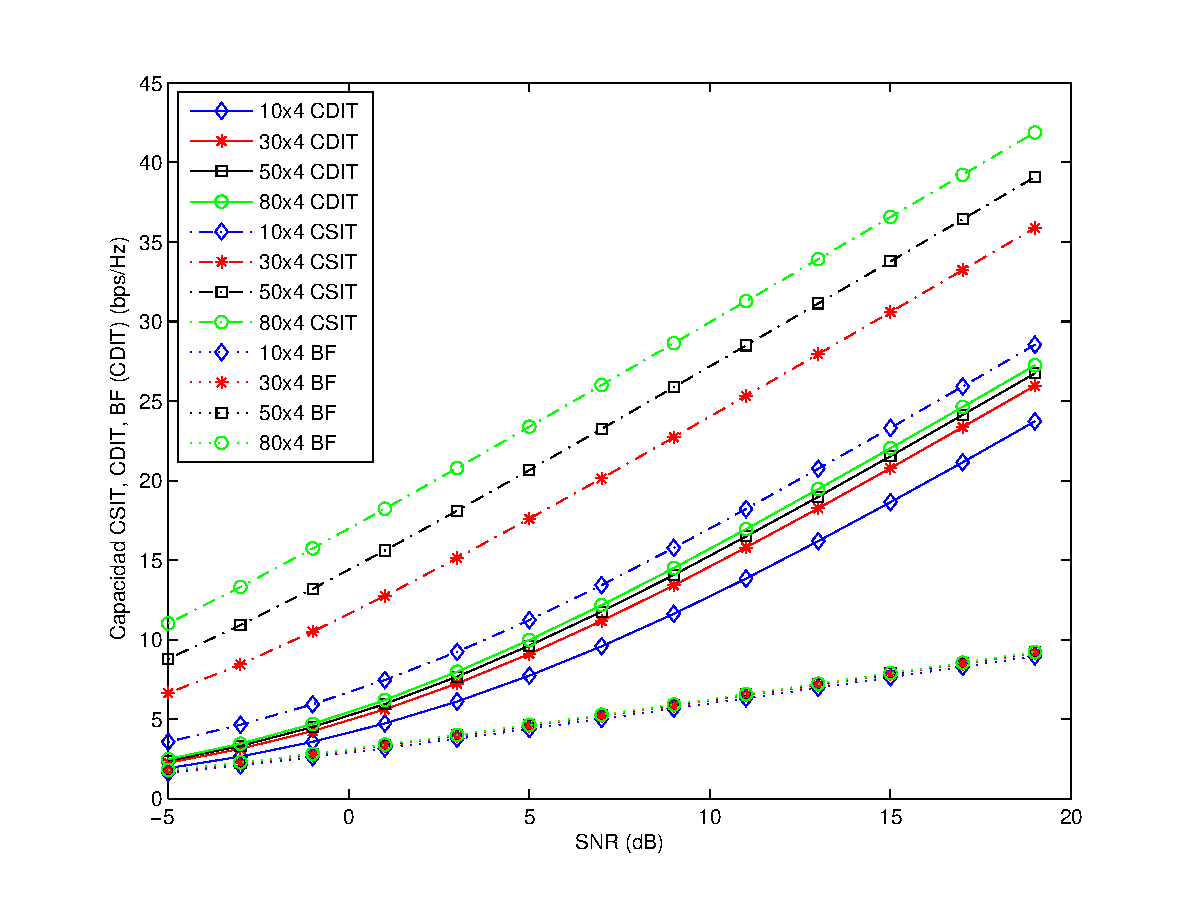
\includegraphics{figuras/CSIT_CDIT_ASD20_dt1_N4.eps}}}}
	\caption{Comparaci�n de la capacidad en escenarios CSIT o CDIT (y diferenciando las dos estrategias de transmisi�n para este �ltimo) para un sistema MIMO Masivo con $M$ antenas transmisoras y $4$ receptoras y en el que $d_t = \lambda$}
	\label{fig:MN4_C_dt1}
\end{figure}

En las figuras (\ref{fig:MN4_C_dt05}) y (\ref{fig:MN4_C_dt1}) se puede ver la evoluci�n de la capacidad con respecto a la $\snr$ para diferentes valores de $ASD$ y $d_t$. En cada gr�fica se muestra adem�s dicha capacidad para diferente n�mero de antenas.

De igual forma que hac�amos en la secci�n anterior, observaremos de forma m�s clara los resultados obtenidos en una tabla en la que podamos comparar el comportamiento en los dos escenarios con respecto a la $\snr$ y al n�mero de antenas transmisoras. 

\begin{sidewaystable}[htbp]
\begin{center}
\begin{tabular}{cc|c|c|c|c|c|c|c|c|c|}
\cline{3-11}
                                                &    & \multicolumn{3}{c|}{10 antenas} & \multicolumn{3}{c|}{60 antenas} & \multicolumn{3}{c|}{80 antenas} \\ \cline{3-11} 
                                                &    & CSIT    & CDIT    & Diferencia  & CSIT    & CDIT    & Diferencia  & CSIT    & CDIT    & Diferencia  \\ \hline
\multicolumn{1}{|c|}{\multirow{6}{*}{SNR (dB)}} & -5 & 4       & 3,082   & 0,541       & 9,3     & 4,981   & 4,319       & 10,79   & 5,246   & 5,544       \\ \cline{2-11} 
\multicolumn{1}{|c|}{}                          & 1  & 6,893   & 6,137   & 0,756       & 16,1    & 10,02   & 6,08        & 17,91   & 10,53   & 7,38        \\ \cline{2-11} 
\multicolumn{1}{|c|}{}                          & 5  & 9,926   & 8,991   & 0,935       & 21,15   & 14,37   & 6,78        & 23,04   & 15,01   & 8,03        \\ \cline{2-11} 
\multicolumn{1}{|c|}{}                          & 9  & 13,64   & 12,53   & 1,11        & 26,35   & 19,22   & 7,13        & 28,28   & 19,94   & 8,34        \\ \cline{2-11} 
\multicolumn{1}{|c|}{}                          & 15 & 20,43   & 18,93   & 1,5         & 34,27   & 26,94   & 7,33        & 36,22   & 27,7    & 8,52        \\ \cline{2-11} 
\multicolumn{1}{|c|}{}                          & 19 & 25,46   & 23,74   & 1,72        & 39,57   & 32,2    & 7,37        & 41,52   & 32,97   & 8,55        \\ \hline
\end{tabular}
\caption{Capacidad (bps/Hz) para un sistema MIMO masivo con $4$ antenas en recepci�n y 10, 60 y 80 antenas en transmisi�n. Comparaci�n entre los escenarios CSIT y CDIT}
\label{tabla_masivo}
\end{center}
\end{sidewaystable}

En primer lugar, en la tabla \ref{tabla_masivo} encontramos los resultados para un escenario con 10, 60 y 80 antenas en transmisi�n y 4 en recepci�n. Para 10 antenas, la diferencia entre las dos estrategias oscila en torno a 1 bps/Hz, una diferencia mayor a la que obten�amos para el caso de 10 antenas transmisoras y receptoras. Podemos ver como esta diferencia se hace mucho mayor cuando aumentamos el n�mero de antenas transmisoras. Para el caso de 60 la diferencia va desde 4.319 bps/Hz hasta 7.37 bps/Hz y para 80 antenas, esta diferencia var�a desde 5.544 bps/Hz para una $\snr$ de -5 dB hasta 8.55 bps/Hz para una $\snr$ de 19 dB.

\subsection{Alta $\snr$}

Antes de presentar los resultados obtenidos a trav�s de la simulaciones realizadas, cabe destacar que existen aproximaciones anal�ticas para calcular la capacidad y la eficiencia espectral de un sistema de comunicaciones tanto para altas $\snr$ como para bajas. Para ello, a menudo es conveniente expresar la capacidad no s�lo como una funci�n de la relaci�n se�al a ruido sino tambi�n de la energ�a por bit transmitida relativa al nivel de ruido $\left(\frac{E_b}{N_0}\right)$

\begin{equation}
\frac{E_b}{N_0} = \frac{E[||\mix||^2]}{N_0C(\snr)} = \frac{\snr}{gC(\snr)}
\end{equation}

De \cite{Tulino05}, para valores elevados de $\snr$ la capacidad se comporta de la siguiente forma:

\begin{equation}
C(\snr) = S_{\infty} \left(\frac{\snr}{3 \text{dB}} - L_{\infty} \right) + o(1)
\end{equation}

donde $S_{\infty}$ denota la pendiente a alta $\snr$ en bps/Hz/(3 dB) 
y $L_{\infty}$ 
representa el offset de potencia respecto a un canal de referencia ortogonal tal que $\frac{1}{M}\miH \miH ^H = \mathbf{I}$. Relacionando la capacidad con $\frac{E_b}{N_0}$ obtenemos

\begin{equation}
\frac{E_b}{N_0}|_{dB} = \left(\frac{C}{S_{\infty}} + L_{\infty} \right)\text{3 dB} - 10\text{log}_{10}C - g|_{\text{dB}} + o(1)
\end{equation}

Como se ve, $S_{\infty}$ representa tanto la pendiente en t�rminos de $\snr$ como en t�rminos $\frac{E_b}{N_0}$. 

Hemos hecho uso de esta aproximaci�n para comprobar si los resultados obtenidos en las simulaciones son coherentes. 

\subsubsection{Sistema MIMO con el mismo n�mero de antenas transmisoras y receptoras}

Para un valor de $\snr$ de 19 dB se muestran los resultados de capacidad, compar�ndola en funci�n de los diferentes escenarios expuestos. En primer lugar en la figura (\ref{fig:MN_COMP_HS_DT}) podemos observar dicha comparaci�n para dos valores concretos del �ngulo de dispersi�n, por lo que podremos examinar su evoluci�n con respecto a la distancia entre las antenas. A medida que esta aumenta, el valor de la capacidad lo hace tambi�n, como es de esperar pues cuando la correlaci�n es menor nos encontramos en mejores condiciones. 

\begin{figure}
\centering
	\mbox{ \subfigure[$ASD = 10^\circ$]{\resizebox{!}{10cm}		{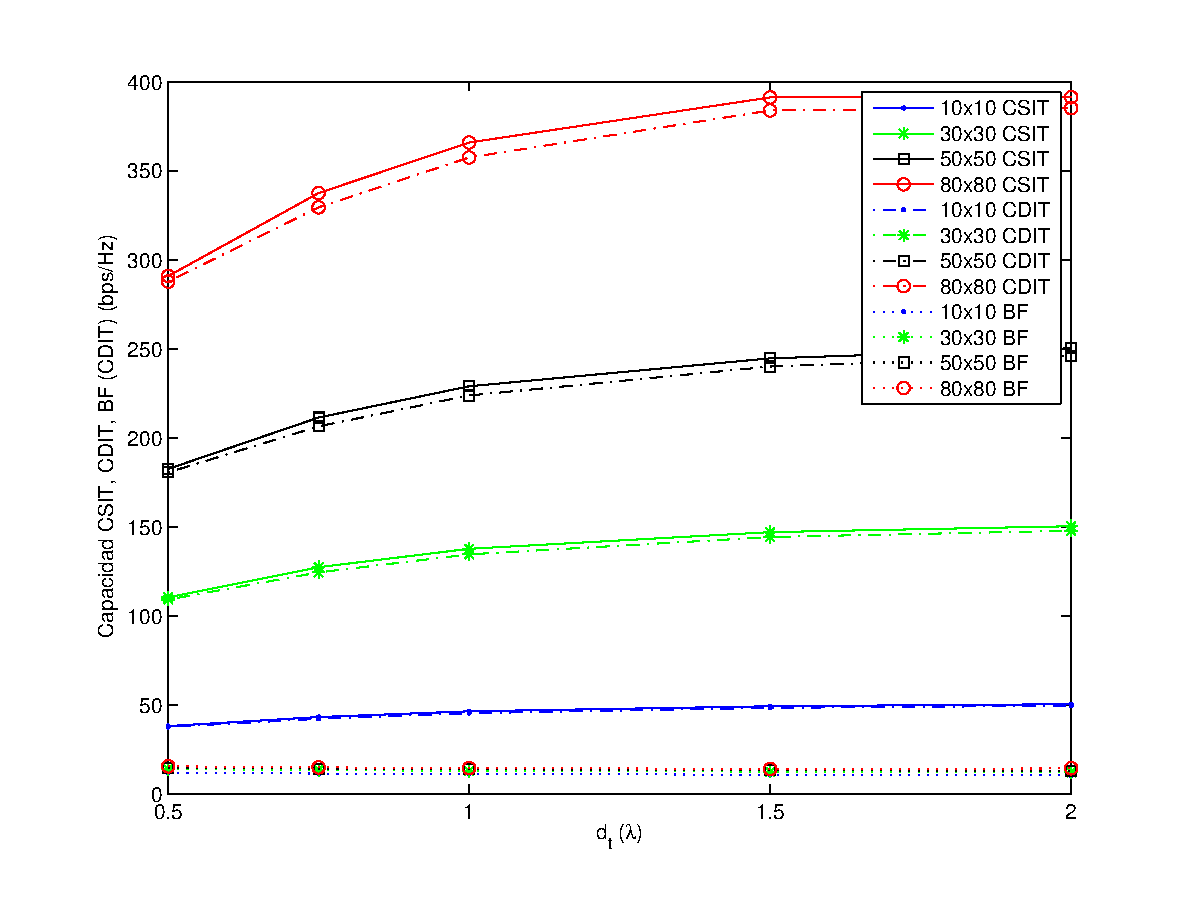
\includegraphics{figuras/CDIT_CSIT_SNR19_ASD10.eps}}}}
	\mbox{ \subfigure[$ASD = 20^\circ$]{\resizebox{!}{10cm}		{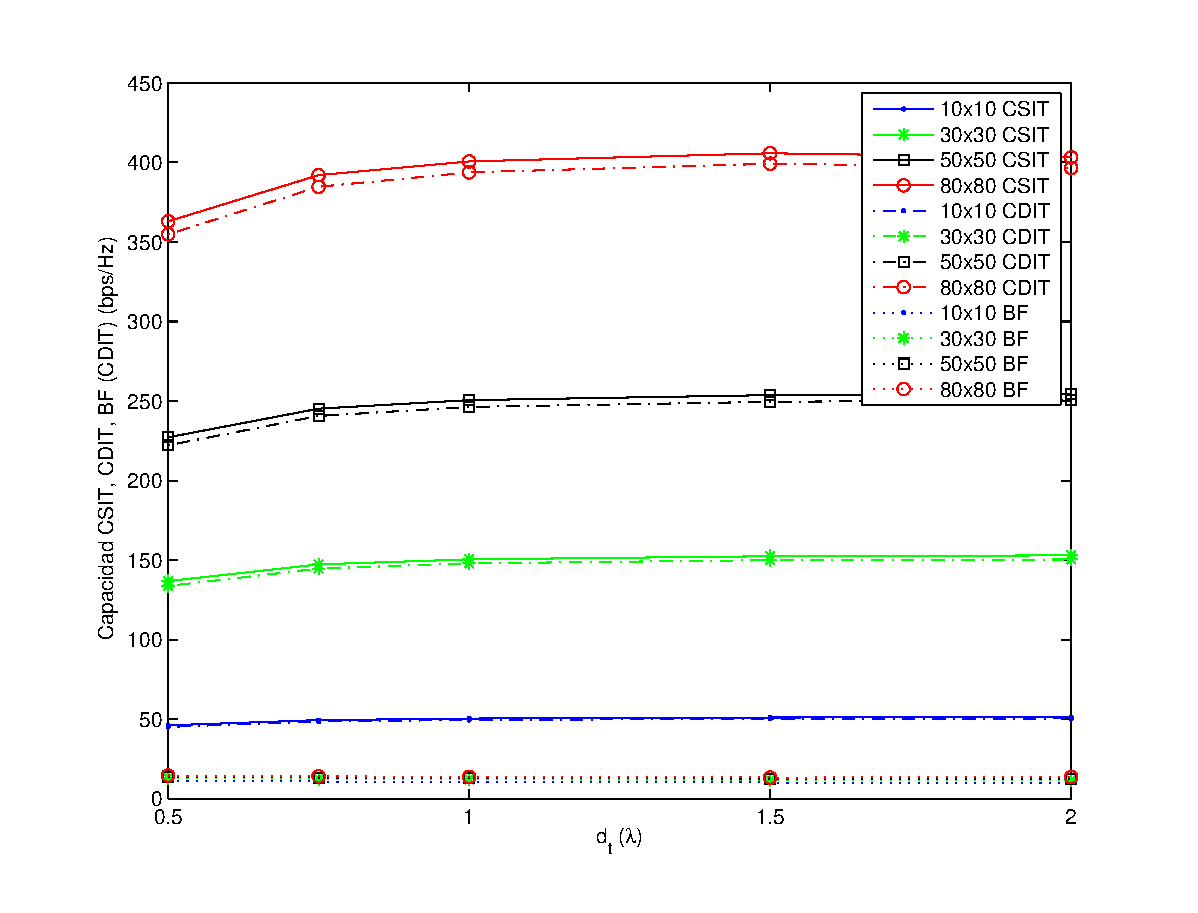
\includegraphics{figuras/CDIT_CSIT_SNR19_ASD20.eps}}}}
	\caption{Comparaci�n de la capacidad en escenarios CSIT o CDIT (y diferenciando las dos estrategias de transmisi�n para este �ltimo) de un sistema MIMO Masivo con igual n�mero de antenas transmisoras y receptoras para $\snr = 19$ dB. Evoluci�n con respecto a la distancia entre antenas transmisoras.}
	\label{fig:MN_COMP_HS_DT}
\end{figure}

En la figura (\ref{fig:MN_COMP_HS_ASD}) lo que podemos ver es la evoluci�n con respecto a $ASD$, es decir, al �ngulo de dispersi�n del transmisor. Estas gr�ficas tienen un comportamiento similar a una funci�n logar�tmica, es decir, crecen r�pidamente cuando nos encontramos en valores del $ASD$ bajos y se estabilizan a medida que este �ngulo se hace mayor. Este comportamiento se acerca cada vez m�s a un comportamiento logar�tmico a medida que nos encontramos en mejores condiciones ($d_t$ aumenta), y el momento en el que empieza a tener un comportamiento constante sucede para valores menores del $ASD$. 


\begin{figure}
\centering
	\mbox{ \subfigure[$d_t = \frac{\lambda}{2}$]{\resizebox{!}{10cm}		{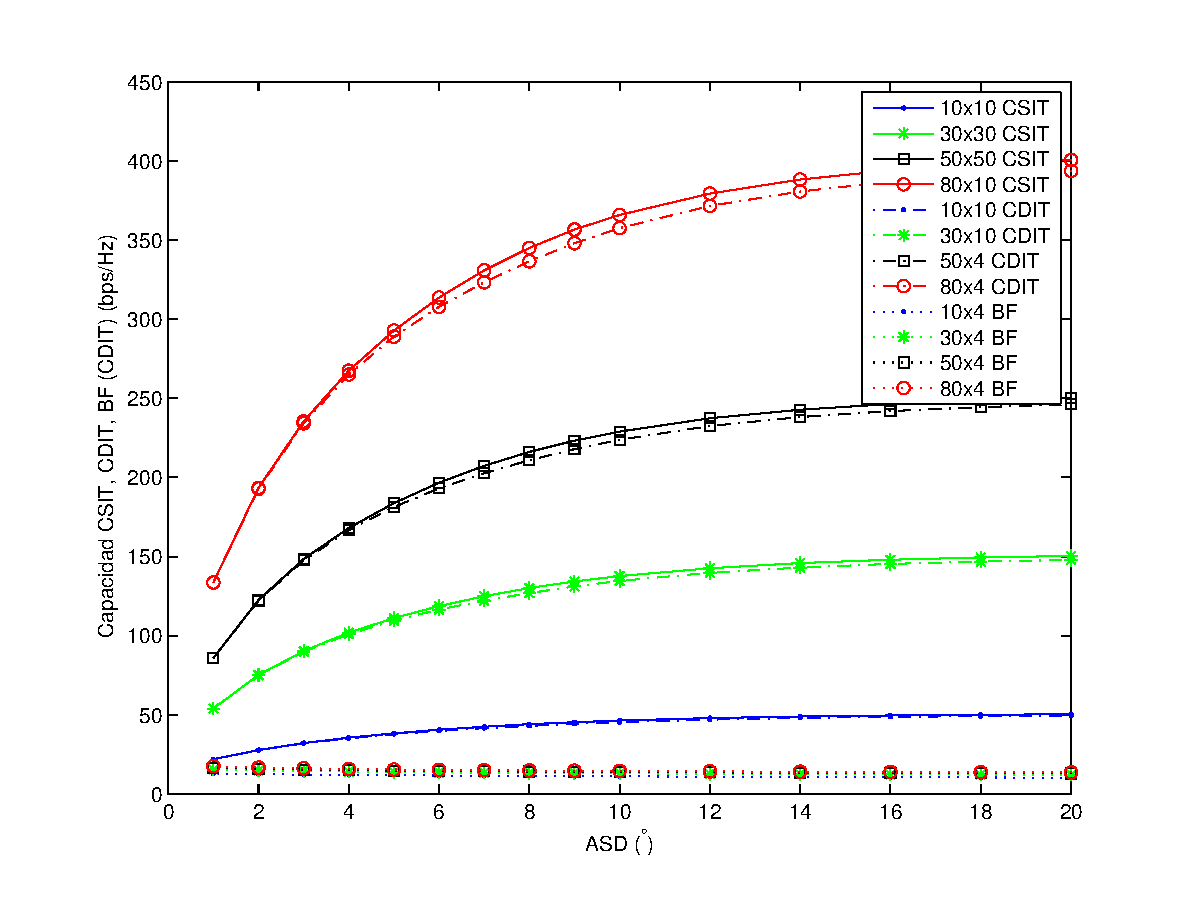
\includegraphics{figuras/CDIT_CSIT_SNR19_dt05.eps}}}}
	\mbox{ \subfigure[$d_t = \lambda$]{\resizebox{!}{10cm}		{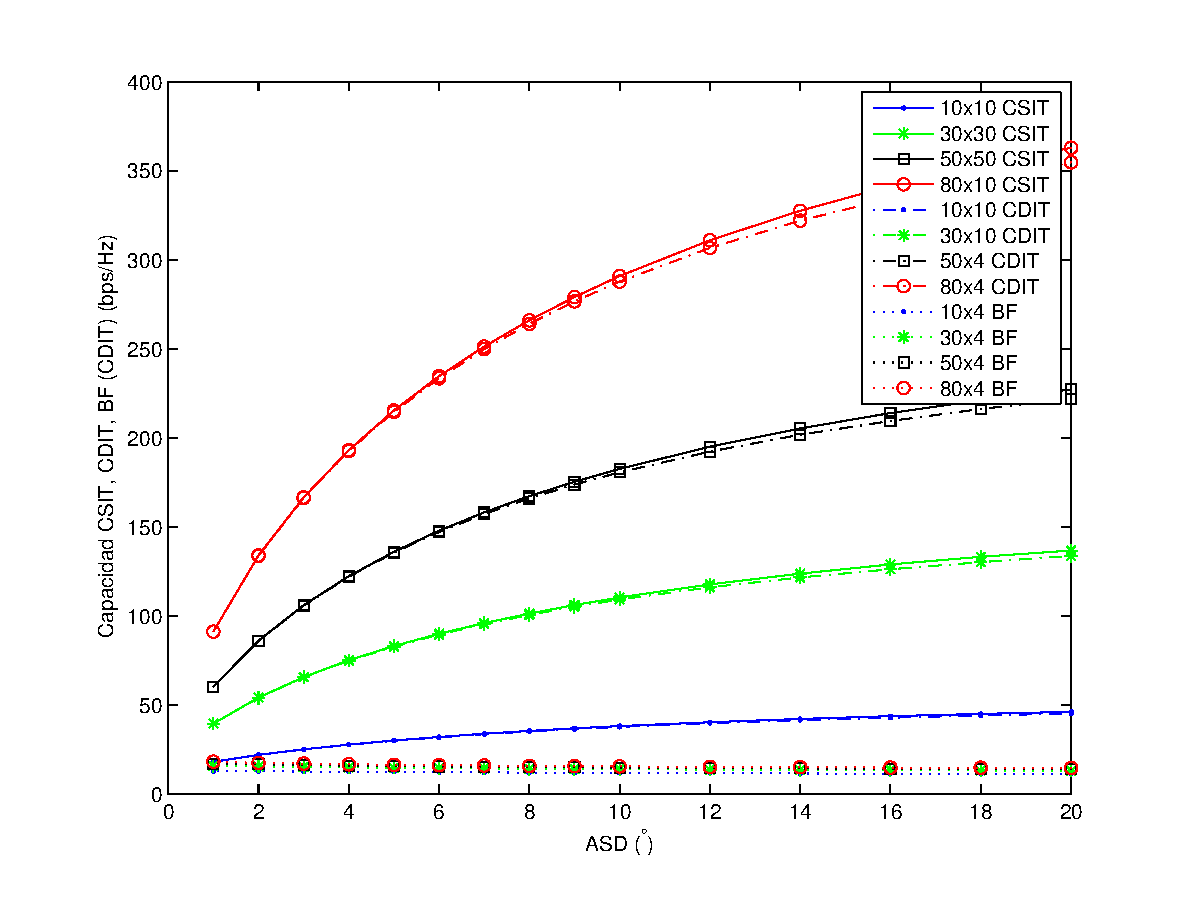
\includegraphics{figuras/CDIT_CSIT_SNR19_dt1.eps}}}}
	\caption{Comparaci�n de la capacidad en escenarios CSIT o CDIT (y diferenciando las dos estrategias de transmisi�n para este �ltimo) de un sistema MIMO Masivo con igual n�mero de antenas transmisoras y receptoras para $\snr = 19$ dB. Evoluci�n con respecto al �ngulo de dispersi�n en el transmisor.}
	\label{fig:MN_COMP_HS_ASD}
\end{figure}

En ambos casos las diferencias existentes entre los dos escenarios son m�nimas, pues para valores elevados de $\snr$ los algoritmos empleados en ambos casos tienen muy buena respuesta. 


\subsubsection{Sistema MIMO masivo con M antenas transmisoras y 4 antenas receptoras}

De nuevo, para un valor de $\snr$ de 19 dB se muestran los resultados de capacidad, compar�ndola en funci�n de los diferentes escenarios expuestos. En primer lugar en la figura (\ref{fig:MN_COMP_HS_DT_N4}) podemos observar dicha comparaci�n para dos valores concretos del �ngulo de dispersi�n, por lo que podremos examinar su evoluci�n con respecto a la distancia entre las antenas; mientras que en la figura (\ref{fig:MN_COMP_HS_ASD_N4}) lo que veremos ser� la evoluci�n con respecto al �ngulo de dispersi�n. 

\begin{figure}
\centering
	\mbox{ \subfigure[$ASD = 10^\circ$]{\resizebox{!}{10cm}		{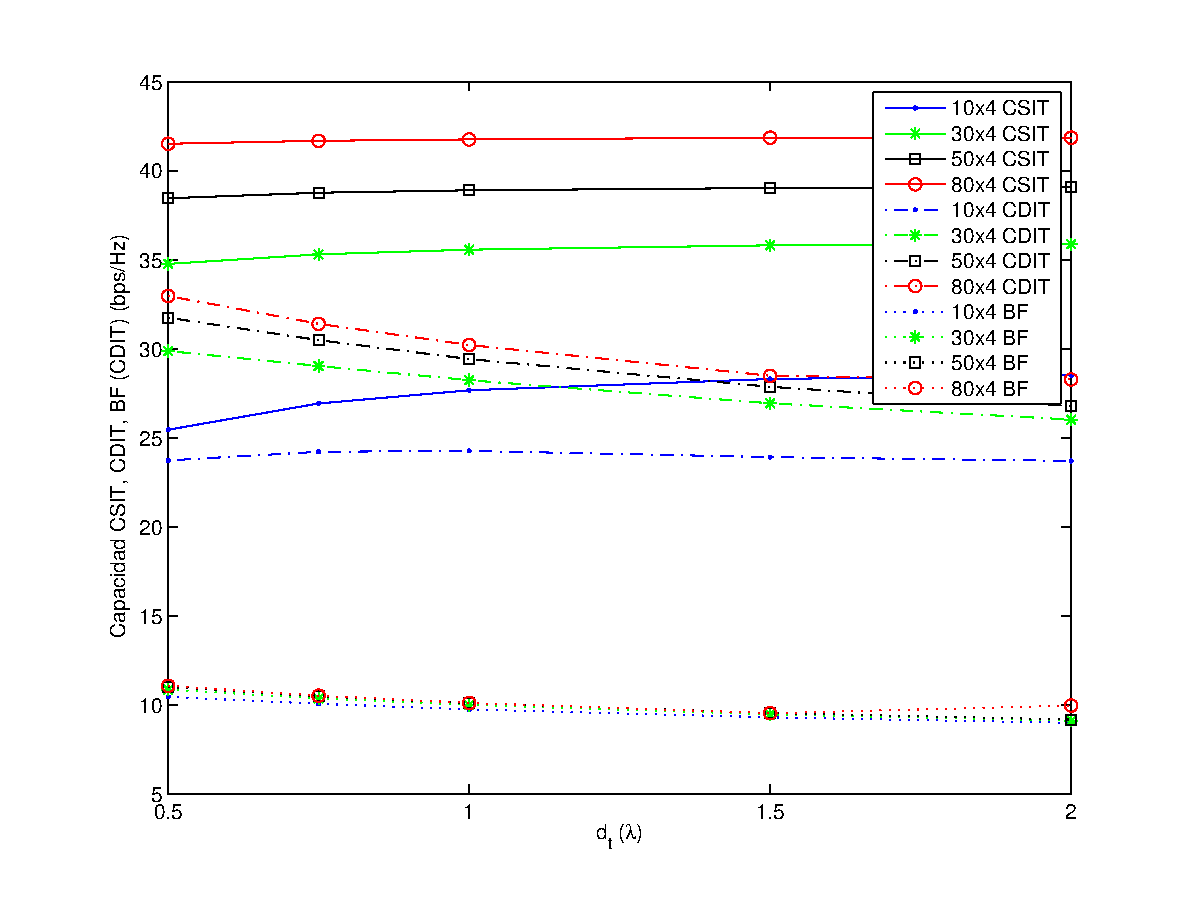
\includegraphics{figuras/CDIT_CSIT_SNR19_ASD10_N4.eps}}}}
	\mbox{ \subfigure[$ASD = 20^\circ$]{\resizebox{!}{10cm}		{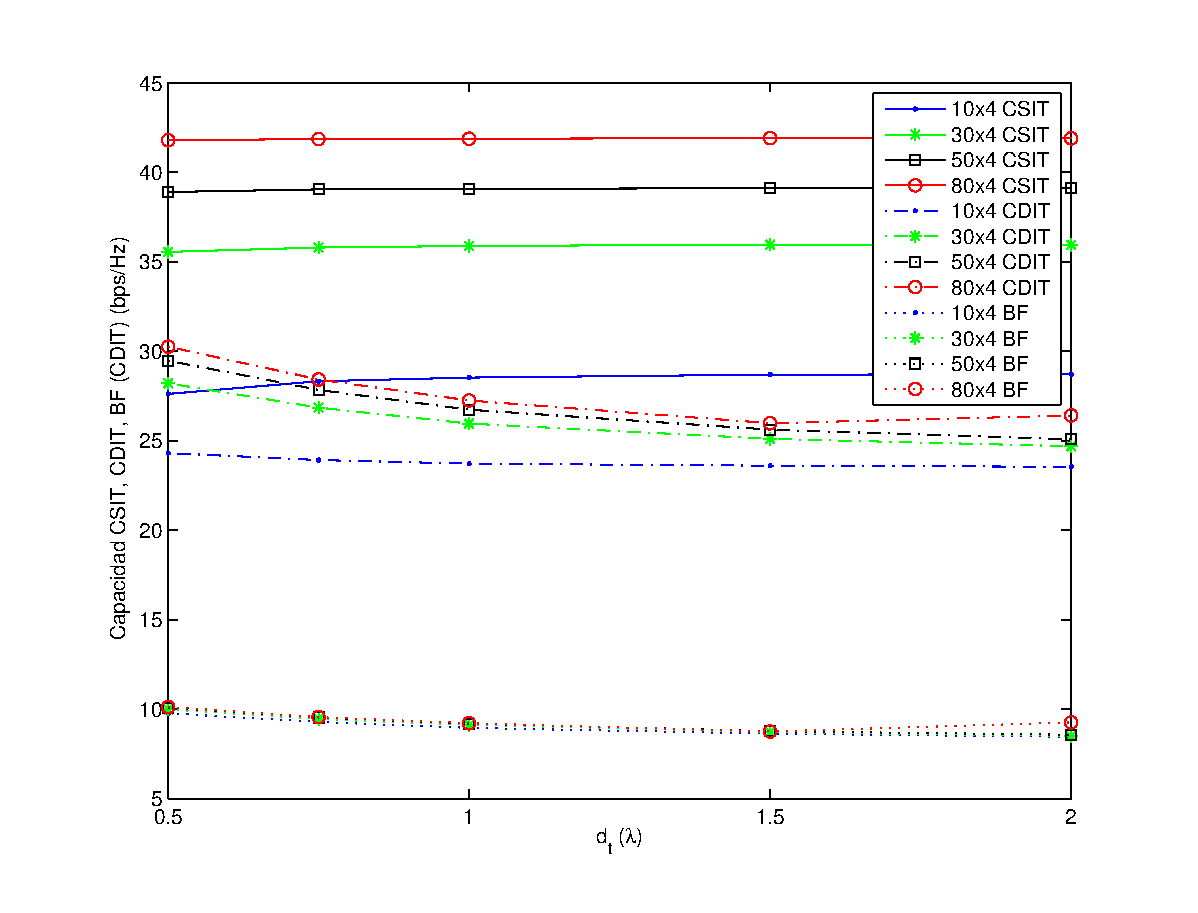
\includegraphics{figuras/CDIT_CSIT_SNR19_ASD20_N4.eps}}}}
	\caption{Comparaci�n de la capacidad en escenarios CSIT o CDIT (y diferenciando las dos estrategias de transmisi�n para este �ltimo) de un sistema MIMO Masivo con $M$ antenas transmisoras y $4$ receptoras para $\snr = 19$ dB. Evoluci�n con respecto a la distancia entre antenas transmisoras.}
	\label{fig:MN_COMP_HS_DT_N4}
\end{figure}


\begin{figure}
\centering
	\mbox{ \subfigure[$d_t = \frac{\lambda}{2}$]{\resizebox{!}{10cm}		{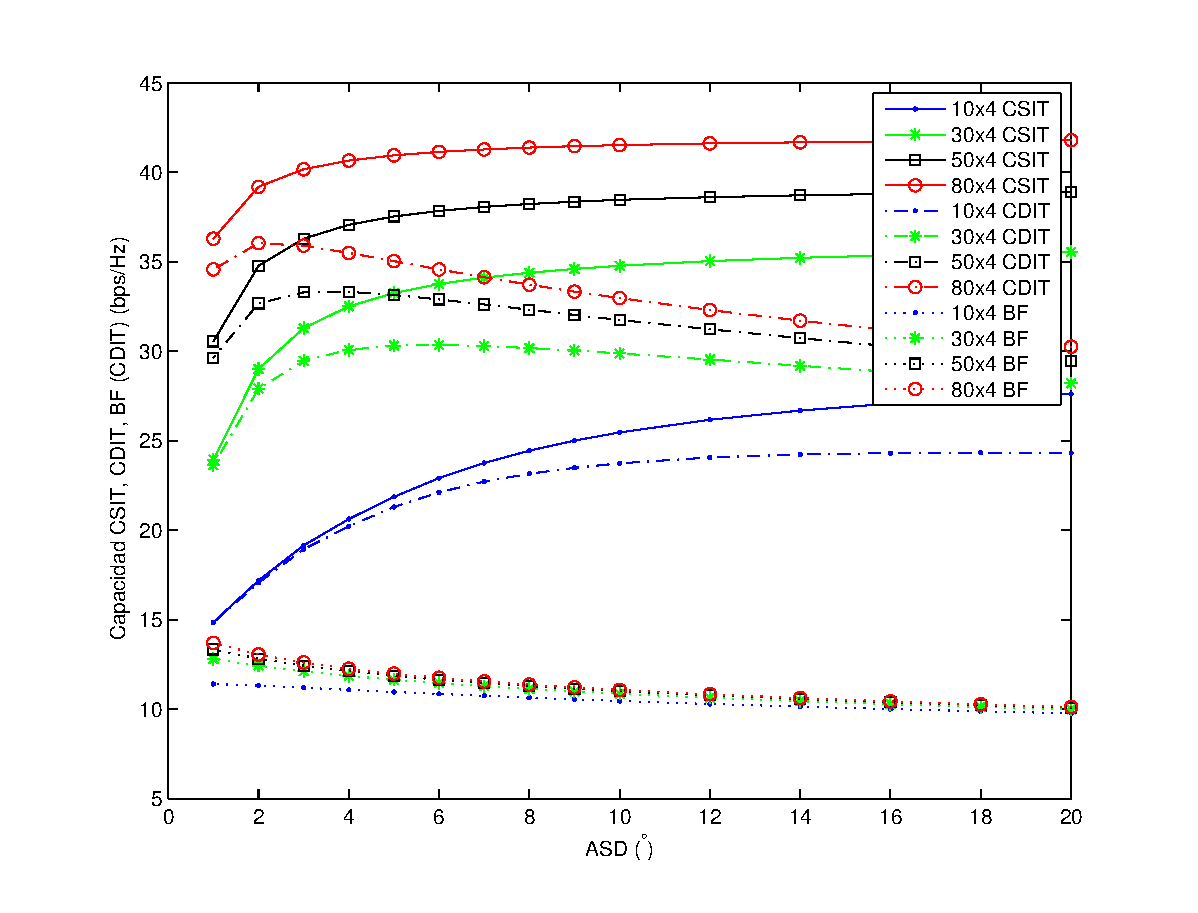
\includegraphics{figuras/CDIT_CSIT_SNR19_dt05_N4.eps}}}}
	\mbox{ \subfigure[$d_t = \lambda$]{\resizebox{!}{10cm}		{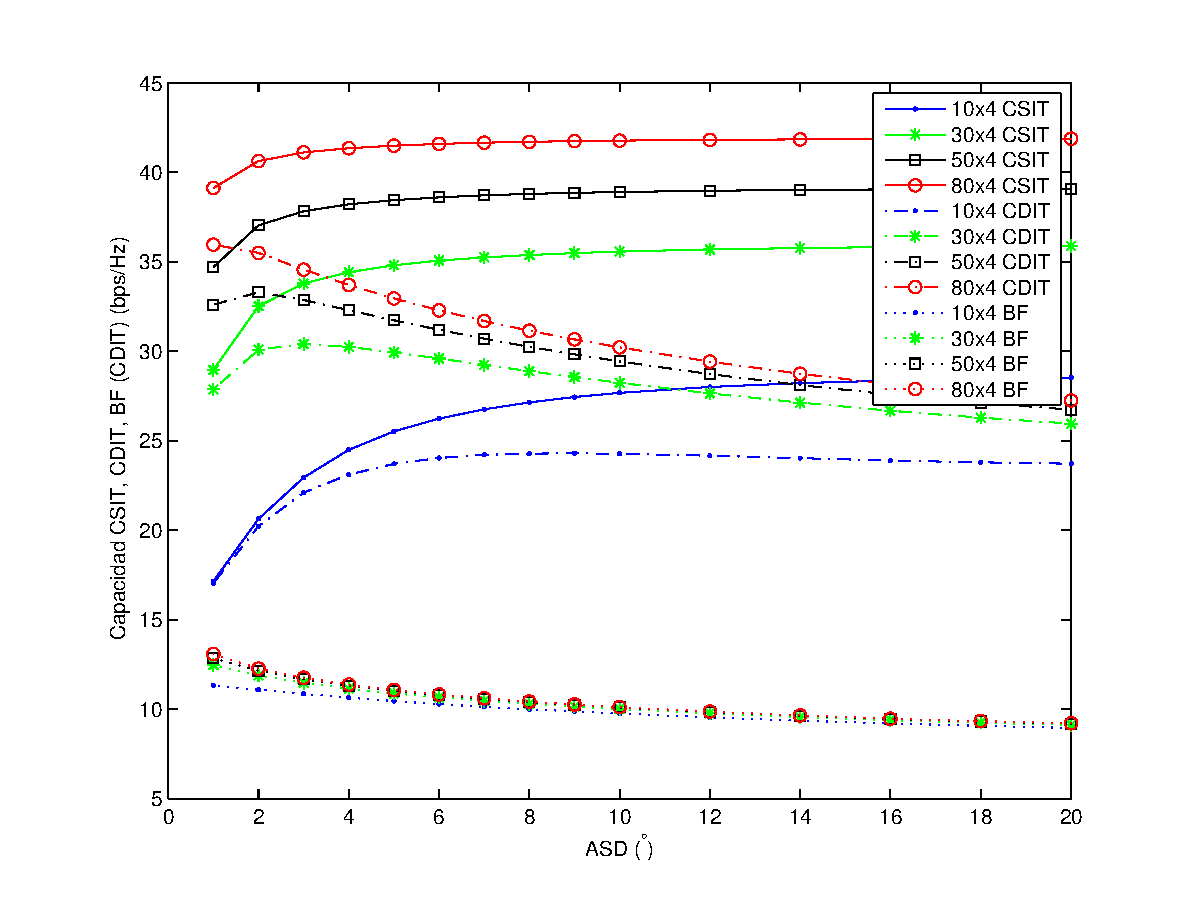
\includegraphics{figuras/CDIT_CSIT_SNR19_dt1_N4.eps}}}}
	\caption{Comparaci�n de la capacidad en escenarios CSIT o CDIT (y diferenciando las dos estrategias de transmisi�n para este �ltimo) de un sistema MIMO Masivo con $M$ antenas transmisoras y $4$ receptoras para $\snr = 19$ dB. Evoluci�n con respecto al �ngulo de dispersi�n en el transmisor.}
	\label{fig:MN_COMP_HS_ASD_N4}
\end{figure}

Mientras que el comportamiento en el escenario CSIT tiende a estabilizarse a partir de un cierto valor de $ASD$ o $d_t$ (valor que ser� menor a medida que las condiciones mejoren bien aumentando la distancia entre antenas o el �ngulo de dispersi�n respectivamente), no sucede lo mismo para el escenario CDIT. Para valores elevados de correlaci�n, los valores arrojados en cada caso son muy similares y van separ�ndose conforme evolucionan las gr�ficas. Cuanto mayor es el n�mero de antenas y mayor es $ASD$ o $d_t$, m�s se aleja la gr�fica correspondiente a CDIT de la CSIT. 


\subsection{Baja $\snr$}
Este escenario es uno de los m�s relevantes en sistemas de comunicaciones debido principalmente a la necesidad de reutilizar frecuencias para un uso eficiente del ancho de banda, lo que resulta en sistemas con fuerte nivel de interferencias. 

Para el caso de CDIT, una aproximaci�n aceptada de la capacidad de un sistema MIMO es
\begin{equation}\label{ec_10}
C \left(\frac{E_b}{N_o}\right) = \frac{S_o}{3\text{dB}} \left( \frac{E_b}{N_o} |_{\text{dB}} - (\frac{E_b}{N_o})_{\text{min}} |_{\text{dB}} \right) + \epsilon 
\end{equation}
con
\begin{equation}\label{ec_11}
S_0=\frac{2\text{
Tr}\left\{\miTheta_R\right\}^2}{\text{Tr}\left\{\miTheta_R\right\}^2+\text{Tr}\left\{\miTheta_R^2\right\}}
\end{equation}

\begin{equation}\label{ec_12}
\frac{E_b}{N_o}_{\text{min}}=\frac{\log_e
2}{\text{Tr}\left\{\miTheta_R\right\}\lambda_{\text{max}}(\miTheta_T)}
\end{equation}

siendo $\miTheta_T$ y $\miTheta_R$ la correlacion en el transmisor y en el receptor respectivamente.

\begin{equation}\label{ec_7}
\miTheta_R= \frac{1}{M}E\left \{\miH \miH^{H}\right
\}
\end{equation}
\begin{equation}\label{ec_8}
\miTheta_T= \frac{1}{N}E\left \{\miH^{H}\miH\right
\}
\end{equation}

Observando las ecuaciones (\ref{ec_10}), (\ref{ec_11}) y (\ref{ec_12}) podemos ver que para el an�lisis para baja $\snr$ son $\lambda_{\text{max}}(\miTheta_T)$ y $\text{Tr}\left\{\miTheta_R\right\}$ son los par�metros que tienen influencia en la capacidad del sistema. 

El efecto de la correlaci�n  en el transmisor como en el receptor es diferente desde el punto de vista de la capacidad. Cuando la correlaci�n en el transmisor es elevada, $\frac{E_b}{N_o}_{\text{min}}$ disminuye, lo que hace que la eficiencia espectral aumente para un punto de trabajo concreto $\frac{E_b}{N_o}$. 

De nuevo, hemos utilizado estas f�rmulas para comprobar si los resultados que hemos ido obteniendo a lo largo de esta secci�n son correctos. 

\subsubsection{Sistema MIMO con el mismo n�mero de antenas transmisoras y receptoras}
Para un valor de $\snr = -5$ dB y un sistema MIMO con igual n�mero de antenas transmisoras y receptoras podemos observar los resultados en las figuras (\ref{fig:MN_COMP_LS_DT}) y (\ref{fig:MN_COMP_LS_ASD}). 

\begin{figure}
\centering
	\mbox{ \subfigure[$ASD = 10^\circ$]{\resizebox{!}{10cm}		{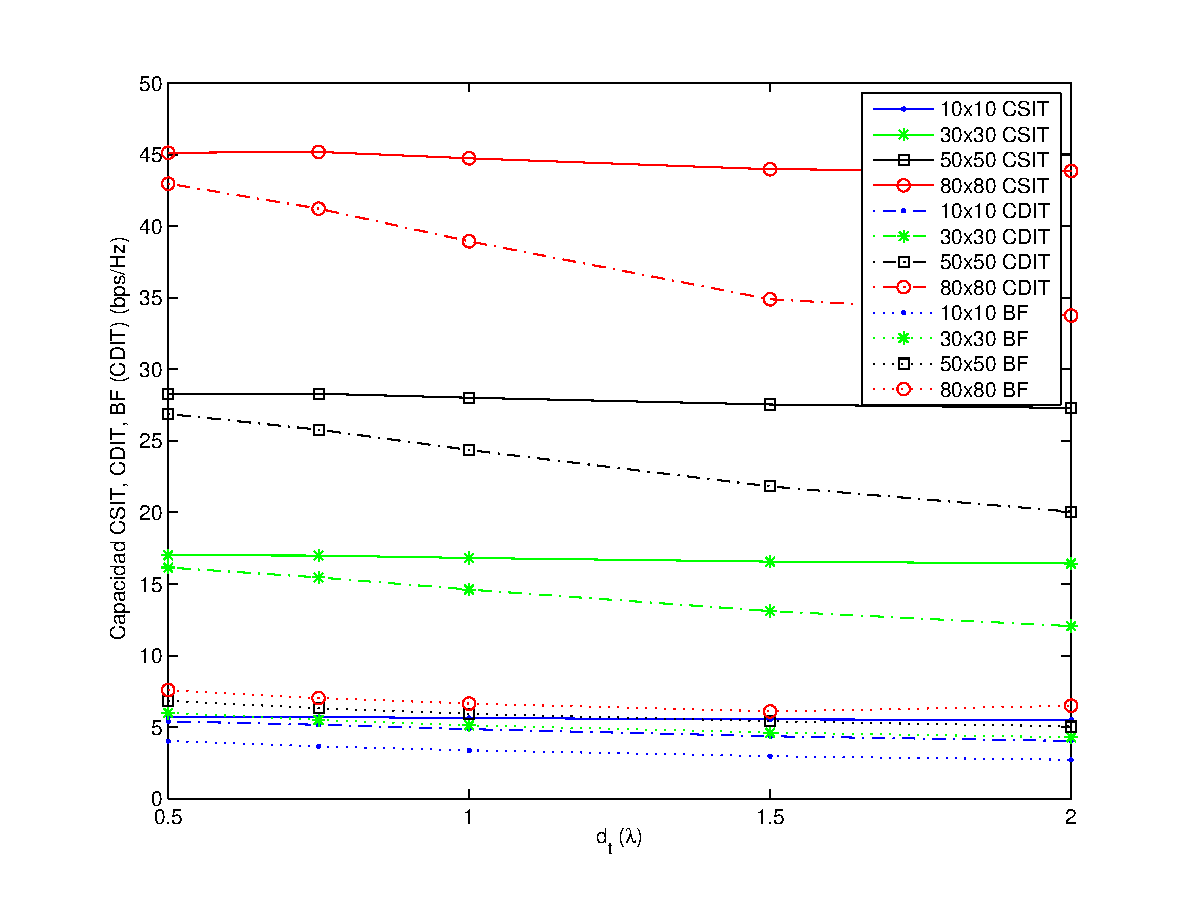
\includegraphics{figuras/CDIT_CSIT_SNRm5_ASD10.eps}}}}
	\mbox{ \subfigure[$ASD = 20^\circ$]{\resizebox{!}{10cm}		{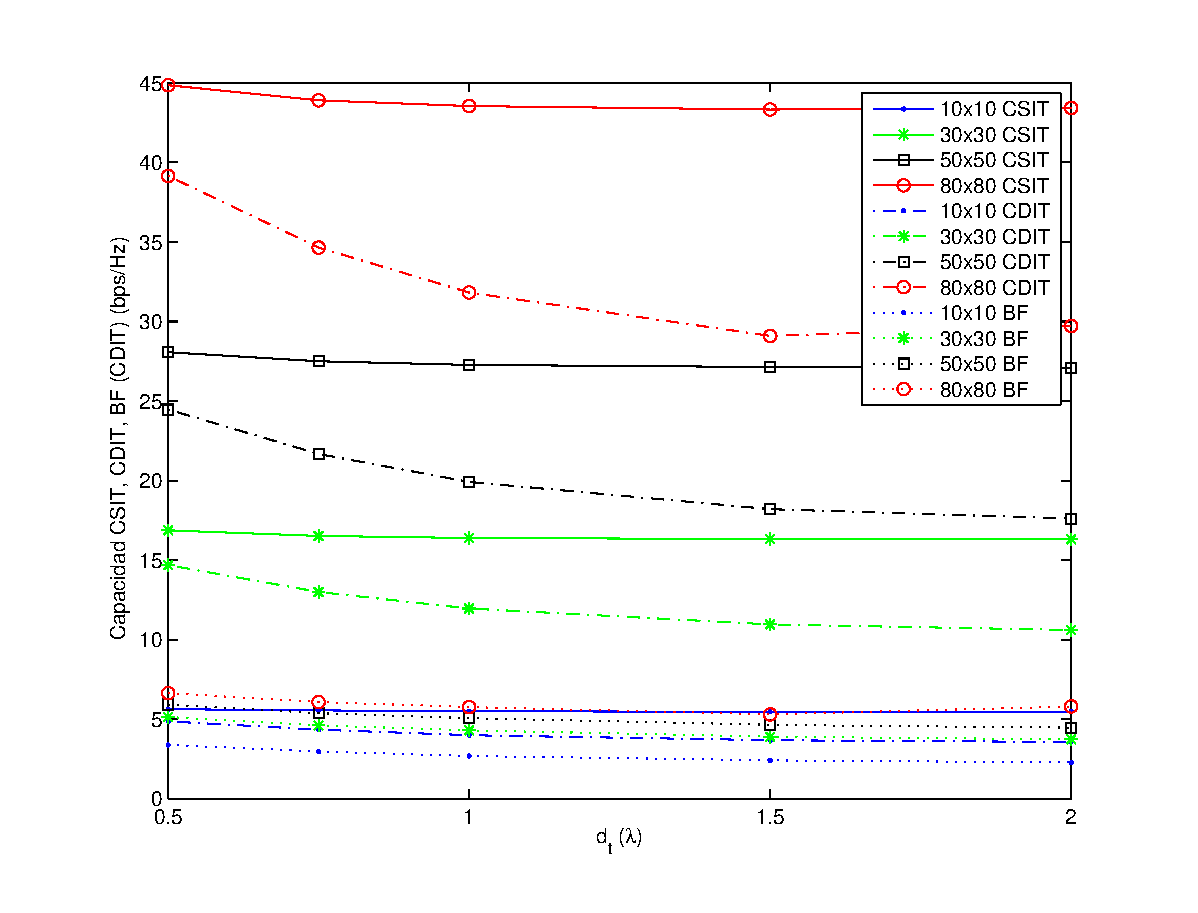
\includegraphics{figuras/CDIT_CSIT_SNRm5_ASD20.eps}}}}
	\caption{Comparaci�n de la capacidad en escenarios CSIT o CDIT (y diferenciando las dos estrategias de transmisi�n para este �ltimo) de un sistema MIMO Masivo con igual n�mero de antenas transmisoras y receptoras para $\snr = -5$ dB. Evoluci�n con respecto a la distancia entre antenas transmisoras.}
	\label{fig:MN_COMP_LS_DT}
\end{figure}


\begin{figure}
\centering
	\mbox{ \subfigure[$d_t = \frac{\lambda}{2}$]{\resizebox{!}{10cm}		{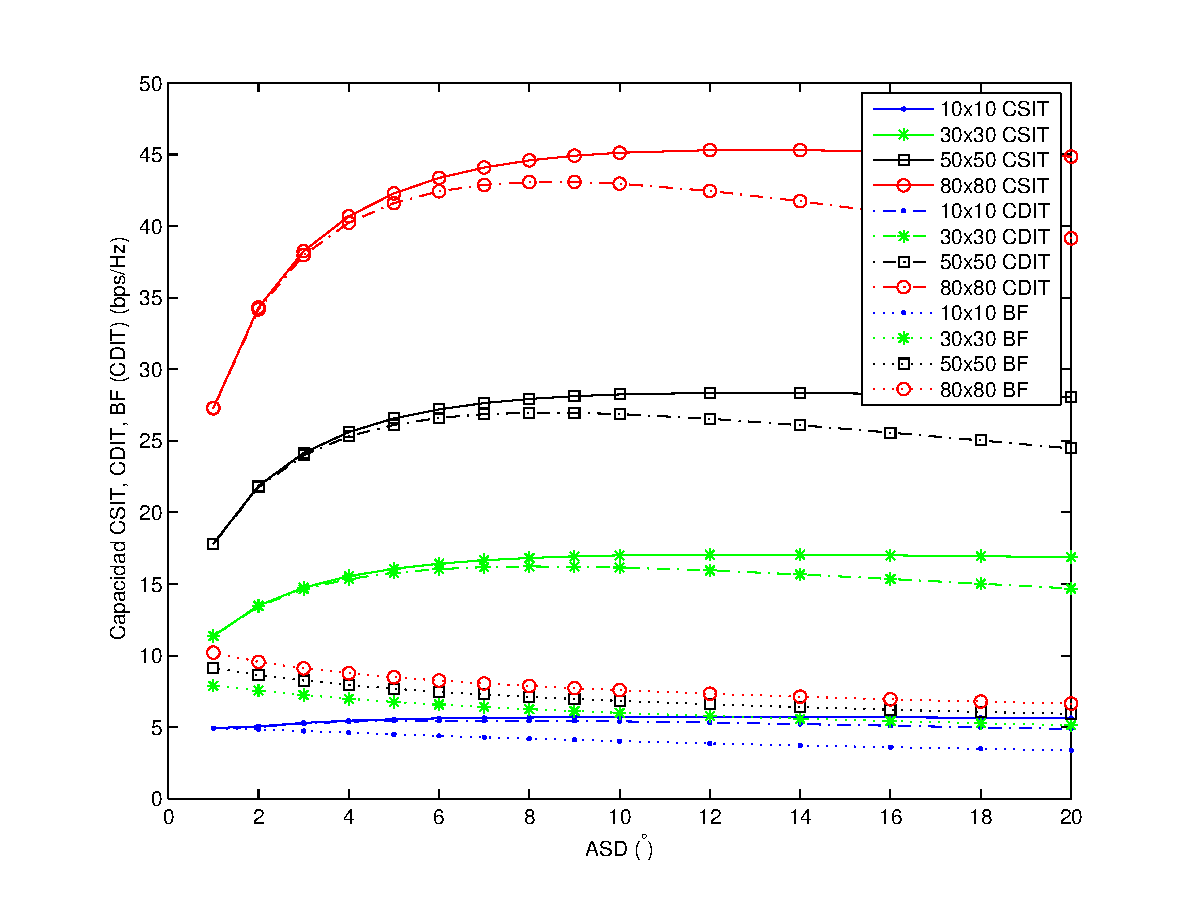
\includegraphics{figuras/CDIT_CSIT_SNRm5_dt05.eps}}}}
	\mbox{ \subfigure[$d_t = \lambda$]{\resizebox{!}{10cm}		{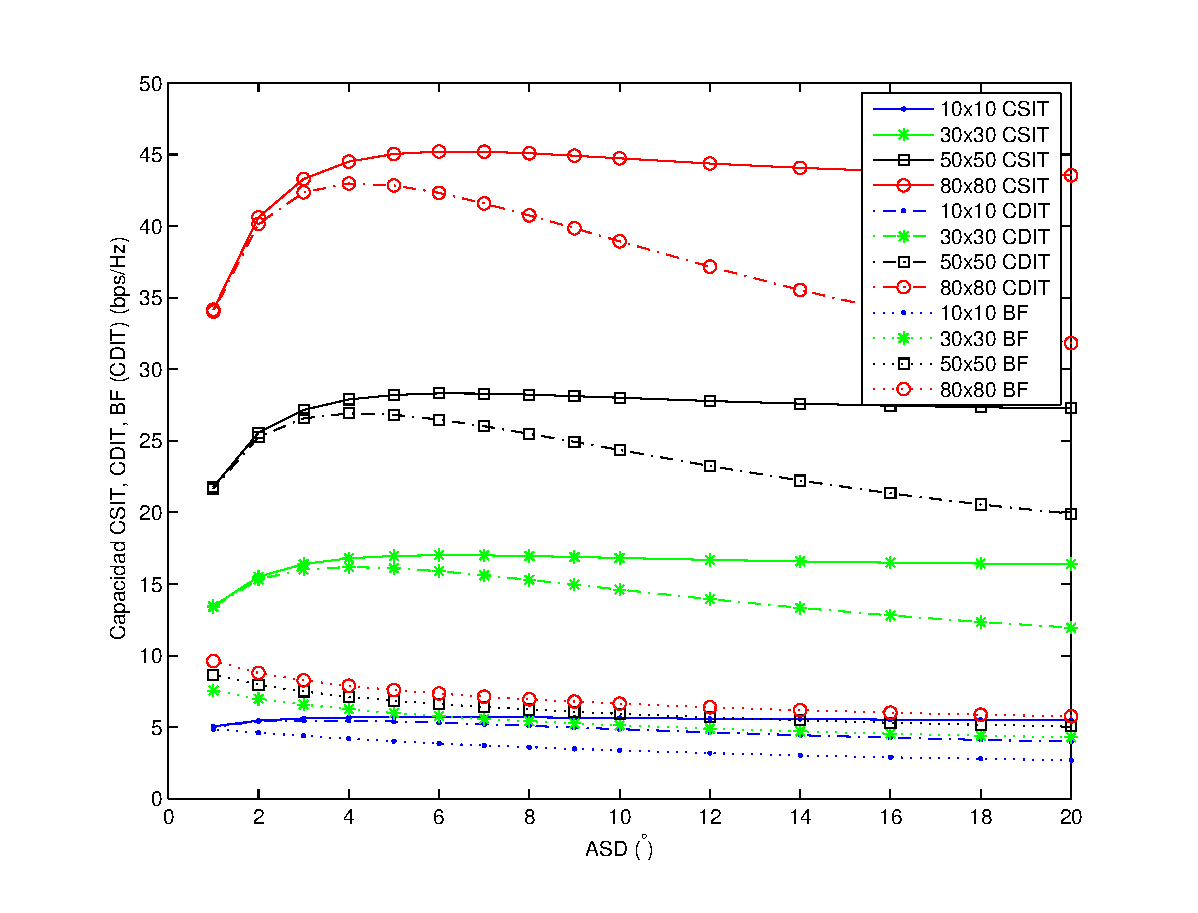
\includegraphics{figuras/CDIT_CSIT_SNRm5_dt1.eps}}}}
	\caption{Comparaci�n de la capacidad en escenarios CSIT o CDIT (y diferenciando las dos estrategias de transmisi�n para este �ltimo) de un sistema MIMO Masivo con igual n�mero de antenas transmisoras y receptoras para $\snr = -5$ dB. Evoluci�n con respecto al �ngulo de dispersi�n en el transmisor.}
	\label{fig:MN_COMP_LS_ASD}
\end{figure}

El comportamiento es similar al que coment�bamos en la secci�n anterior. Mientras que el algoritmo de Water-Filling empleado en el caso CSIT hace que  la capacidad se estabilice a partir de cierto valor de $d_t$ o $ASD$, los resultados de capacidad que arroja el caso CDIT se alejan cada vez m�s de los obtenidos para CSIT conforme aumentan tanto $d_t$ como $ASD$. Sin embargo, hemos encontrado un comportamiento que no esper�bamos en este caso, la existencia de un punto de trabajo para el que se alcanza la capacidad. Es decir, no nos acercamos m�s a la capacidad del sistema cuando la correlaci�n es m�s o menos alta sino que existe un punto concreto (muy apreciable en la figura (\ref{fig:MN_COMP_LS_ASD})) de $ASD$ para el cual la capacidad es m�xima. 

\subsubsection{Sistema MIMO masivo con M antenas transmisoras y 4 antenas receptoras}

En este �ltimo caso, la evoluci�n de las gr�ficas es la misma que la ya comentada. En las figuras (\ref{fig:MN_COMP_LS_DT_N4}) y (\ref{fig:MN_COMP_LS_ASD_N4}) se ve c�mo mientras el Water-Filling utilizado en el escenario CSIT tiende a estabilizarse a partir de cierto valor de $d_t$ o de $ASD$ (estabilizaci�n que suceder� antes cuando nos encontremos en condiciones con menor correlaci�n), la capacidad correspondiente al escenario CDIT disminuye a medida que la correlaci�n disminuye. 

\begin{figure}
\centering
	\mbox{ \subfigure[$ASD = 10^\circ$]{\resizebox{!}{10cm}		{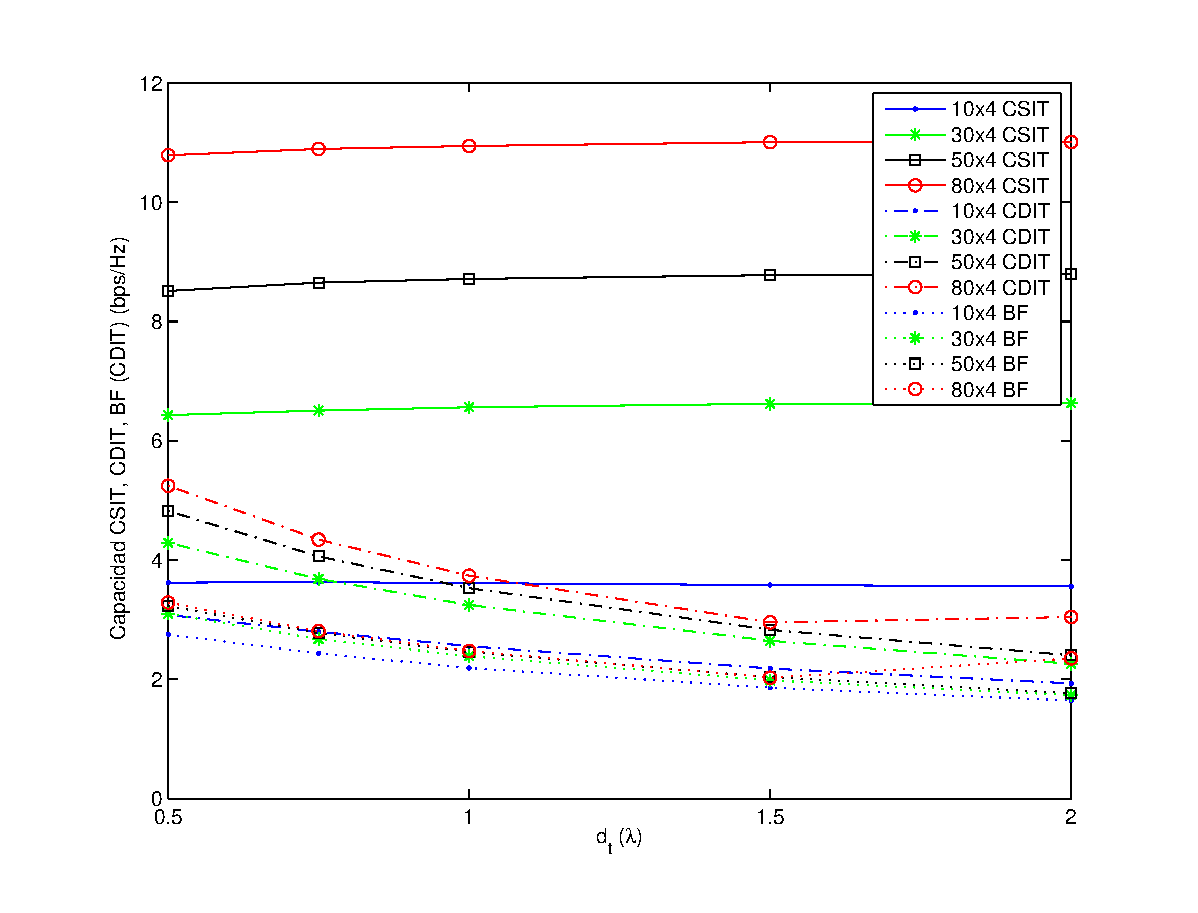
\includegraphics{figuras/CDIT_CSIT_SNRm5_ASD10_N4.eps}}}}
	\mbox{ \subfigure[$ASD = 20^\circ$]{\resizebox{!}{10cm}		{\includegraphics{figuras/CDIT_CSIT_SNRm5_ASD20_N4.eps}}}}
	\caption{Comparaci�n de la capacidad en escenarios CSIT o CDIT (y diferenciando las dos estrategias de transmisi�n para este �ltimo) de un sistema MIMO Masivo con $M$ antenas transmisoras y $4$ receptoras para $\snr = -5$ dB. Evoluci�n con respecto a la distancia entre antenas transmisoras.}
	\label{fig:MN_COMP_LS_DT_N4}
\end{figure}


\begin{figure}
\centering
	\mbox{ \subfigure[$d_t = \frac{\lambda}{2}$]{\resizebox{!}{10cm}		{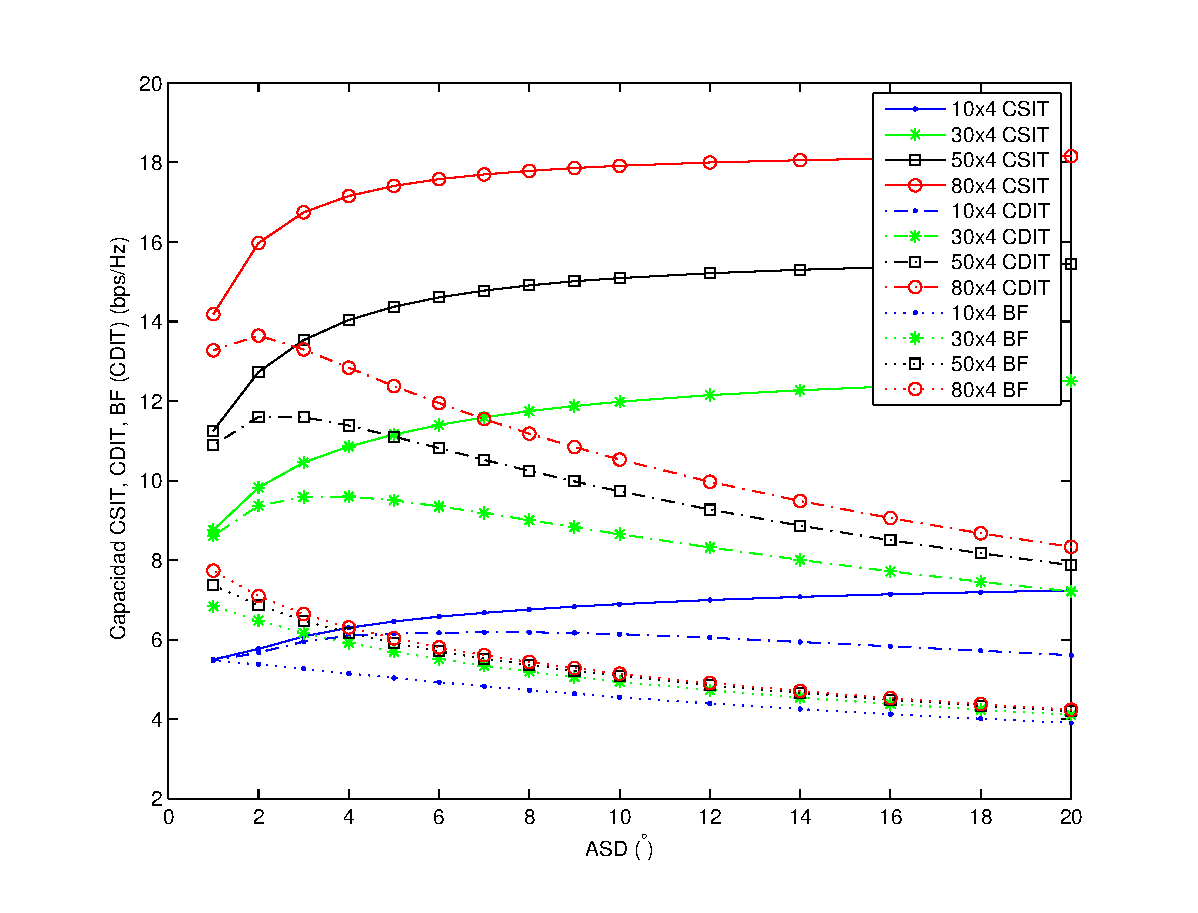
\includegraphics{figuras/CDIT_CSIT_SNRm5_dt05_N4.eps}}}}
	\mbox{ \subfigure[$d_t = \lambda$]{\resizebox{!}{10cm}		{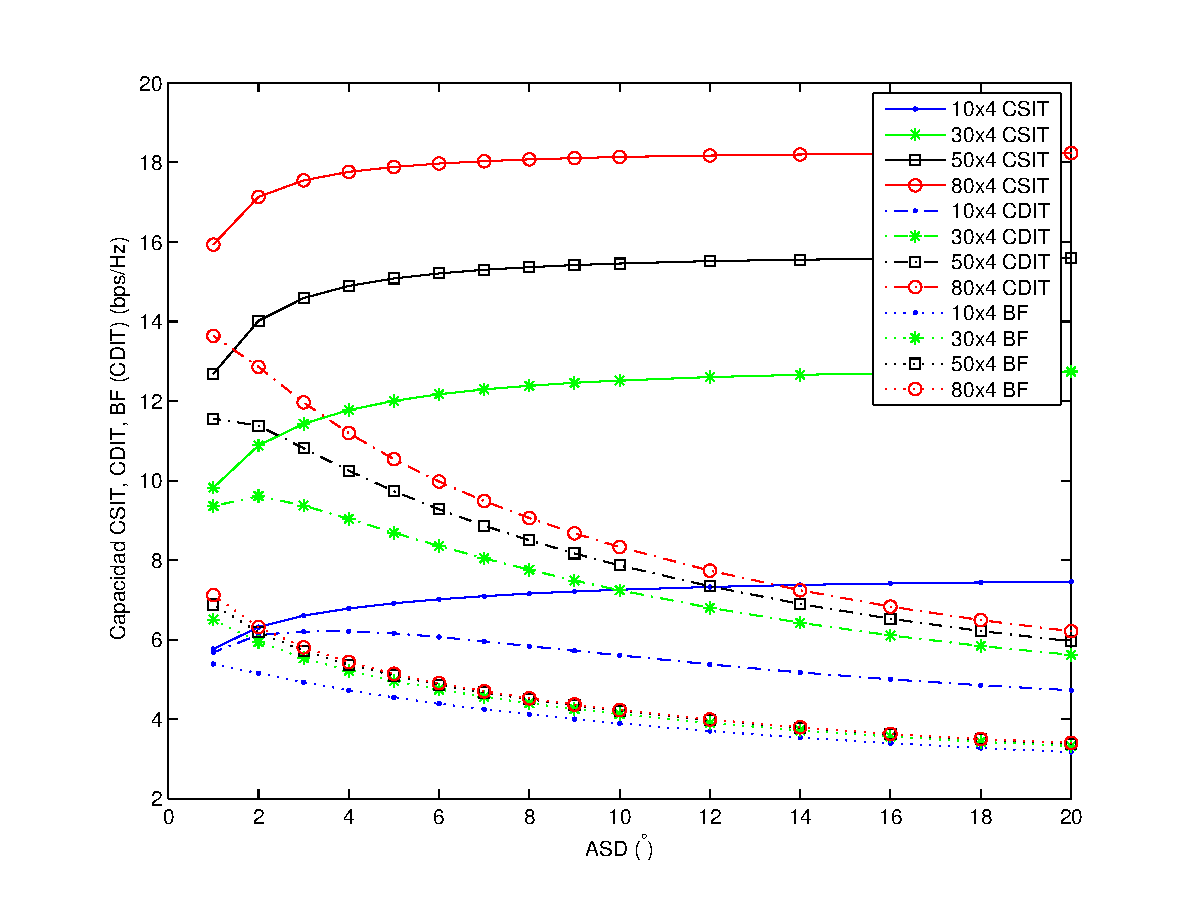
\includegraphics{figuras/CDIT_CSIT_SNRm5_dt1_N4.eps}}}}
	\caption{Comparaci�n de la capacidad en escenarios CSIT o CDIT (y diferenciando las dos estrategias de transmisi�n para este �ltimo) de un sistema MIMO Masivo con $M$ antenas transmisoras y $4$ receptoras para $\snr = -5$ dB. Evoluci�n con respecto al �ngulo de dispersi�n en el transmisor.}
	\label{fig:MN_COMP_LS_ASD_N4}
\end{figure}

\subsection{Comparaci�n entre los diferentes algoritmos para el escenario CDIT}\label{sec:comp}

Como ya hemos comentado en la secci�n \ref{sec:cdit}, para un escenario en el que existe CDIT, hemos implementado dos estrategias de transmisi�n diferentes. La primera de ellas trata de optimizar la matriz de covarianza en base a c�lculos a partir del m�nimo error cuadr�tico medio mientras que el segundo, mucho m�s sencillo, �nicamente inyecta toda la potencia en una de las antenas transmisoras. 

Como es de esperar, los resultados que obtendremos para el primero de ellos ser�n mejores que para el segundo. Se muestran estos resultados en las figuras (\ref{fig:comparacioncditbf}) y (\ref{fig:comparacioncditbf2}) donde, para una distancia entre antenas fija o un �ngulo de dispersi�n concreto, se puede comparar el comportamiento en t�rminos de capacidad que ofrece el beamforming generalizado frente al algoritmo de distribuci�n de potencia detallado anteriormente. 

\begin{figure}
\centering
	\mbox{ \subfigure[$d_t = \frac{\lambda}{2}$]{\resizebox{!}{7cm}		{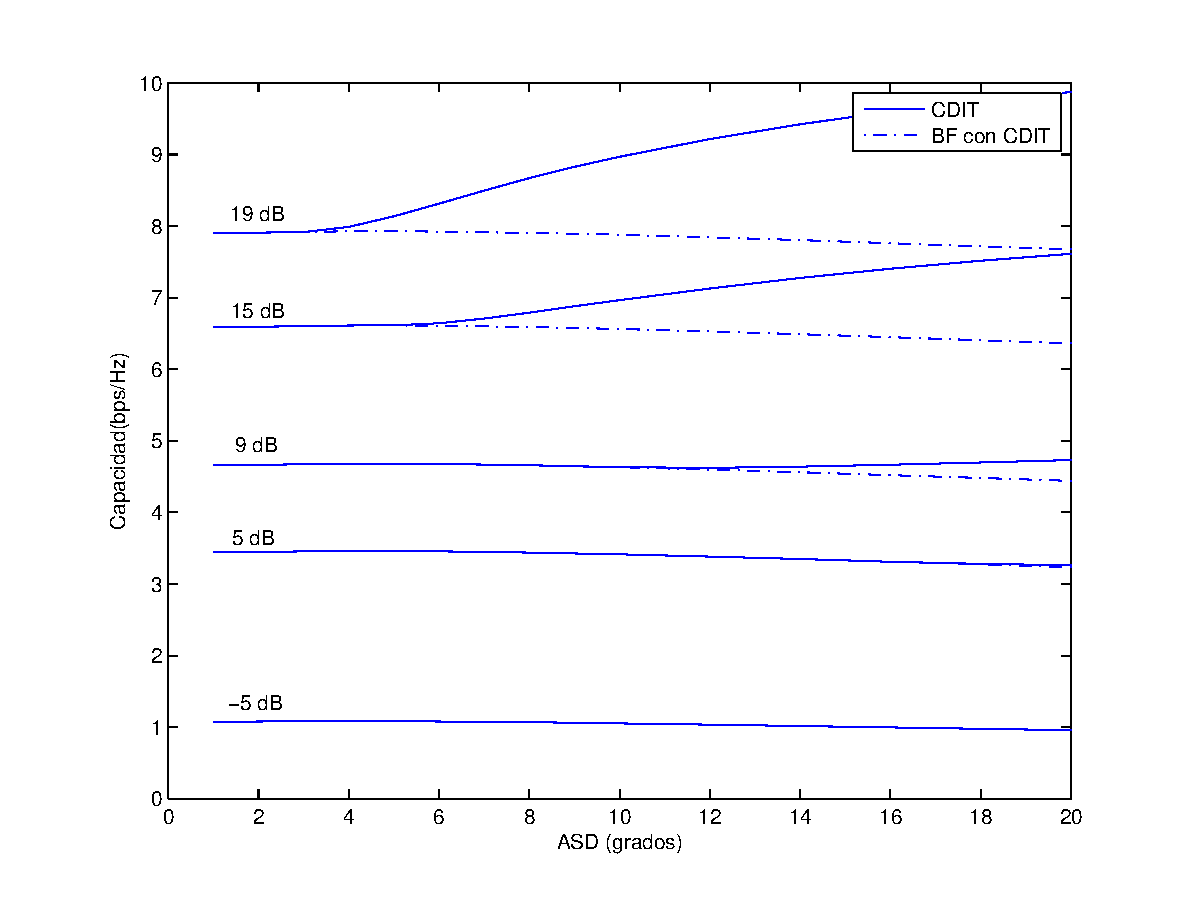
\includegraphics{figuras/comparacion_cdit_bf_M2_N2_dt05.eps}}}}
	\mbox{ \subfigure[$d_t = \lambda$]{\resizebox{!}{7cm}		{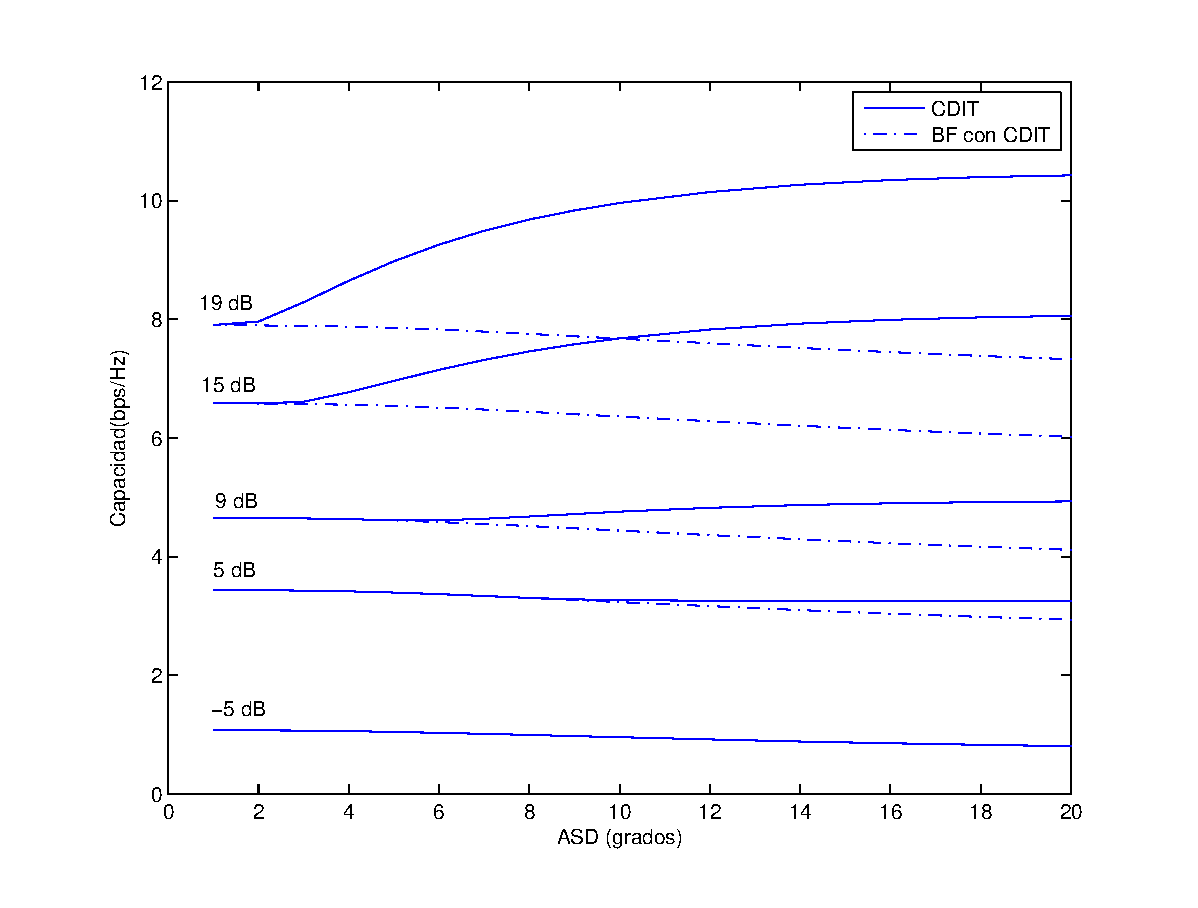
\includegraphics{figuras/comparacion_cdit_bf_M2_N2_dt1.eps}}}}
	\mbox{ \subfigure[$d_t = 2\lambda$]{\resizebox{!}{7cm}		{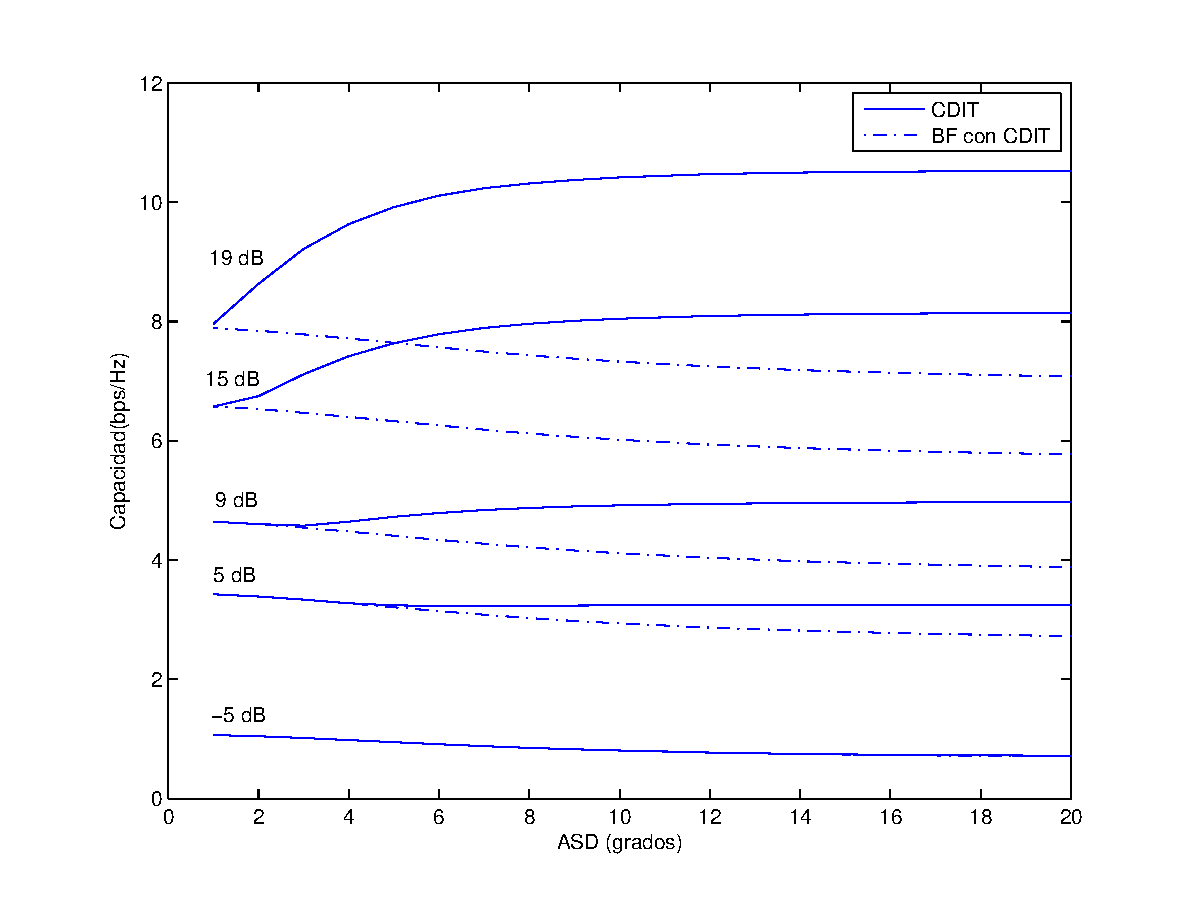
\includegraphics{figuras/comparacion_cdit_bf_M2_N2_dt2.eps}}}}
	\caption{Comparaci�n de las dos estrategias de transmisi�n planteadas para el escenario CDIT. Evaluaci�n de las mismas con respecto a $ASD$ y para diferentes valores de $\snr$}
	\label{fig:comparacioncditbf}
\end{figure}

\begin{figure}
\centering
	\mbox{ \subfigure[$ASD = 2^\circ$]{\resizebox{!}{7cm}		{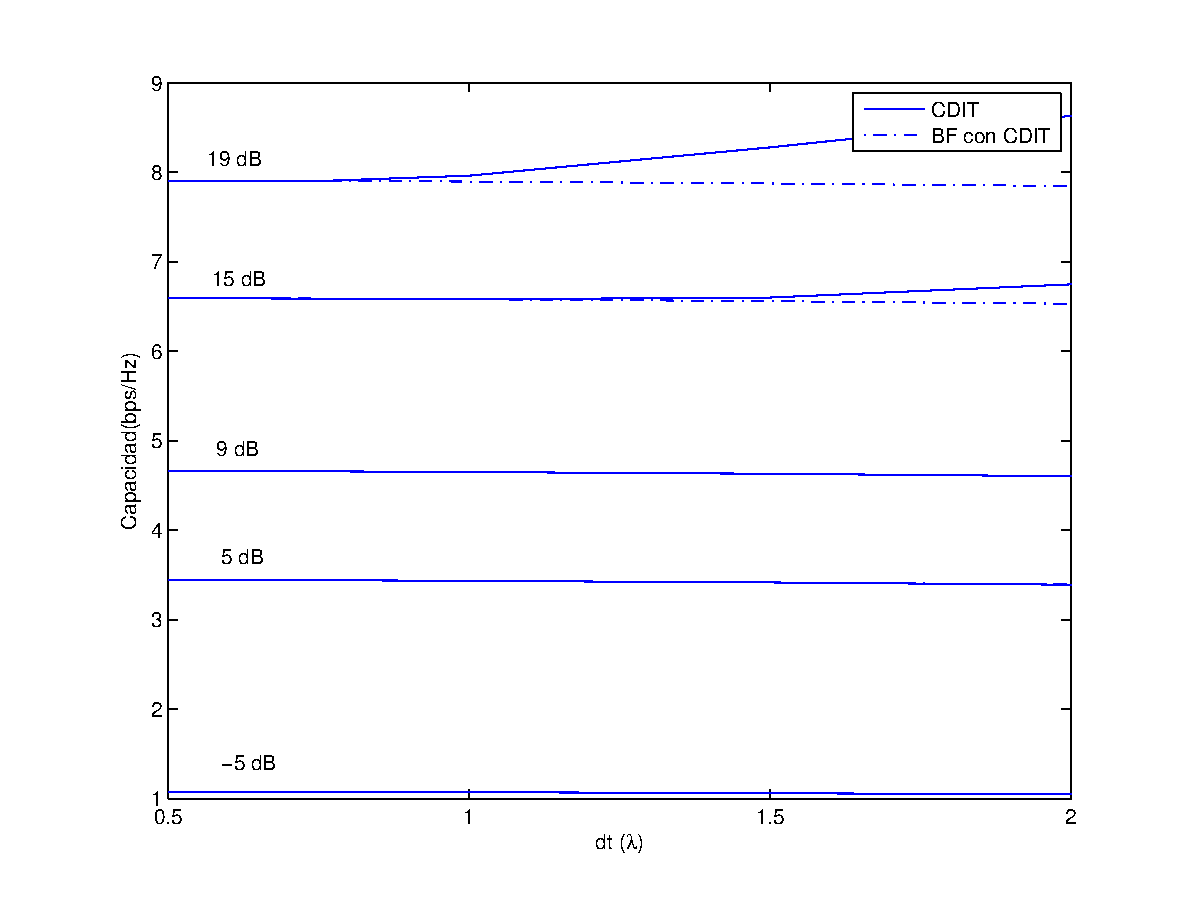
\includegraphics{figuras/comparacion_cdit_bf_M2_N2_ASD2.eps}}}}
	\mbox{ \subfigure[$ASD = 10^\circ$]{\resizebox{!}{7cm}		{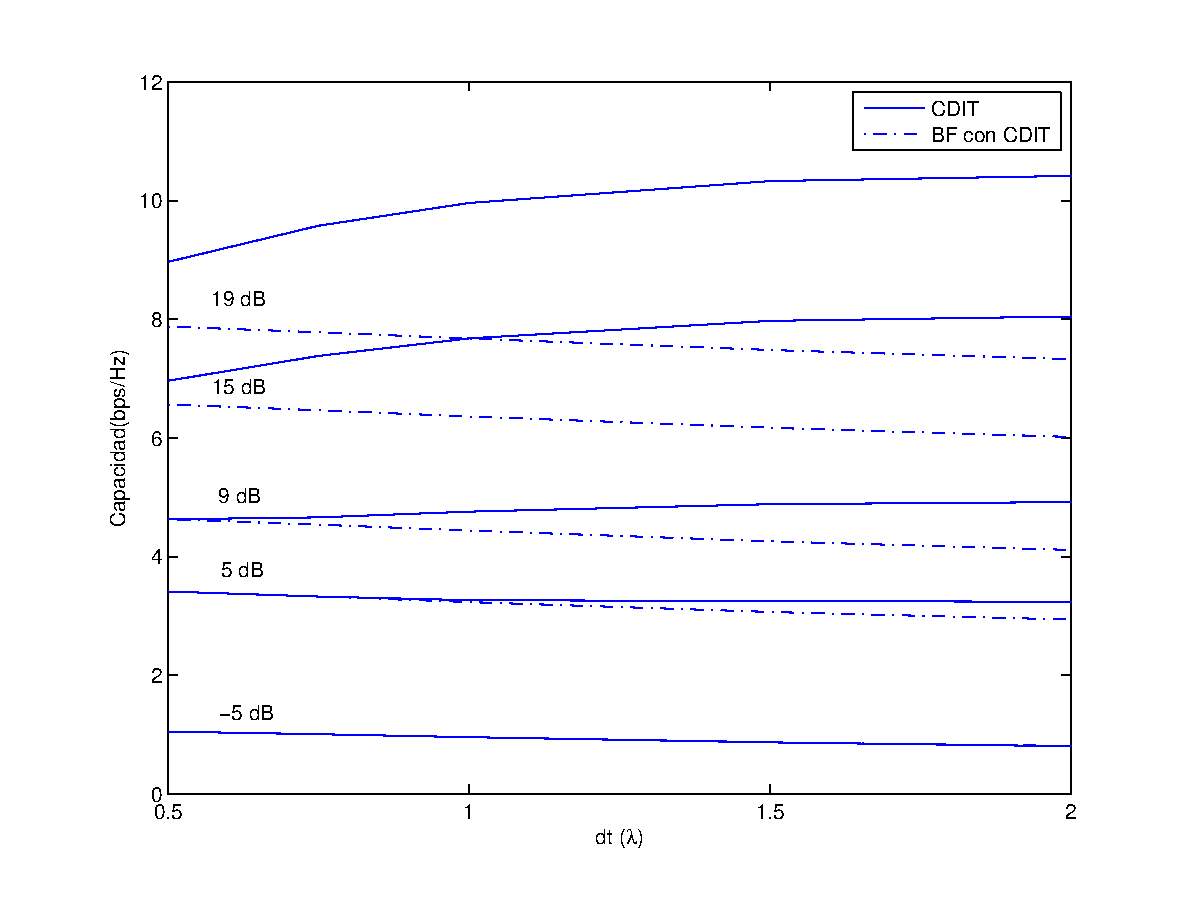
\includegraphics{figuras/comparacion_cdit_bf_M2_N2_ASD10.eps}}}}
	\mbox{ \subfigure[$ASD = 16^\circ$]{\resizebox{!}{7cm}		{\includegraphics{figuras/comparacion_cdit_bf_M2_N2_ASD16.eps}}}}
	\caption{Comparaci�n de las dos estrategias de transmisi�n planteadas para el escenario CDIT. Evaluaci�n de las mismas con respecto a $d_t$ y para diferentes valores de $\snr$}
	\label{fig:comparacioncditbf2}
\end{figure}

As�, tal y como anticip�bamos, en las figuras se puede apreciar c�mo el comportamiento de estas dos estrategias de transmisi�n para bajos niveles de SNR es pr�cticamente id�ntico. A medida que la $\snr$ va aumentando estos comportamientos se van alejando el uno del otro situ�ndose el beamforming como el peor de los dos. Adem�s, cuanto mayor es la $\snr$ antes empieza a ser �ptimo el algoritmo frente al beamforming. 

Cuando las condiciones en t�rminos de correlaci�n mejoran (es decir, aumenta la distancia entre antenas o la dispersi�n angular y por lo tanto disminuye la correlaci�n) tambi�n es posible ver c�mo el beamforming vuelve a ser peor que el algoritmo utilizado.

En resumen, las dos estrategias de transmisi�n arrojan resultados muy similares para entornos con bajos niveles de $\snr$ mientras que a medida que las condiciones se hacen favorables (aumenta la $\snr$, el $ASD$ o $d_t$) se hace notable la diferencia entre estas dos estrategias, posicion�ndose el beamforming como el peor de los dos. 
%%%%%%%%%%%%%%%%%%%%%%%%%%%%%%%%%%%%%%%%%%%%%%%%%%

%%%%%%%%%%%%%%%%%%%%%%%%%%%%%%%%%%%%%%%%%%%%%%%%%%
%%                  CAPITULO 4                  %%
%%%%%%%%%%%%%%%%%%%%%%%%%%%%%%%%%%%%%%%%%%%%%%%%%%
\chapter{Ortogonalidad}

Los sistemas MIMO masivo nos permiten desplegar un elevado n�mero de elementos en, al menos, uno de los dos extremos de la comunicaci�n. Uno de los aspectos clave que hace posible esta tecnolog�a es que la matriz de canal $\miH$ sea lo m�s ortogonal posible para simplificar as� el procesado de se�al. Dado que en este caso no estamos en escenarios con matrices de canal i.i.d. donde las matrices ser�an ortogonales, debemos encontrar una forma de medir esta ortogonalidad en los casos con los que estamos trabajando. En estos escenarios las premisas de las que partimos no son ideales sino que tienen m�ltiples limitaciones como un espacio limitado para el despliegue de las antenas o caracter�sticas del canal no deseadas.

Como ya hemos dicho nuestro inter�s reside en simplificar el procesado de se�al, uno de los cuellos de botella de los sistemas MIMO masivo debido a la complejidad del algoritmo asociado. El aspecto clave que hace posible esta simplificaci�n (que se traduce en una simplificaci�n del precodificador y el ecualizador) es la ortogonalidad. Si las filas o las columnas de la matriz de canal $\miH$ son ortogonales, ser� posible hacer uso de una estrategia de filtro adaptado en el transmisor y receptor. 

% *****************************************************************************************************************************
\section{Medidas de ortogonalidad}

Una matriz $\miA$ se dice que sus filas son ortogonales si
\begin{equation}
	\miA \miA^H = \mathbf{I}
\end{equation}
o que sus columnas son ortogonales si
\begin{equation}
	\miA^H \miA = \mathbf{I}
\end{equation}
que se traduce en
\begin{equation}
	\miA^{-1} = \miA^H
\end{equation}
donde $\miA^H$ es la matriz transpuesta, e $\mathbf{I}$ es la matriz identidad. Esta propiedad hace que trabajar con matrices ortogonales sea especialmente f�cil, ya que hallar la matriz transpuesta de $\miA$ es mucho m�s sencillo que hallar su inversa. 

Volviendo a nuestro escenario, en el que el canal queda definido por la matriz $\miH$, lo que buscamos es que esta matriz sea lo m�s ortogonal posible, dado que esto simplificar�a enormemente el procesamiento de se�al. Sabiendo que el lugar m�s factible para desplegar muchas antenas es la BS (estaci�n base), podemos dise�ar un precodificador o un ecualizador muy simple para el caso del enlace descendente o ascendente, respectivamente. En ambos casos ser�a un filtro adaptado. 

Nos centraremos en el caso del enlace descendente, por lo que matem�ticamente la propiedad que buscamos en nuestra matriz de canal $\miH$ es
\begin{equation}
	\frac{\miH\miH^H}{M}\approx \mathbf{I}_N
\end{equation}
es decir, buscamos que las filas de $\miH$ sean ortogonales. 

%\begin{Triple m�ximo}
Cada elemento $h_{nm}$ caracteriza el canal existente entre la antena $m$-�sima transmisora y la antena $n$-�sima receptora; cada fila entonces de la matriz $\miH$ caracterizar� el canal entre las $M$ antenas transmisoras y la antena $n$-�sima receptora. Nos interesa que cada fila $[h_{1m}\text{ }  h_{2m}\text{ }... \text{ }h_{NM}]$ sea ortogonal al resto de filas, es decir, independiente a las comunicaciones que viajan a otra antena receptora. 
%\end{Triple m�ximo}

Para medir el nivel de ortogonalidad de la matriz $\miH$, es necesario definir una medida para esta magnitud. Proponemos a continuaci�n varias medidas con las que hemos trabajado, para despu�s concluir con la que nos parece m�s adecuada y por qu�. Para evaluar su comportamiento lo haremos observando los resultados de las medidas explicadas a continuaci�n comparando en cada caso el comportamiento para las matrices de canal $M \times 2$, $M \times 4$, $M \times M$ e i.i.d.

\subsection{Norma de Frobenius}\label{theo_frobenius}

En este primer caso, utilizamos el concepto de norma matricial (Anexo \ref{anexo}) y en particular el caso concreto de normas componente a componente, definidas como:
\begin{equation}
	{\left\|A\right\|}_p = \left(\sum_{i = 1}^{M}\sum_{j = 1}^{N}|a_{ij}|^p\right)^{1/p}
\end{equation}
Para $p = 2$, a esto se le llama norma de Frobenius o norma de Hilbert-Schmidt. La norma de Frobenius es una norma matricial que se define como la ra�z cuadrada de la suma de los valores absolutos de los elementos que forman la matriz $\miA$ de dimensiones $M \times N$
\begin{equation}
	{\left\|A\right\|}_F = \sqrt{\sum_{i = 1}^{M}{\sum_{j = 1}^{N}|a_{ij}|^2}}
\end{equation}
La norma de Frobenius tambi�n equivale a la ra�z cuadrada de la traza de la matriz $\miA\miA^H$, donde $\miA^H$ es la matriz transpuesta conjugada, 
\begin{equation}
	{\left\|A\right\|}_F = \sqrt{Tr(\miA\miA^H)}
\end{equation}

Utilizaremos esta norma para calcular la distancia que existe entre la matriz $\frac{\miH\miH^H}{M}$ y la matriz identidad $\mathbf{I}_N$. Definimos as� nuestra medida como

\begin{equation}
d\left(\frac{\miH\miH^H}{M}, \mathbf{I}_N\right) = {\left \|   \frac{\miH\miH^H}{M} - \mathbf{I}_N  \right\|}_F
\end{equation}


\subsection{Defecto de ortogonalidad }\label{theo_lattice}

El defecto de ortogonalidad es una medida de lo cerca que est� una matriz de ser ortogonal, partiendo del concepto de bases de vectores ortogonales que forman un espacio. Compara el producto de la longitud de los vectores que forman la base con el volumen del paralelep�pedo que definen. Para una base formada por vectores perfectamente ortogonales, estas dos cantidades deber�an ser iguales. 

Cualquier base de $n$ vectores puede ser representada por la matriz $\miA$, cuyas columnas son los vectores de la base $a_i, i = 1, ..., n$. Cuando el n�mero de vectores que forman la base es igual a la dimensi�n del espacio que ocupan, la matriz $\miA$ es cuadrada, y el volumen del paralelep�pedo es simplemente el valor absoluto del determinante de la matriz, $\det(\miA)$. Si el n�mero de vectores de la base es menor a la dimensi�n del espacio, el volumen queda definido por $\sqrt{\det(\miA^H\miA)}$. 

Se define entonces el defecto de ortogonalidad como
\begin{equation}
	\delta(\miA) = \frac{\prod_{i = 1}^{n}\|a_i\|}{\sqrt{det(\miA^H\miA)}}
\end{equation}

De la definici�n geom�trica se deriva que $\delta(\miA) \geq  1$ y �nicamente en el caso de que la base sea ortogonal tendremos $\delta(\miA) = 1$. 

Nosotros aplicaremos esta medida a nuestra matriz de canal $\miH$, buscando ortogonalidad en las filas por lo que la expresi�n final queda de la siguiente forma:
%%%%%-----mMIRAAAAAAAAAAR!!!!!
\begin{equation}
	\delta(\miA) = \frac{\prod_{i = 1}^{n}\|h_i\|}{\sqrt{det(\miH\miH^H)}}
\end{equation}

donde $\|h_i\|$ son las filas de $\miH$.


\subsection{Norma del producto de las filas}\label{theo_prod}

En tercer lugar, hemos hecho uso de la propiedad de que el producto escalar de dos vectores ortogonales es nulo. Si una matriz $\miA$ tiene las columnas ortogonales, el producto de una columna por cualquier otra ser� tambi�n cero. 

As�, hemos definido la siguiente medida de ortogonalidad que calcula la suma de los valores absolutos del producto de una fila por el resto (recordemos que nosotros buscamos que las filas de $\miH$ sean ortogonales)
\begin{equation}
	\Lambda = \sum_{i = 1}^{N}\sum_{j = 1\\j \neq i}^N |a_i^Ha_j|
\end{equation}

De esta forma, cuanto m�s cerca de 0 est� $\Lambda$ m�s cerca estaremos de la ortogonalidad

\subsection{Elecci�n de la medida de ortogonalidad m�s adecuada}

Para escoger la medida que m�s se adapta a lo que buscamos, compararemos los resultados que nos ofrece cada una de ellas para diferentes casos i.i.d.. Para un n�mero $M$ concreto de antenas en el transmisor, obtendremos los resultados de ortogonalidad con $2$, $4$ o $M$ antenas en el receptor. 

En primer lugar, en la tabla (\ref{tabla_frobe}) se puede observar el comportamiento de la \textbf{norma de Frobenius} (detallada en la secci�n \ref{theo_frobenius})para el caso de $M = 50$ y diferentes antenas en el receptor. 

\begin{table}[htb]
\centering
\begin{tabular}{|c|c|}
  \hline
  \multicolumn{2}{|c|}{Norma de Frobenius para $M = 50$} \\
  \hline
  $N = 2$ & 0.2625 \\
  $N = 4$ & 0.5530 \\
  $N = 50$ & 7.0633 \\
  \hline
\end{tabular}
\caption{Valores de la norma de Frobenius para el caso de matrices i.i.d. con 50 antenas en el transmisor y 2, 4 y 50 antenas en el receptor}
\label{tabla_frobe}
\end{table}


Intuitivamente, se podr�a creer que el nivel de ortogonalidad que deber�amos obtener para todas las matrices i.i.d deber�a ser el mismo pero como vemos en las gr�ficas no lo es. Para entender esta propiedad basta con observar que calcular la norma de Frobenius de matriz se reduce a calcular la suma de los valores absolutos de cada elemento de la matriz. Una matriz de mayor tama�o tendr� m�s elementos y por tanto su norma de Frobenius ser� necesariamente mayor. Es por esto que los valores correspondientes a los casos de 50x2 o 50x4 se encuentran pr�ximos a cero pero el de 50x50 se encuentra por encima, alrededor de un valor de 7. 

En cuanto al \textbf{defecto de ortogonalidad} explicado en la secci�n \ref{theo_lattice}, en la tabla \ref{tabla_lattice} encontramos los valores que arroja esta medida para los mismos casos evaluados con la norma de Frobenius. De nuevo para $N = 2$ y $N = 4$ obtenemos valores muy bajos pero, con $N = 50$, el resultado se dispara enormemente. 

\begin{table}[htb]
\centering
\begin{tabular}{|c|c|}
  \hline
  \multicolumn{2}{|c|}{Defecto de ortogonalidad para $M = 50$} \\
  \hline
  $N = 2$ & 1.0386 \\
  $N = 4$ & 1.2740\\
  $N = 50$ & 3.9085 x $10^{30}$ \\
  \hline
\end{tabular}
\caption{Valores del defecto de ortogonalidad para el caso de matrices i.i.d. con 50 antenas en el transmisor y 2, 4 y 50 antenas en el receptor}
\label{tabla_lattice}
\end{table}

Por �ltimo, en cuanto a la tercera medida comentada en la secci�n \ref{theo_prod}, los valores obtenidos los podemos encontrar el la tabla \ref{tabla_producto}. Pese a que el valor obtenido para $N = 2$ es muy bajo, el crecimiento que sufre esta medida con respecto a $N$ es bastante r�pido, y ya para $N = 4$ nuestra medida nos ofrece un resultado de 3.0936. En el caso de $N = 50$ el aumento de este valor es muy grande, alcanzando el valor de 955.8792. Dado que nuestra matriz $\miH$ (i.i.d. en este caso) ha sido generada de forma aleatoria, la probabilidad de que dos filas de $\miH$ sean independientes es mucho m�s alta que la probabilidad de que 50 filas lo sean, y de ah� que el resultado que nos da la medida de ortogonalidad para dimensiones elevadas sea mucho mayor y, por tanto, denote menor ortogonalidad

\begin{table}[htb]
\centering
\begin{tabular}{|c|c|}
  \hline
  \multicolumn{2}{|c|}{Producto de filas para $M = 50$} \\
  \hline
  $N = 2$ & 0.4999 \\
  $N = 4$ & 3.0936\\
  $N = 50$ & 955.8792\\
  \hline
\end{tabular}
\caption{Valores del producto de filas para el caso de matrices i.i.d. con 50 antenas en el transmisor y 2, 4 y 50 antenas en el receptor}
\label{tabla_producto}
\end{table}

Una vez comparados los resultados de las tres medidas de ortogonalidad propuestas, estamos ya en condiciones de seleccionar aquella que m�s se adapta a lo que buscamos para realizar las simulaciones. Nuestro objetivo es encontrar aquella medida que nos d� resultados similares de ortogonalidad para los tres casos i.i.d. estudiados. En los tres escenarios observamos c�mo los valores para los casos de dimensiones reducidas ($N = 2$ y $N = 4$) son suficientemente bajos, aumentando a medida que las dimensiones aumentan. De las tres medidas analizadas, aquella que sufre un crecimiento menor con respecto a la dimensi�n es la norma de Frobenius, por lo que la elegiremos como la m�s adecuada y haremos uso de ella en las simulaciones sucesivas. Adem�s, esta medida de ortogonalidad es consistente con la que se propone en \cite{tensor}




% *****************************************************************************************************************************

\section{Resultados de ortogonalidad de las simulaciones}\label{cap:seccion_simul}

\subsection{Par�metros de las simulaciones}

Los par�metros que emplearemos en estas simulaciones ser�n los mismos que describimos en la secci�n \ref{sec:param}.


\subsection{Ortogonalidad en el caso asim�trico $N = 2$}\label{cap:orto_N2}

Se muestran en esta secci�n los resultados de ortogonalidad obtenidos para un escenario en el que $N = 2$. Para ello, asumimos un escenario incorrelado en el receptor que podr�a tratarse o bien en un sistema MIMO multiusuario en el que la BS sirve a 2 usuarios o bien en un sistema de un �nico usuario con 2 antenas en el receptor. 

En la figura (\ref{fig:orto2}) podemos observar el efecto que produce la distancia entre antenas transmisoras $d_t$ en la ortogonalidad de $\miH$. En ellas se puede ver c�mo a mayor distancia entre antenas mejor es el nivel de ortogonalidad obtenido, lo que deriva inevitablemente en la necesidad de mayor espacio f�sico para el despliegue de las antenas. 

\begin{figure}[htbp]
\centering
	\mbox{ \subfigure[$ASD = 5^\circ$]{\resizebox{!}{7cm}		{\includegraphics{figuras/orto_barridoM_N2_ASD5}}}}
	\mbox{ \subfigure[$ASD =10^\circ$]{\resizebox{!}{7cm}		{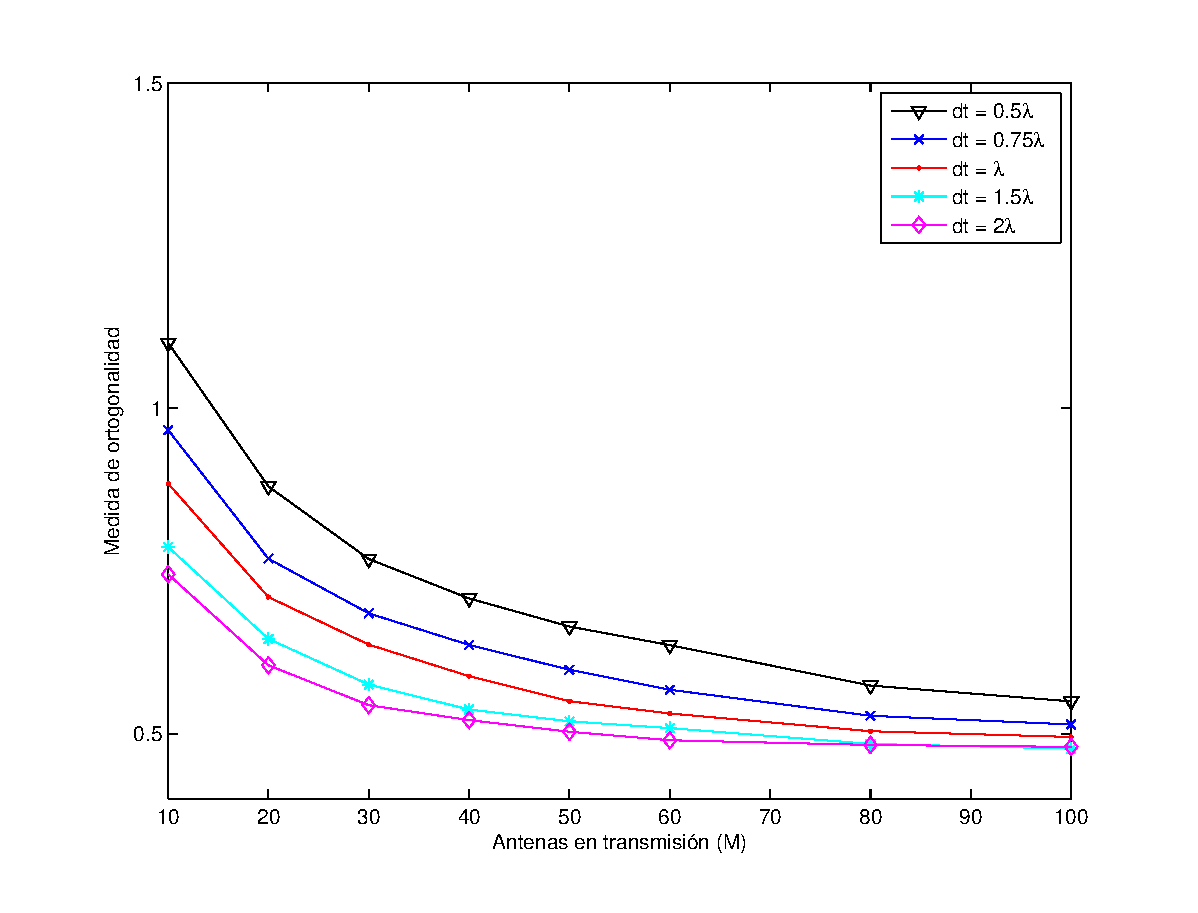
\includegraphics{figuras/orto_barridoM_N2_ASD10}}}}
	\mbox{ \subfigure[$ASD =20^\circ$]{\resizebox{!}{7cm}		{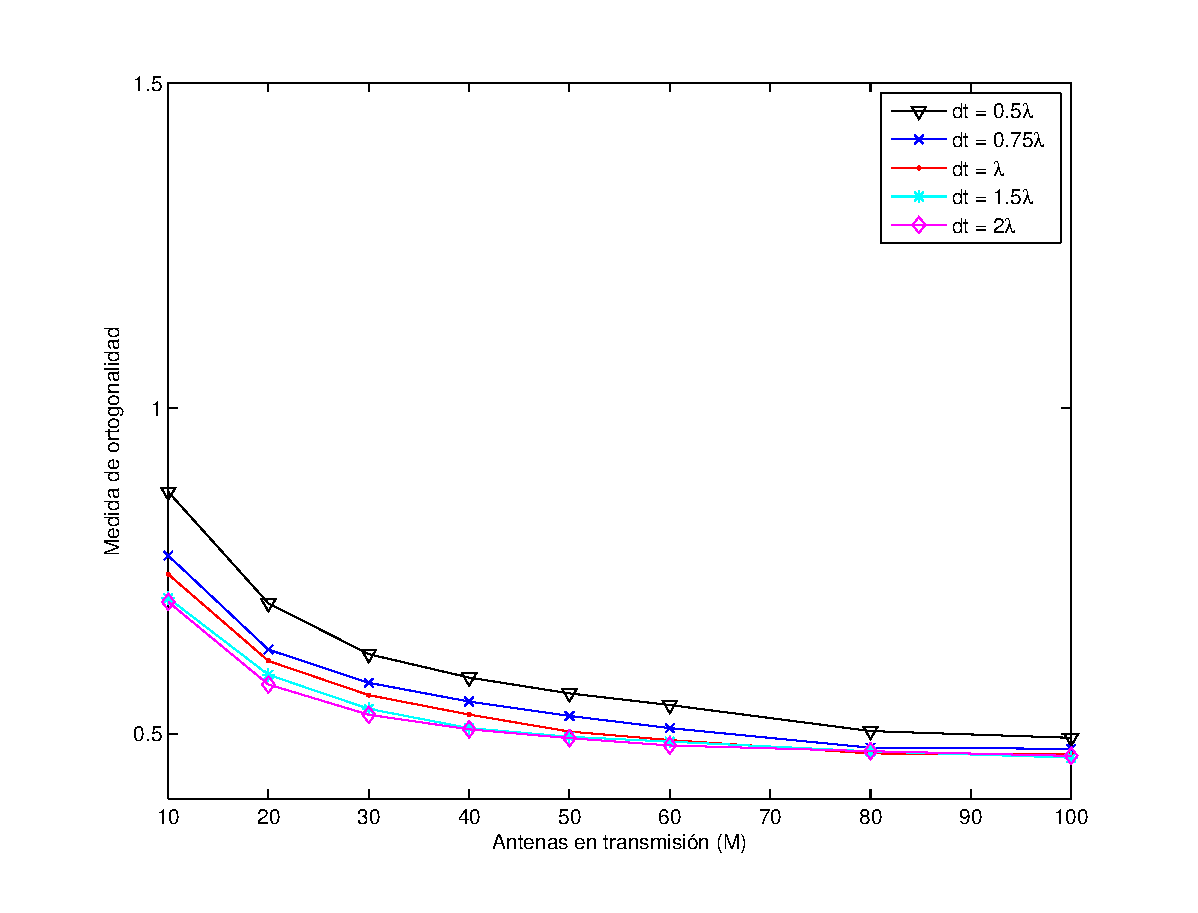
\includegraphics{figuras/orto_barridoM_N2_ASD20}}}}
	\caption{Medida de ortogonalidad para un sistema MIMO masivo con $M$ antenas transmisoras y $2$ antenas receptoras para diferentes valores de $d_t$.}
	\label{fig:orto2}
\end{figure}

Adem�s, podemos observar un efecto de saturaci�n en las gr�ficas en relaci�n al valor de $M$. Llega un punto en el que la mejora que provoca un aumento del n�mero de antenas en transmisi�n ($M$) es m�nima. A valores bajos de $M$, aumentar el n�mero de antenas transmisoras mejora significativamente la ortogonalidad de la matriz. Para valores elevados, a partir de entre 50 y 60 antenas transmisoras, esta mejora no es significativa y probablemente habr�a que analizar el coste f�sico del despliegue del sistema para estudiar si merecer�a la pena incluir tantas antenas. Este efecto se hace m�s pronunciado cuanto mayor es el valor de ASD, es decir, cuando nos encontramos en condiciones m�s favorables antes aparece el efecto de saturaci�n. A medida que disminuye ASD, las matrices realistas tienden de forma m�s lenta a una mayor ortogonalidad y existe mayor distancia entre la medida calculada a diferentes valores de $d_t$ (por ejemplo, la diferencia que existe en la ortogonalidad para la matriz correspondiente a $d_t = 0.75\lambda$ y a $dt_t = \lambda$ es mayor para $ASD = 5^\circ$ que para $ASD = 20^\circ$). 

\begin{figure}[htbp]
\centering
	\mbox{ \subfigure[$d_t = 0.5\lambda$]{\resizebox{!}{7cm}		{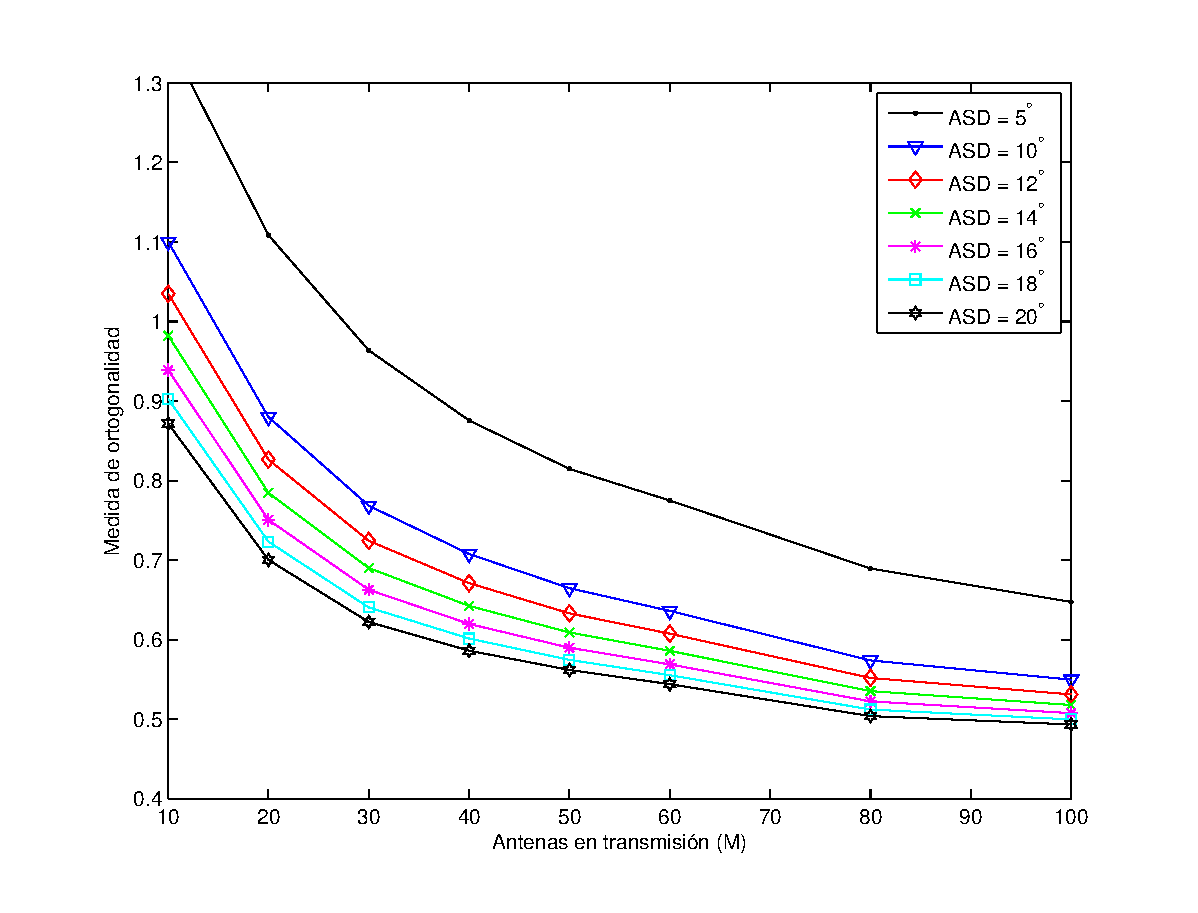
\includegraphics{figuras/orto_barridoM_N2_dt05}}}}
	\mbox{ \subfigure[$d_t = \lambda$]{\resizebox{!}{7cm}		{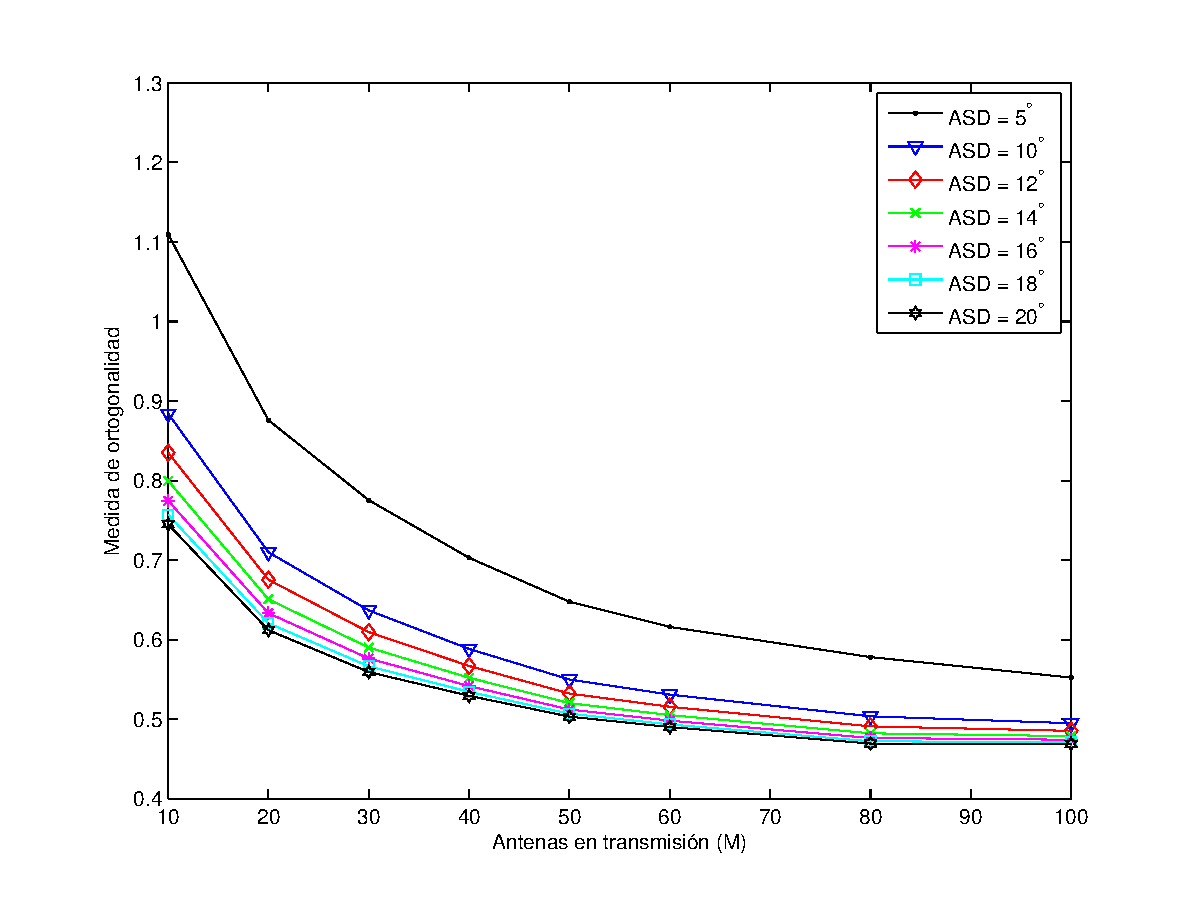
\includegraphics{figuras/orto_barridoM_N2_dt1}}}}
	\mbox{ \subfigure[$d_t = 2\lambda$]{\resizebox{!}{7cm}		{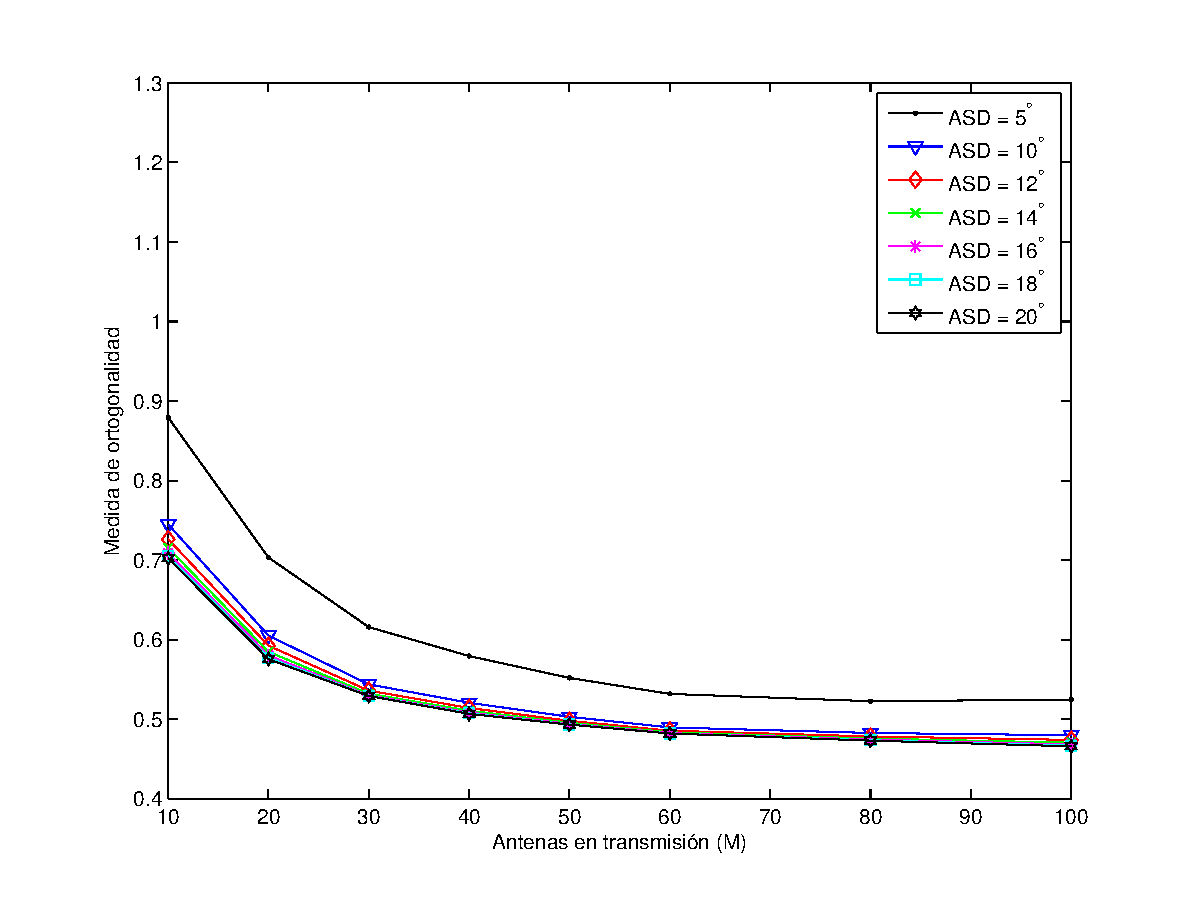
\includegraphics{figuras/orto_barridoM_N2_dt2}}}}
	\caption{Medida de ortogonalidad para un sistema MIMO masivo con $M$ antenas transmisoras y $2$ antenas receptoras para diferentes valores de $ASD$.}
	\label{fig:orto2_dt}
\end{figure}


De la figura (\ref{fig:orto2_dt}) que muestra el comportamiento de la ortogonalidad de $\miH$ con respecto a diferentes valores de ASD, podemos extraer conclusiones similares. Al igual que antes prefer�amos casos en los que la distancia entre antenas transmisoras fuera lo mayor posible, tambi�n ahora nos interesa un valor de ASD lo mayor posible. Cuanto m�s peque�a sea la dispersi�n angular, la distancia obtenida entre $\miH$ y la matriz identidad ser� mayor y por tanto, nuestra $\miH$ ser� menos ortogonal. 

De nuevo aparece el efecto de saturaci�n ya comentado anteriormente. Para valores peque�os de $M$, a�adir m�s antenas en el transmisor mejora significativamente la ortogonalidad. No sucede esto mismo a partir de valores elevados de $M$ (alrededor de 50 o 60), cuando se produce este efecto de saturaci�n y no mejora demasiado la ortogonalidad. Dicho efecto sucede antes para valores altos de $d_t$. 

\subsection{Ortogonalidad en el caso asim�trico $N = 4$}

Continuando en un escenario MIMO masivo con $M$ antenas en transmisi�n y $N = 4$ antenas en recepci�n, las simulaciones en este caso nos arrojan comportamientos de la matriz $\miH$ pr�cticamente id�nticos a los obtenidos para $N = 2$. Para ilustrarlo, s�lo incluiremos la gr�fica (\ref{fig:orto4}) que muestra los resultados para $ASD = 10^\circ$ y $d_t = \lambda$. 

En estas gr�ficas podemos ver c�mo la evoluci�n que sufre la ortogonalidad de la matriz $\miH$ es tal y como ya hemos descrito en la secci�n \ref{cap:orto_N2} para el caso de 2 antenas en el receptor. La ortogonalidad aumenta a medida que el �ngulo de dispersi�n en el transmisor y la distancia entre antenas transmisoras disminuyen. Como es de esperar, tambi�n observamos el efecto de saturaci�n que se produce cuando nos encontramos con un n�mero de antenas elevado. 

%olmo es muy guapo y muy bueno

\begin{figure}[htbp]
\centering
	\mbox{ \subfigure[$ASD = 10^\circ$]{\resizebox{!}{10cm}		{\includegraphics{figuras/orto_barridoM_N4_ASD10}}}}
	\mbox{ \subfigure[$d_t = \lambda$]{\resizebox{!}{10cm}		{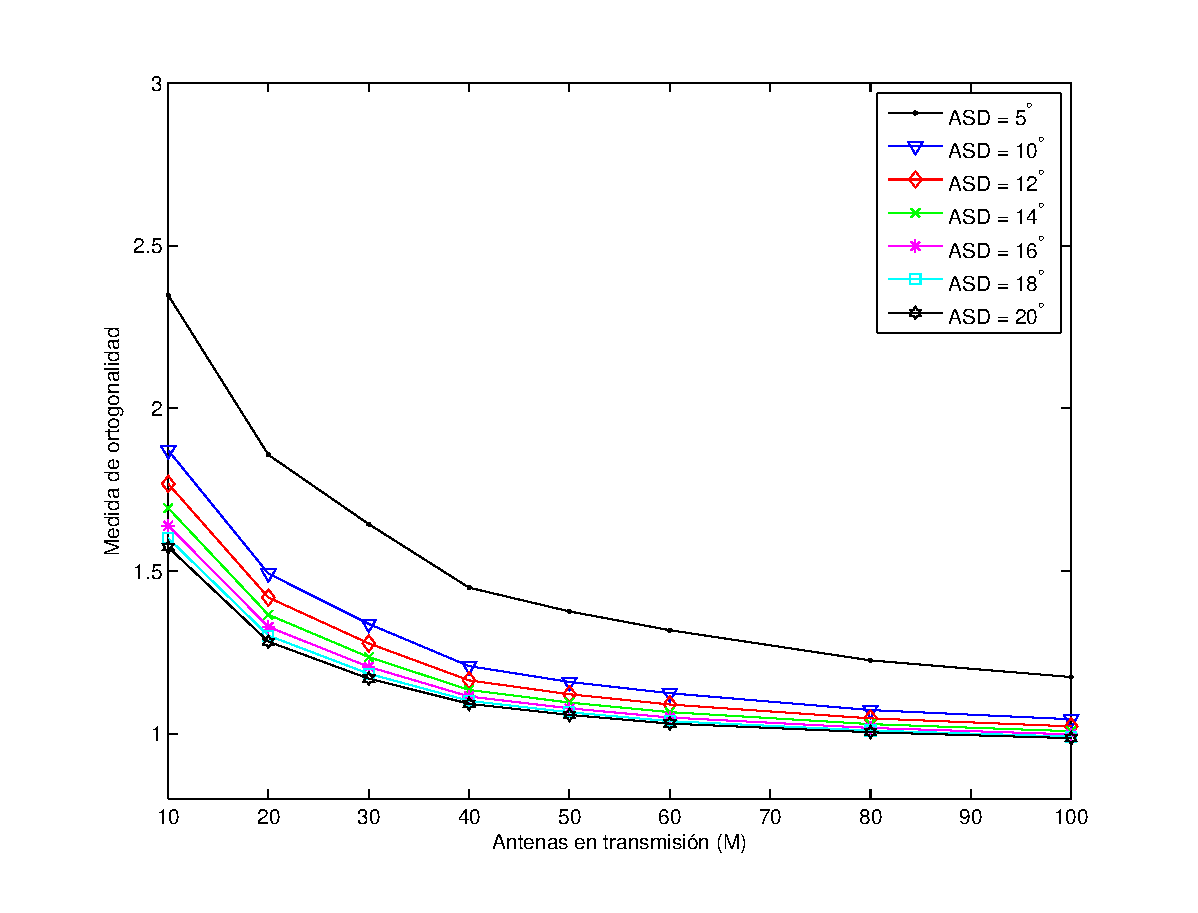
\includegraphics{figuras/orto_barridoM_N4dt1}}}}
	\caption{Medida de ortogonalidad para un sistema MIMO masivo con $M$ antenas transmisoras y $4$ antenas receptoras para diferentes valores de $ASD$ y $d_t$.}
	\label{fig:orto4}
\end{figure}




\subsection{Ortogonalidad en el caso sim�trico $N = M$}

Para el caso de sistemas MIMO sim�tricos, con igual n�mero de antenas receptoras que transmisoras ($M = N$), los resultados obtenidos son los que aparecen en la figura (\ref{fig:ortoN}). 

\begin{figure}[htbp]
\centering
	\mbox{ \subfigure[$ASD = 10^\circ$]{\resizebox{!}{10cm}		{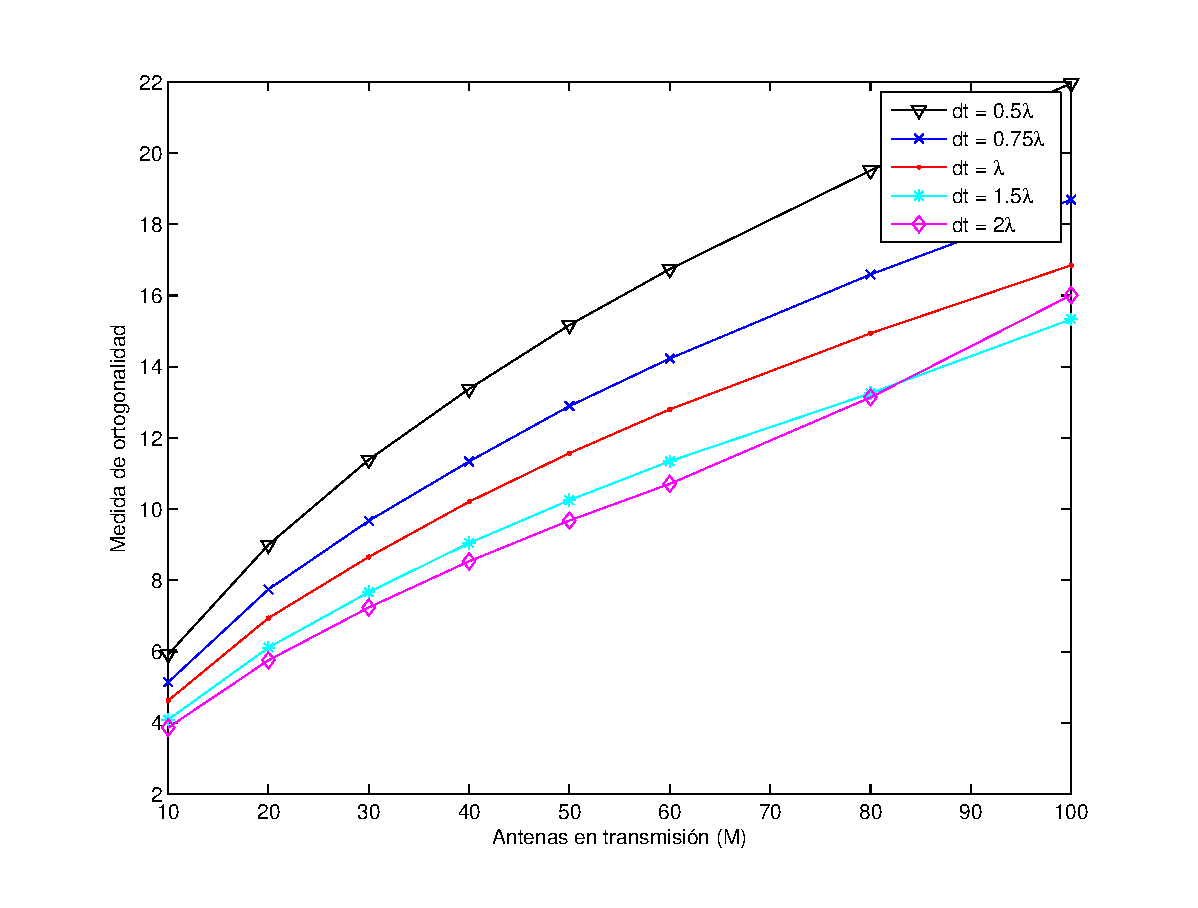
\includegraphics{figuras/orto_barridoM_NM_ASD10}}}}
	\mbox{ \subfigure[$d_t = \lambda$]{\resizebox{!}{10cm}		{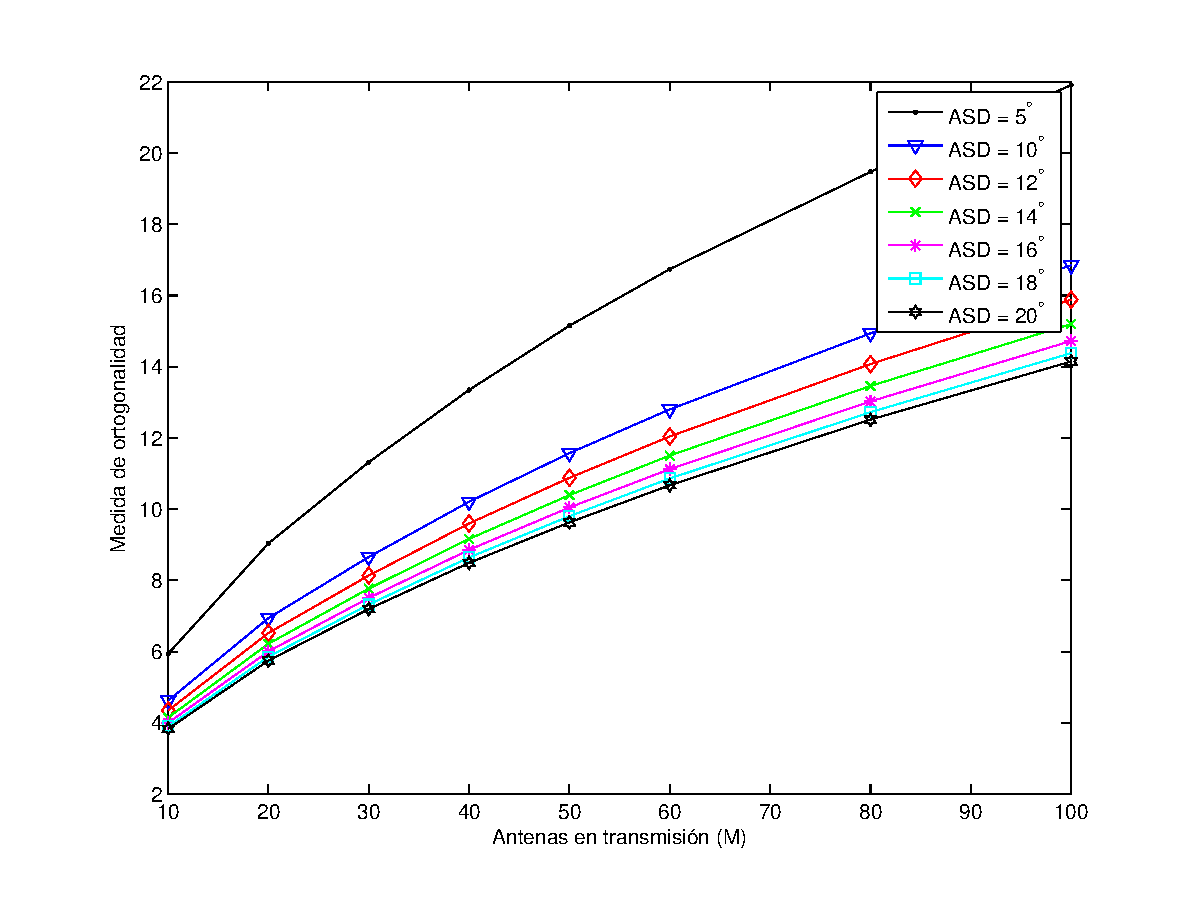
\includegraphics{figuras/orto_barridoM_NM_dt1}}}}
	\caption{Medida de ortogonalidad para un sistema MIMO  con igual n�mero de antenas transmisoras y receptoras para diferentes valores de $ASD$ y $d_t$.}
	\label{fig:ortoN}
\end{figure}


Podemos ver como los resultados en este caso son completamente diferentes que los obtenidos para los casos asim�tricos donde $N = 2$ y $N = 4$. Recordemos que estamos estudiando escenarios con sistemas MIMO masivo, donde el n�mero de antenas en un extremo de la comunicaci�n es significativamente mayor que el n�mero de antenas en el otro extremo, $M >> N$. En este caso, en el que $N = M$, no podemos aplicar las medidas que estamos estudiando pues no cumple el primer requisito que ha de tener un sistema MIMO masivo. Por ello, la conclusi�n que podemos extraer de este an�lisis es que no podremos lograr la ortogonalidad en matrices con dimensiones tan elevadas.

\subsection{Comparaci�n de ortogonalidad entre matrices realistas y matrices i.i.d.}

En esta �ltima secci�n compararemos la ortogonalidad entre las matrices que hemos generado de forma realista y las matrices i.i.d., con $M = 50$ antenas en el transmisor y diferente n�mero $N$ de antenas en el receptor. 

\begin{figure}[htbp]
\centering
	\mbox{ \subfigure[$ASD = 10^\circ$]{\resizebox{!}{10cm}		{\includegraphics{figuras/orto_M50_iid_ASD10}}}}
	\mbox{ \subfigure[$d_t = \lambda$]{\resizebox{!}{10cm}		{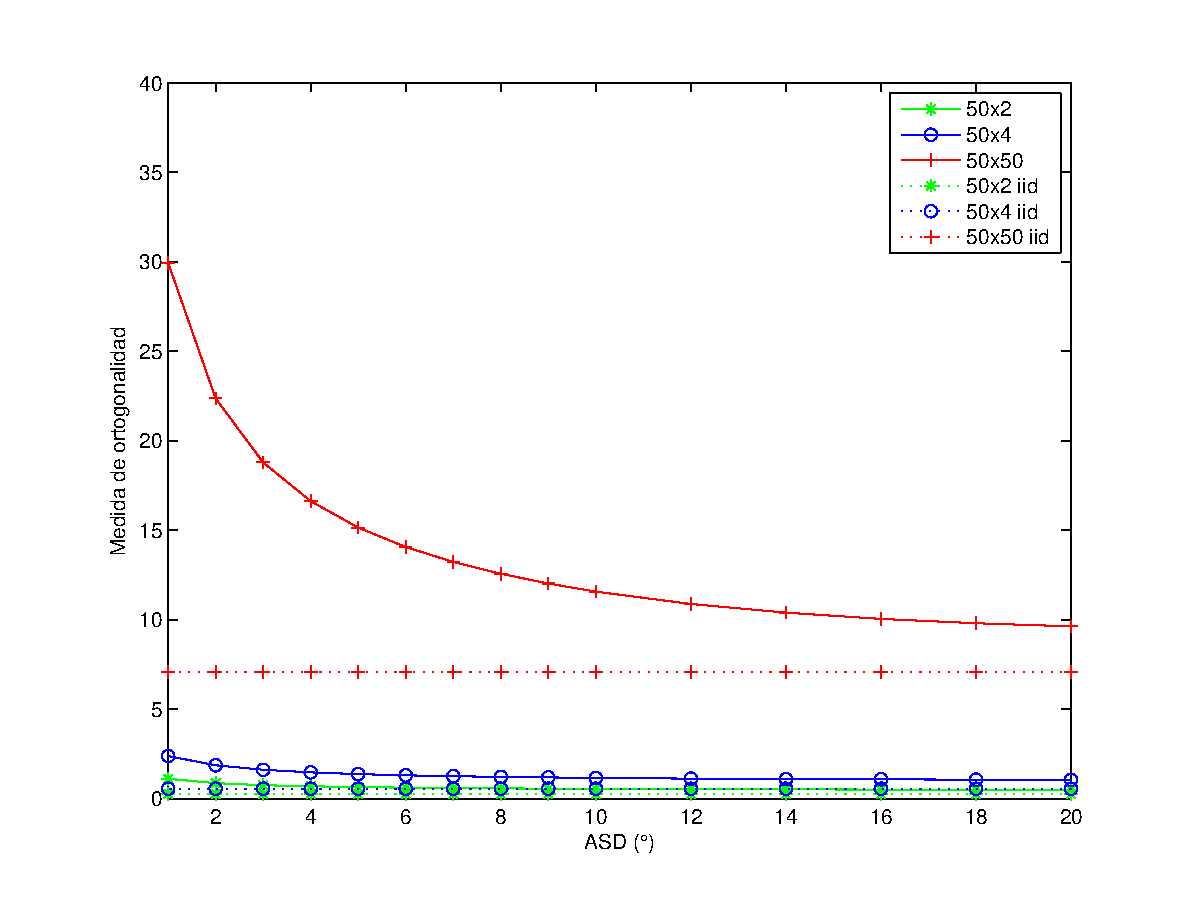
\includegraphics{figuras/orto_M50_iid_dt1}}}}
	\caption{Medida de ortogonalidad para un sistema MIMO  con $50$ antenas transmisoras y diferente n�mero de antenas receptoras para diferentes valores de $ASD$ y $d_t$.}
	\label{fig:ortoM50}
\end{figure}

Los par�metros de estas simulaciones han sido escogidos eligiendo un caso est�ndar en el transmisor: una distancia entre antenas de $d_t = \lambda$ y un �ngulo de dispersi�n de las antenas transmisoras de $ASD = 10^{\circ}$. Como vemos en la figura (\ref{fig:ortoM50}), en todo momento la ortogonalidad de las matrices reales tienden a acercarse a las i.i.d a medida que la distancia entre antenas o el �ngulo de dispersi�n aumenta, comportamiento que esper�bamos pues es cuando se da la menor interferencia entre antenas. Adem�s, la norma de las matrices realistas est� siempre por encima de las ideales y tiende a acercarse al valor ideal a medida que mejoramos las condiciones (aumentamos la $d_t$ o $ASD$, como ya vimos en las secciones anteriores). 






















%%%%%%%%%%%%%%%%%%%%%%%%%%%%%%%%%%%%%%%%%%%%%%%%%%


%%%%%%%%%%%%%%%%%%%%%%%%%%%%%%%%%%%%%%%%%%%%%%%%%%
%%                  CAPITULO 4                  %%
%%%%%%%%%%%%%%%%%%%%%%%%%%%%%%%%%%%%%%%%%%%%%%%%%%
\chapter{Conclusiones y l�neas futuras de trabajo}
\input{capitulo5/5_conclusiones.tex}
%%%%%%%%%%%%%%%%%%%%%%%%%%%%%%%%%%%%%%%%%%%%%%%%%%
%%%%%%%%%%%%%%%%%%%%%%%%%%%%%%%%%%%%%%%%%%%%%%%%%%%%%%%%%%%%%
%%%%%%%%%%%%%%%%%%%%%%%%%%%%%%%%%%%%%%%%%%%%%%%%%%%%%%%%%%%%%
%%%                      AP�NDICES                        %%%
%%%%%%%%%%%%%%%%%%%%%%%%%%%%%%%%%%%%%%%%%%%%%%%%%%%%%%%%%%%%%
%%%%%%%%%%%%%%%%%%%%%%%%%%%%%%%%%%%%%%%%%%%%%%%%%%%%%%%%%%%%%
\part[Anexos]{ANEXOS}
\appendix
%%%%%%%%%%%%%%%%%%%%%%%%%%%%%%%%%%%%%%%%%%%%%%%%%%%%%%%%%%%%%

%%%%%%%%%%%%%%%%%%%%%%%%%%%%%%%%%%%%%%%%%%%%%%%%%%
%%                  APENDICE 1                  %%
%%%%%%%%%%%%%%%%%%%%%%%%%%%%%%%%%%%%%%%%%%%%%%%%%%
%\appendix
%\clearpage
%\addappheadtoctoc
%\appendixpage
\chapter{Descomposici�n de matrices}

Se denomina \textit{autovalor} de la matriz cuadrada $\miA$ al valor escalar $\lambda$ para el cual existe un vector $\mix$ distinto de $\mathbf{0}$ tal que $\miA \mix = \lambda \mix$. Al vector $\mix$ se le llama \textit{autovector} de $\miA$ correspondiente a $\lambda$. Los autovalores de la matriz $\miA$ son aquellos que valores de $\lambda$ que satisfacen la \textit{ecuaci�n caracter�stica} de $\miA$, que se define como det[$\miA$ - $\lambda \mathbf{I}$] = 0. El polinomio en $\lambda$ definido por det[$\miA$ - $\lambda \mathbf{I}$] = 0 se llama \textit{polinomio caracter�stico} de $\miA$, por lo que los autovalores de $\miA$ son las ra�ces del polinomio caracter�stico. El polinomio caracter�stico de una matriz $N \times N$ tiene $N$ ra�ces �nicas $r_1, ..., r_N (r_i \neq r_j)$ si es de la forma  det[$\miA - \lambda \mathbf{I}$] = $(-1)^N(\lambda - r_1)...(\lambda - r_N)$. Cuando el polinomio caracter�stico incluye un t�rmino $(\lambda - r_i)^k, k>1$, decimos que la ra�z $r_i$ tiene multiplicidad $k$. Una matriz $N \times N$ tiene $N$ autovalores $\lambda_1, ... \lambda_N$, aunque no todos ellos tienen por qu� ser �nicos si alguna de las ra�ces tiene multiplicidad mayor que 1. Adem�s, el determinante de una matriz es el producto de todos los autovalores de la matriz
\footnote{
Esta propiedad es f�cilmente demostrable de la siguiente forma:
Suponiendo que $\lambda_1, ... \lambda_n$ son los autovalores de la matriz $\miA$. As�, como ya hemos dicho, los autovalores son tambi�n las ra�ces del polinomio caracter�stico
\begin{equation}
	det(\miA - \lambda \mathbf{I}) = p(\lambda) = (-1)^n(\lambda - \lambda_1)...(\lambda - \lambda_n) = (\lambda_1 - \lambda)...(\lambda_n - \lambda)
\end{equation}
As�, dando a $\lambda$ el valor 0, simplemente porque es una variable, 
\begin{equation}
	det(\miA) = \lambda_1 \lambda_2... \lambda_n
\end{equation}
es decir, el determinante de la matriz es igual al producto de sus autovalores}, 

teniendo en cuenta que un autovalor $r_i$ con multiplicidad $k$ contribuir� $r_i^k$ al producto. 

Los autovalores de una matriz herm�tica son siempre reales, aunque los autovectores pueden ser complejos. Adem�s, si $\miA$ es una matriz $N \times N$ se puede escribir como sigue:
\begin{equation}
	\miA = \mathbf{U} \mathbf{\Lambda} \mathbf{U}^H
\end{equation}
donde $\mathbf{U}$ es una matriz unitaria cuyas columnas son los autovectores de $\miA$ y $\mathbf{\Lambda}$ = diag[$\lambda_1$, ..., $\lambda_k$, 0, ..., 0]. Como ya hemos comentado, cuando $\miA$ es herm�tica, $\mathbf{\Lambda}$ tiene s�lo elementos reales. Decimos que la matriz  $\miA$ es \textit{definida positiva} si, para todos los vectores $\mix \neq 0$, tenemos que $\mix^H\miA\mix > 0$. Una matriz herm�tica es definida positiva si y s�lo si todos sus autovalores son positivos. De forma similar, la matriz $\miA$ es semidefinida positiva o definida no negativa si, para todos los vectores $\mix \neq 0$, $\miX^H\miA\mix \ge 0$. Una matriz herm�tica es definida no negativa si y s�lo si todos sus autovalores son no negativos. 

Suponiendo que la matriz $\miA$ es una matriz de dimensiones $N \times M$ y tiene rango $R_A$. Entonces existe una matriz $\mathbf{\Sigma}$ de dimensiones $N$x$M$, y dos matrices unitarias $\mathbf{U}$ y $\mathbf{V}$ cuadradas de tama�o $N \times M$ respectivamente tal que
\begin{equation}\label{svd}
\miA = \mathbf{U}\mathbf{\Sigma}\mathbf{V}^H
\end{equation}
Llamamos a las columnas de $\mathbf{V}$ los vectores singulares de $\miA$ por la derecha y las columnas de $\mathbf{U}$ los vectores singulares de $\miA$ por la izquierda. En cuanto a la matriz $\mathbf{\Sigma}$, es una matriz en cuya diagonal se encuentran los valores singulares de $\miA$ y todos los elementos fuera de la diagonal son cero

\begin{equation}
\mathbf{\Sigma}_{N \times M}=
\begin{bmatrix}
\sigma_1 & \cdots & 0\\
\vdots & \ddots & \vdots \\
0 & \cdots & \sigma_N
\end{bmatrix}\\ 
\end{equation}
para N = M. Para los casos en los que la matriz no es cuadrada:
\begin{equation}
\mathbf{\Sigma}_{N \times M}=
\begin{bmatrix}
\sigma_1 & \cdots & 0\\
\vdots & \ddots & \vdots \\
0 & \cdots & \sigma_N\\
0 & \cdots & 0\\
\vdots & \ddots & \vdots \\
0 & \cdots & 0\\
\end{bmatrix}\\ 
\end{equation}
para $N > M$, y
\begin{equation}
\mathbf{\Sigma}_{N \times M}=
\begin{bmatrix}
\sigma_1 & \cdots & 0 & 0 & \cdots & 0\\
\vdots & \ddots & \vdots  & \vdots &\ddots & \vdots\\
0 & \cdots & \sigma_N & 0 & \cdots & 0
\end{bmatrix}\\ 
\end{equation}
para $N < M$, donde $\sigma_i = \sqrt{\lambda_i}$ siendo $\sigma_i$ el valor singular $i$-�simo de la matriz $\miA\miA^H$ y $\lambda_i$ el autovalor $i$-�simo. A la descomposici�n descrita en (\ref{svd}) se le llama descomposici�n en valores singulares de $\miA$.







\label{anexo}
%%%%%%%%%%%%%%%%%%%%%%%%%%%%%%%%%%%%%%%%%%%%%%%%%%


\backmatter

%%%%%%%%%%%%%%%%%%%%%%%%%%%%%%%%%%%%%%%%%%%%%%%%%%
%%                 BIBLIOGRAF�A                 %%
%%%%%%%%%%%%%%%%%%%%%%%%%%%%%%%%%%%%%%%%%%%%%%%%%%
%
%\bibliographystyle{acm}
%%%% Para incluir bibliografia que no est� citada en el texto
%%% Hay que meter los libros que he ido usando. 
%\nocite{Goldsmith_book}
%\bibliography{bibliografia/bibliografia}

\bibliographystyle{unsrt}
\bibliography{bibliografia/bibliografia}


%\input{bibliografia/bibliografia}
%%%%%%%%%%%%%%%%%%%%%%%%%%%%%%%%%%%%%%%%%%%%%%%%%%

\end{document}
